\documentclass[11pt]{article}

\usepackage[a4paper,margin=1in]{geometry}
\usepackage{amsmath,amssymb,bm}
\usepackage{booktabs}
\usepackage{graphicx}
\usepackage{tikz}
\usetikzlibrary{arrows.meta, positioning, calc, decorations.pathreplacing}
\usepackage{hyperref}

\hypersetup{
    colorlinks=true,
    linkcolor=blue,
    citecolor=blue,
    urlcolor=blue
}

\title{An Analytical First-Order Mixed-Zonal Theory for GEqOE\\
\large Near-Identity Averaging with Direct Residue Decomposition}
\author{Jose Manuel Montilla García}
\date{\today}

\begin{document}
\maketitle

\begin{abstract}
This note presents a complete analytical first-order theory for the
Generalized Equinoctial Orbital Elements (GEqOE) under autonomous Earth zonal
harmonics through $J_5$, comprising closed-form mean-element equations,
closed-form short-period corrections, and closed-form osculating
reconstruction. For pure $J_2$ the mean propagation is itself closed-form;
for the general mixed-zonal model it reduces to a smooth, slowly varying ODE
that is orders of magnitude cheaper than osculating integration.
Three main results are established.
First, the GEqOE state vector admits an exact first-order orbit-averaging
operator in the generalized eccentric longitude $K$, yielding a finite
Fourier-harmonic mean-element system in the single slow angle
$\omega = \Psi - \Omega$. For pure $J_2$, the secular closure is especially
simple: $\nu$, $g$, and $Q$ are constant, while the equinoctial pairs
$(p_1,p_2)$ and $(q_1,q_2)$ undergo uniform rotations with explicit rates.
Second, a direct residue decomposition method is developed for constructing
the short-period kernels: by exploiting the fixed pole structure of the
$dM/dF$ Jacobian (where $F = e^{if}$ is the complex true anomaly exponential),
each kernel reduces to a polynomial-plus-simple-poles form that is free of
spurious logarithmic terms and scales gracefully to high zonal degree. The
resulting expressions are exact closed-form rational functions of $(q, Q)$,
precomputed once by symbolic algebra; at runtime the theory requires only the
evaluation of these algebraic formulas---no numerical quadrature, no
interpolation, no iterative solution (except the standard Kepler equation).
Third, the resulting analytical mean-plus-short-period model is validated
numerically against full osculating GEqOE Taylor integration, achieving
sub-kilometer osculating position reconstruction for low-eccentricity orbits
and few-kilometer reconstruction for high-eccentricity ($e = 0.65$) orbits
over 10+ orbital periods, with reconstruction errors scaling linearly with
the zonal perturbation parameter as expected for a first-order theory.
A controlled comparison against the Draper Semi-analytical Satellite Theory
(DSST, as implemented in Orekit) using the same zonal-only force model
reveals that the GEqOE theory outperforms DSST across all 12 test regimes
despite being two to three orders of magnitude faster per epoch. DSST
achieves better secular drift accuracy (due to its $J_2^2$ correction), but
this advantage is overwhelmed by the GEqOE theory's superior short-period
reconstruction: the closed-form rational expressions, exact in eccentricity,
produce 1.5--8$\times$ smaller osculating errors than DSST's
eccentricity-truncated Fourier series.
\end{abstract}

\section{Introduction}
\label{sec:intro}

This note develops the averaged formulation for the Generalized Equinoctial
Orbital Elements (GEqOE) of Ba\`u et al.~\cite{bau2021} under the autonomous
conservative case generated by the Earth zonal harmonics. The published GEqOE
set uses the generalized mean longitude $L$ as the fourth element; the present
work instead propagates the generalized eccentric longitude $K$, from which $L$
is recovered via the relation \eqref{eq:L_def}. The focus is on
the GEqOE state
\begin{equation}
\bm{y} = (\nu,p_1,p_2,K,q_1,q_2),
\end{equation}
under the following assumptions:
\begin{enumerate}
    \item the conservative perturbation is autonomous and axisymmetric about the
    inertial $z$ axis;
    \item the disturbing potential is a static zonal expansion truncated at
    degree $N$ (in practice $N = 5$);
    \item averaging is performed with respect to the propagated fast angle $K$;
    \item only first-order dynamics are derived: all quantities of order
    $O(J_n^2)$ and all cross-zonal products $O(J_n J_m)$ are neglected.
\end{enumerate}

The first-order near-identity averaging approach follows the Lie-transform
perturbation tradition of Deprit~\cite{deprit1969} and
Hori~\cite{hori1966}, adapted to the non-canonical GEqOE variables.
The restriction to autonomous axisymmetric perturbations is deliberate. It
keeps the averaged problem autonomous and avoids the additional complications
introduced by explicit time dependence (third-body ephemerides,
rotating-frame geopotential tides, etc.).

The classical analytical treatment of the zonal satellite problem originates
with Brouwer~\cite{brouwer1959} and Kozai~\cite{kozai1959}, who derived
first-order periodic and second-order secular corrections in canonical
variables. Subsequent developments by Coffey and Deprit~\cite{coffey1982}
extended the theory to third order, while
de~Saedeleer~\cite{desaedeleer2005} provided a generic compact first-order
closed-form solution for any individual zonal harmonic.
Lara~\cite{lara2021} recently revisited the complete Brouwer solution using
a single canonical transformation in Poincar\'e style. In parallel,
non-singular equinoctial elements~\cite{broucke1972,cefola1972} provided the
foundation for the Draper Semi-analytical Satellite Theory (DSST), which
formulates the mean-element equations in equinoctial variables and in some
implementations evaluates the short-period corrections by numerical
quadrature~\cite{sanjuan2022}. The present work differs from these in that
it operates directly in the GEqOE variables of~\cite{bau2021}---which are
non-canonical and free of the circular-orbit and equatorial singularities
(though still singular for retrograde equatorial and rectilinear
orbits)---and replaces the Hamiltonian Lie series machinery with a direct
residue decomposition in the complex true anomaly variable~$F$.

The note is organized as follows.
Sections~\ref{sec:prelim}--\ref{sec:j2} establish the GEqOE dynamics, the
averaging operator, and the especially simple $J_2$ secular closure.
Section~\ref{sec:near_identity} develops the near-identity transformation
theory and the constructive first-order short-period map.
Sections~\ref{sec:complex_tav}--\ref{sec:residue} introduce the complex
true anomaly variables and the direct residue decomposition algorithm that
makes the short-period kernels tractable through high zonal degree.
Section~\ref{sec:operational} summarizes the operational structure of the
resulting analytical theory and clarifies the role of mean-state propagation.
Section~\ref{sec:general_zonal} analyzes the finite-harmonic structure of
the general zonal mean drift.
Section~\ref{sec:validation} validates the complete model against osculating
GEqOE Taylor integration.
Section~\ref{sec:thrust} sketches the path to a Fourier-in-$K$ thrust
extension, and Section~\ref{sec:conclusions} summarizes the conclusions.

\section{GEqOE Preliminaries}
\label{sec:prelim}

Define the auxiliary quantities
\begin{align}
g^2 &= p_1^2 + p_2^2, \qquad \beta = \sqrt{1-g^2}, \qquad
\alpha = \frac{1}{1+\beta}, \\
a &= \left(\frac{\mu}{\nu^2}\right)^{1/3}, \\
Q^2 &= q_1^2 + q_2^2, \qquad
\gamma = 1 + Q^2, \qquad
\delta = 1 - Q^2.
\end{align}
From the equinoctial orientation variables one has
\begin{equation}
\cos i = \frac{\delta}{\gamma},
\qquad
\tan\frac{i}{2} = Q.
\end{equation}

The propagated generalized eccentric longitude $K$ gives
\begin{align}
r &= a\left(1 - p_1 \sin K - p_2 \cos K\right), \label{eq:rK}\\
X &= a\left(\alpha p_1 p_2 \sin K + (1-\alpha p_1^2)\cos K - p_2\right), \\
Y &= a\left(\alpha p_1 p_2 \cos K + (1-\alpha p_2^2)\sin K - p_1\right),
\end{align}
and the normalized inertial $z$ coordinate is
\begin{equation}
\hat z = \frac{2(Yq_2 - Xq_1)}{\gamma r}. \label{eq:zhat}
\end{equation}

The generalized angular momentum used throughout~\cite{bau2021} and the
current implementation is
\begin{equation}
c = \left(\frac{\mu^2}{\nu}\right)^{1/3}\beta. \label{eq:cdef}
\end{equation}
Under purely conservative autonomous dynamics, the generalized energy is a first
integral and therefore
\begin{equation}
\dot{\nu} = 0.
\end{equation}

\section{Autonomous Zonal GEqOE Dynamics}

For a zonal potential of the form
\begin{equation}
U(r,\hat z) = \sum_{n\ge 2} U_n(r,\hat z)
= \sum_{n\ge 2} \frac{C_n}{r^{n+1}} P_n(\hat z),
\qquad
C_n = \mu J_n R_e^n,
\end{equation}
the current branch uses the exact conservative GEqOE system
\begin{align}
\dot{\nu} &= 0, \\
\dot{p}_1 &= p_2(d-w_h)
+ \frac{1}{c}\left(\frac{X}{a}+2p_2\right)\mathcal{E}_Z, \label{eq:p1_zonal}\\
\dot{p}_2 &= p_1(w_h-d)
- \frac{1}{c}\left(\frac{Y}{a}+2p_1\right)\mathcal{E}_Z, \label{eq:p2_zonal}\\
\dot{K} &= \frac{w}{r} + d - w_h
+ \frac{1}{c}\left(1+\alpha\left(1-\frac{r}{a}\right)\right)\mathcal{E}_Z, \\
\dot{q}_1 &= \frac{\gamma}{2} w_Y, \label{eq:q1_zonal}\\
\dot{q}_2 &= \frac{\gamma}{2} w_X, \label{eq:q2_zonal}
\end{align}
with
\begin{align}
w &= \sqrt{\frac{\mu}{a}}, \\
h &= \sqrt{c^2 - 2r^2 U}, \\
d &= \frac{h-c}{r^2}, \\
\mathcal{E}_Z &= \sum_{n\ge 2} (1-n) U_n, \\
F_h &= - \frac{\delta}{\gamma r}\,\frac{\partial U}{\partial \hat z}, \\
w_X &= \frac{X}{h}F_h, \qquad
w_Y = \frac{Y}{h}F_h, \qquad
w_h = w_X q_1 - w_Y q_2.
\end{align}

This formulation is already structurally suitable for averaging because:
\begin{enumerate}
    \item the system is autonomous;
    \item the fast angle is explicit;
    \item $\dot{\nu}=0$ exactly;
    \item all forcing enters through $r(K)$, $X(K)$, $Y(K)$, and $\hat z(K)$.
\end{enumerate}

\section{First-Order Orbit Averaging in \texorpdfstring{$K$}{K}}
\label{sec:avg}

\subsection{Averaging operator}

To first order in the zonal perturbation, the unperturbed fast flow is
\begin{equation}
\dot{K}_0 = \frac{w}{r},
\qquad
\frac{dt}{dK} = \frac{r}{w}.
\end{equation}
Hence the orbital average of any $2\pi$-periodic quantity $f(K)$ is
\begin{equation}
\langle f \rangle_K
= \frac{1}{T}\int_0^T f\,dt
= \frac{1}{2\pi a}\int_0^{2\pi} r(K)\,f(K)\,dK.
\label{eq:avg_operator}
\end{equation}

Let the slow state be
\begin{equation}
\bm{z} = (\nu,p_1,p_2,q_1,q_2).
\end{equation}
Then the exact first-order averaged slow flow of the autonomous zonal problem is
\begin{align}
\dot{\bar\nu} &= 0, \\
\dot{\bar p}_1 &=
\frac{1}{2\pi \bar a}\int_0^{2\pi} \bar r
\left[
\bar p_2(\bar d-\bar w_h)
+ \frac{1}{\bar c}\left(\frac{\bar X}{\bar a}+2\bar p_2\right)\bar{\mathcal E}_Z
\right]\,dK, \label{eq:avg_p1_general}\\
\dot{\bar p}_2 &=
\frac{1}{2\pi \bar a}\int_0^{2\pi} \bar r
\left[
\bar p_1(\bar w_h-\bar d)
- \frac{1}{\bar c}\left(\frac{\bar Y}{\bar a}+2\bar p_1\right)\bar{\mathcal E}_Z
\right]\,dK, \label{eq:avg_p2_general}\\
\dot{\bar q}_1 &=
\frac{1}{2\pi \bar a}\int_0^{2\pi}
\bar r \,\frac{\bar\gamma}{2}\,\bar w_Y\,dK, \label{eq:avg_q1_general}\\
\dot{\bar q}_2 &=
\frac{1}{2\pi \bar a}\int_0^{2\pi}
\bar r \,\frac{\bar\gamma}{2}\,\bar w_X\,dK. \label{eq:avg_q2_general}
\end{align}
All barred intermediate quantities are evaluated from the frozen slow state
$\bar{\bm z}$ and the fast phase $K$ via the unperturbed relations
\eqref{eq:rK}-\eqref{eq:zhat} and \eqref{eq:cdef}.

\subsection{Interpretation}

Equations \eqref{eq:avg_p1_general}-\eqref{eq:avg_q2_general} are already a
valid first-order mean-element model for any autonomous zonal expansion.
They are not yet a closed analytical solution, but they are an exact
one-revolution quadrature formula in the variables used by the present branch.

This is the right point of departure because it separates the
problem into two layers:
\begin{enumerate}
    \item a \emph{formal averaging layer}, which is already solved by
    \eqref{eq:avg_operator}-\eqref{eq:avg_q2_general};
    \item a \emph{closure layer}, where one asks whether the integrals can be
    reduced to explicit analytical expressions.
\end{enumerate}

\section{Closed First-Order \texorpdfstring{$J_2$}{J2} Secular Model}
\label{sec:j2}

\subsection{Why \texorpdfstring{$J_2$}{J2} is special}

For the pure $J_2$ potential,
\begin{equation}
U_{J_2} = -\frac{A}{r^3}\left(1-3\hat z^2\right),
\qquad
A = \frac{\mu J_2 R_e^2}{2},
\end{equation}
the averaged disturbing function is exceptionally simple. Using the standard
Keplerian averages
\begin{equation}
\left\langle \frac{1}{r^3}\right\rangle
= \frac{1}{a^3\beta^3},
\qquad
\left\langle \frac{\sin^2 u}{r^3}\right\rangle
= \frac{1}{2a^3\beta^3},
\end{equation}
with $u=\omega+f$, one obtains
\begin{equation}
\bar U_{J_2}
= -\frac{A}{2a^3\beta^3}\left(3\cos^2 i - 1\right)
= -\frac{A}{2a^3\beta^3}
\left(3\frac{\delta^2}{\gamma^2} - 1\right).
\label{eq:Ubar_J2}
\end{equation}

Equation \eqref{eq:Ubar_J2} depends only on $a$, $\beta$, and $i$. It has no
dependence on the node or pericenter angles. Consequently, at first order in
$J_2$,
\begin{equation}
\dot{\bar\nu} = 0,
\qquad
\dot{\bar g} = 0,
\qquad
\dot{\bar Q} = 0.
\end{equation}
Thus the magnitudes of $(p_1,p_2)$ and $(q_1,q_2)$ are constant and the secular
dynamics reduce to pure rotations.

\subsection{Secular rates}

Let
\begin{equation}
c_i = \cos i = \frac{\delta}{\gamma},
\qquad
p = a\beta^2.
\end{equation}
Within first-order singly averaged $J_2$ theory, the secular drift of the mean
GEqOE angular variables coincides with the classical $J_2$ secular
drift~\cite{brouwer1959,kozai1959} written in the GEqOE angles $\Psi$ and
$\Omega$.
At first order in $J_2$, the secular nodal rate is
\begin{equation}
\omega_{\Omega,J_2}
= -\frac{3}{2}\,\nu J_2
\left(\frac{R_e}{p}\right)^2 c_i
= -\frac{3A}{c a^3 \beta^3}\,\frac{\delta}{\gamma},
\label{eq:OmegaJ2}
\end{equation}
and the secular rate of the generalized longitude of pericenter is
\begin{equation}
\omega_{\Psi,J_2}
= \frac{3}{4}\,\nu J_2
\left(\frac{R_e}{p}\right)^2
\left(5c_i^2 - 2c_i - 1\right)
= \frac{3A}{2c a^3 \beta^3}
\left(
5\frac{\delta^2}{\gamma^2}
- 2\frac{\delta}{\gamma}
- 1
\right).
\label{eq:PsiJ2}
\end{equation}

Because
\begin{equation}
p_1 = g\sin\Psi,
\qquad
p_2 = g\cos\Psi,
\qquad
q_1 = Q\sin\Omega,
\qquad
q_2 = Q\cos\Omega,
\end{equation}
the first-order mean GEqOE system for $J_2$ becomes
\begin{align}
\dot{\bar\nu} &= 0, \label{eq:j2_mean_nu}\\
\dot{\bar p}_1 &= \omega_{\Psi,J_2}\,\bar p_2, \label{eq:j2_mean_p1}\\
\dot{\bar p}_2 &= -\omega_{\Psi,J_2}\,\bar p_1, \label{eq:j2_mean_p2}\\
\dot{\bar q}_1 &= \omega_{\Omega,J_2}\,\bar q_2, \label{eq:j2_mean_q1}\\
\dot{\bar q}_2 &= -\omega_{\Omega,J_2}\,\bar q_1. \label{eq:j2_mean_q2}
\end{align}

Equations \eqref{eq:j2_mean_nu}-\eqref{eq:j2_mean_q2} are autonomous and closed.
They provide exactly the kind of reduced slow-flow model that is suitable for
fast metric computation.

\subsection{Closed-form integration}

Because the coefficients in
\eqref{eq:j2_mean_p1}-\eqref{eq:j2_mean_q2} are constant along the secular
$J_2$ flow, the system is explicitly integrable. Define the mean angular
variables
\begin{equation}
\bar\Psi = \operatorname{atan2}(\bar p_1,\bar p_2),
\qquad
\bar\Omega = \operatorname{atan2}(\bar q_1,\bar q_2).
\end{equation}
Then
\begin{equation}
\dot{\bar\Psi} = \omega_{\Psi,J_2},
\qquad
\dot{\bar\Omega} = \omega_{\Omega,J_2},
\end{equation}
so that
\begin{equation}
\bar\Psi(t) = \bar\Psi_0 + \omega_{\Psi,J_2}(t-t_0),
\qquad
\bar\Omega(t) = \bar\Omega_0 + \omega_{\Omega,J_2}(t-t_0).
\end{equation}

Let
\begin{equation}
\bar g_0 = \sqrt{\bar p_1(t_0)^2 + \bar p_2(t_0)^2},
\qquad
\bar Q_0 = \sqrt{\bar q_1(t_0)^2 + \bar q_2(t_0)^2}.
\end{equation}
The closed secular solution is therefore
\begin{align}
\bar\nu(t) &= \bar\nu_0, \\
\bar p_1(t) &= \bar g_0
\sin\!\left[\bar\Psi_0 + \omega_{\Psi,J_2}(t-t_0)\right], \\
\bar p_2(t) &= \bar g_0
\cos\!\left[\bar\Psi_0 + \omega_{\Psi,J_2}(t-t_0)\right], \\
\bar q_1(t) &= \bar Q_0
\sin\!\left[\bar\Omega_0 + \omega_{\Omega,J_2}(t-t_0)\right], \\
\bar q_2(t) &= \bar Q_0
\cos\!\left[\bar\Omega_0 + \omega_{\Omega,J_2}(t-t_0)\right].
\label{eq:j2_closed_form}
\end{align}

Equivalently, the two equinoctial pairs evolve by constant-speed planar
rotations,
\begin{equation}
\begin{bmatrix}
\bar p_1(t) \\
\bar p_2(t)
\end{bmatrix}
=
\begin{bmatrix}
\cos\theta_\Psi & \sin\theta_\Psi \\
-\sin\theta_\Psi & \cos\theta_\Psi
\end{bmatrix}
\begin{bmatrix}
\bar p_1(t_0) \\
\bar p_2(t_0)
\end{bmatrix},
\qquad
\theta_\Psi = \omega_{\Psi,J_2}(t-t_0),
\end{equation}
\begin{equation}
\begin{bmatrix}
\bar q_1(t) \\
\bar q_2(t)
\end{bmatrix}
=
\begin{bmatrix}
\cos\theta_\Omega & \sin\theta_\Omega \\
-\sin\theta_\Omega & \cos\theta_\Omega
\end{bmatrix}
\begin{bmatrix}
\bar q_1(t_0) \\
\bar q_2(t_0)
\end{bmatrix},
\qquad
\theta_\Omega = \omega_{\Omega,J_2}(t-t_0).
\end{equation}

\subsection{Mean longitude / phase}

If a mean fast phase is also required, the natural choice is the mean
generalized longitude
\begin{equation}
\bar L = \bar M + \bar\Psi.
\end{equation}
Using the standard first-order $J_2$ secular rate of the mean anomaly,
\begin{equation}
\dot{\bar M}
= \nu
+ \frac{3}{4}\,\nu J_2
\left(\frac{R_e}{a\beta^2}\right)^2
\beta\left(3c_i^2-1\right),
\end{equation}
one obtains
\begin{equation}
\dot{\bar L}
= \nu
+ \frac{3}{4}\,\nu J_2
\left(\frac{R_e}{a\beta^2}\right)^2
\left[
\beta(3c_i^2-1)
+ 5c_i^2 - 2c_i - 1
\right].
\label{eq:Lbar_J2}
\end{equation}

\section{Near-Identity Transformation and Short-Period Map}
\label{sec:near_identity}

\subsection{Near-identity transformation}

A complete mean-element formulation requires more than the secular equations.
It also requires a \emph{near-identity
transformation}~\cite{deprit1969,hori1966} between:
\begin{enumerate}
    \item the osculating GEqOE of the full zonal dynamics, and
    \item the mean GEqOE propagated by the secular model.
\end{enumerate}

Write the exact first-order zonal problem in the form
\begin{align}
\dot{\bm z} &= \varepsilon \bm f_1(\bm z,K) + O(\varepsilon^2), \\
\dot K &= n_0(\bm z,K) + \varepsilon g_1(\bm z,K) + O(\varepsilon^2),
\label{eq:j2_fast_slow_form}
\end{align}
where
\begin{equation}
\bm z = (\nu,p_1,p_2,q_1,q_2),
\qquad
\varepsilon \sim J_n,
\qquad
n_0(\bm z,K) = \frac{w}{r}.
\end{equation}

The complete averaged formulation is then sought in the form
\begin{align}
\bm z_{\mathrm{osc}}
&= \bar{\bm z}
+ \varepsilon \bm u_1(\bar{\bm z},\bar K)
+ O(\varepsilon^2), \label{eq:forward_map_z}\\
K_{\mathrm{osc}}
&= \bar K
+ \varepsilon v_1(\bar{\bm z},\bar K)
+ O(\varepsilon^2), \label{eq:forward_map_K}
\end{align}
with periodic short-period corrections $\bm u_1$ and $v_1$.

The usual normalization is
\begin{equation}
\frac{1}{2\pi}\int_0^{2\pi} \bm u_1(\bar{\bm z},\bar K)\,d\bar K = \bm 0,
\qquad
\frac{1}{2\pi}\int_0^{2\pi} v_1(\bar{\bm z},\bar K)\,d\bar K = 0,
\label{eq:zero_mean_norm}
\end{equation}
which fixes the decomposition into mean and periodic parts.

The inverse initialization map, used to convert osculating initial conditions
to mean initial conditions, follows directly from
\eqref{eq:forward_map_z}-\eqref{eq:forward_map_K}:
\begin{align}
\bar{\bm z}(t_0)
&= \bm z_{\mathrm{osc}}(t_0)
- \varepsilon \bm u_1\!\left(\bm z_{\mathrm{osc}}(t_0),K_{\mathrm{osc}}(t_0)\right)
+ O(\varepsilon^2), \label{eq:inverse_map_z}\\
\bar K(t_0)
&= K_{\mathrm{osc}}(t_0)
- \varepsilon v_1\!\left(\bm z_{\mathrm{osc}}(t_0),K_{\mathrm{osc}}(t_0)\right)
+ O(\varepsilon^2).
\label{eq:inverse_map_K}
\end{align}
The $O(\varepsilon^2)$ initialization error incurred by evaluating $\bm u_1$
at the osculating state instead of the (unknown) mean state is consistent
with the first-order theory.

\subsection{Homological equations}

Substituting \eqref{eq:forward_map_z}-\eqref{eq:forward_map_K} into
\eqref{eq:j2_fast_slow_form} and matching terms at first order gives the
homological equation for the slow variables:
\begin{equation}
n_0(\bar{\bm z},\bar K)
\frac{\partial \bm u_1}{\partial \bar K}
= \bm f_1(\bar{\bm z},\bar K)
- \bar{\bm f}_1(\bar{\bm z}),
\label{eq:homological_u}
\end{equation}
where $\bar{\bm f}_1$ is the averaged slow drift. Therefore
\begin{equation}
\frac{\partial \bm u_1}{\partial \bar K}
= \frac{\bar r}{\bar w}
\left[
\bm f_1(\bar{\bm z},\bar K)
- \bar{\bm f}_1(\bar{\bm z})
\right].
\label{eq:u_prime}
\end{equation}
Once the secular drift is known, the short-period correction of the slow
variables is obtained by a direct quadrature in $\bar K$:
\begin{equation}
\bm u_1(\bar{\bm z},\bar K)
= \int^{\bar K}
\frac{\bar r(\phi)}{\bar w}
\left[
\bm f_1(\bar{\bm z},\phi)
- \bar{\bm f}_1(\bar{\bm z})
\right] d\phi
- \text{(constant chosen to enforce \eqref{eq:zero_mean_norm})}.
\label{eq:u_integral}
\end{equation}

The phase correction is slightly more delicate because the unperturbed fast rate
$n_0=w/r$ depends on $\bar K$. The first-order phase homological equation is
\begin{equation}
n_0\frac{\partial v_1}{\partial \bar K}
- \frac{\partial n_0}{\partial \bar K}v_1
= g_1 - \bar g_1
+ \frac{\partial n_0}{\partial \bar{\bm z}}\cdot \bm u_1,
\label{eq:homological_v}
\end{equation}
which can be rewritten as
\begin{equation}
\frac{\partial}{\partial \bar K}
\left(
\frac{v_1}{n_0}
\right)
= \frac{
g_1 - \bar g_1
+ \dfrac{\partial n_0}{\partial \bar{\bm z}}\cdot \bm u_1
}{
n_0^2
}.
\label{eq:v_prime}
\end{equation}
Hence $v_1$ is also obtained by quadrature, again with the additive constant
fixed by the zero-mean normalization in \eqref{eq:zero_mean_norm}.

\subsection{Constructive first-order map in anomaly variables}

The previous discussion becomes constructive once the zonal forcing is written
in variables adapted to the unperturbed ellipse. Introduce
\begin{equation}
G = K - \Psi,
\qquad
\omega = \Psi - \Omega,
\qquad
s_i = \sin i = \frac{2Q}{\gamma},
\qquad
c_i = \cos i = \frac{\delta}{\gamma}.
\end{equation}
Then the unperturbed geometry is
\begin{align}
r &= a(1-g\cos G), \\
\cos f &= \frac{\cos G - g}{1-g\cos G}, \\
\sin f &= \frac{\beta \sin G}{1-g\cos G}, \\
u &= \omega + f,
\end{align}
and therefore
\begin{equation}
\hat z = s_i \sin u.
\end{equation}

To first order in $J_2$ one may set
\begin{equation}
h = c + O(J_2),
\qquad
d = -\frac{U}{c} + O(J_2^2),
\qquad
w_h = \frac{3A}{c r^3} c_i \hat z^2 + O(J_2^2),
\end{equation}
with
\begin{equation}
U = -\frac{A}{r^3}\left(1-3s_i^2\sin^2 u\right).
\end{equation}

Now parameterize the slow variables by $(\nu,g,\Psi,Q,\Omega)$ rather than by
$(\nu,p_1,p_2,q_1,q_2)$. Using
\begin{equation}
p_1 = g\sin\Psi,
\quad
p_2 = g\cos\Psi,
\quad
q_1 = Q\sin\Omega,
\quad
q_2 = Q\cos\Omega,
\end{equation}
and the exact GEqOE zonal equations, the first-order osculating dynamics become
\begin{align}
\dot \nu &= 0, \\
\dot g &=
\frac{U}{c}\,\beta \sin G
= -\frac{A\beta}{c r^3}
\left(1-3s_i^2\sin^2 u\right)\sin G,
\label{eq:gdot_j2_first}\\
\dot Q &=
-\frac{6A Q c_i}{c r^3}\sin u \cos u,
\label{eq:Qdot_j2_first}\\
\dot\Omega &=
-\frac{6A c_i}{c r^3}\sin^2 u,
\label{eq:Omegadot_j2_first}\\
\dot\Psi &=
d - w_h - \frac{U}{c}\left(1 + \frac{\cos G}{g}\right)
+ O(J_2^2).
\label{eq:Psidot_j2_first}
\end{align}

Equations \eqref{eq:gdot_j2_first}-\eqref{eq:Psidot_j2_first} show the
main structural point: once expressed through $(G,u)$, the first-order forcing
is a trigonometric-rational function of the anomaly.

The $\dot\Psi$ expression must be derived directly from the exact GEqOE
$p_1,p_2$ equations,
\begin{equation}
\dot\Psi = \frac{p_2 \dot p_1 - p_1 \dot p_2}{g^2},
\end{equation}
not by shortcut analogy. For the zonal GEqOE right-hand side this gives
\begin{equation}
\dot\Psi = d - w_h + \frac{\mathcal E_Z}{c}
\left(1 + \frac{\cos G}{g}\right),
\end{equation}
and therefore \eqref{eq:Psidot_j2_first} for $J_2$ with
$\mathcal E_Z = -U$.

Multiplying by
\begin{equation}
\frac{dt}{dG} = \frac{r}{w} + O(J_2)
\end{equation}
gives the anomaly-form equations for the short-period map. For the two
magnitude variables:
\begin{align}
\frac{dg}{dG}
&= -\frac{A}{\mu r^2}
\left(1-3s_i^2\sin^2 u\right)\sin G,
\label{eq:dg_dG}\\
\frac{dQ}{dG}
&= -\frac{6A Q c_i}{\mu \beta r^2}\sin u \cos u.
\label{eq:dQ_dG}
\end{align}
For the two angles:
\begin{align}
\frac{d\Omega}{dG}
&= -\frac{6A c_i}{\mu \beta r^2}\sin^2 u,
\label{eq:dOmega_dG}\\
\frac{d\Psi}{dG}
&= \frac{r}{w}\,\dot\Psi
 = \frac{r}{w}
\left[
d - w_h - \frac{U}{c}\left(1 + \frac{\cos G}{g}\right)
\right].
\label{eq:dPsi_dG}
\end{align}

The mean-to-osculating short-period corrections are now obtained by subtracting
the secular pieces and integrating over $G$:
\begin{align}
\mathcal G_1'(G) &=
\frac{dg}{dG}, \qquad
\langle \mathcal G_1 \rangle = 0, \\
\mathcal Q_1'(G) &=
\frac{dQ}{dG}, \qquad
\langle \mathcal Q_1 \rangle = 0, \\
\mathcal N_1'(G) &=
\frac{d\Omega}{dG}
- \frac{r}{w}\,\omega_{\Omega,J_2},
\qquad
\langle \mathcal N_1 \rangle = 0, \\
\mathcal P_1'(G) &=
\frac{d\Psi}{dG}
- \frac{r}{w}\,\omega_{\Psi,J_2},
\qquad
\langle \mathcal P_1 \rangle = 0.
\label{eq:map_primes}
\end{align}

Hence the first-order map can be written as
\begin{align}
g_{\mathrm{osc}} &= \bar g + \mathcal G_1(\bar G) + O(J_2^2), \\
Q_{\mathrm{osc}} &= \bar Q + \mathcal Q_1(\bar G) + O(J_2^2), \\
\Psi_{\mathrm{osc}} &= \bar\Psi + \mathcal P_1(\bar G) + O(J_2^2), \\
\Omega_{\mathrm{osc}} &= \bar\Omega + \mathcal N_1(\bar G) + O(J_2^2),
\label{eq:explicit_map_gQPsiOmega}
\end{align}
where $\bar G = \bar K - \bar\Psi$.

Finally, the GEqOE components follow immediately:
\begin{align}
p_{1,\mathrm{osc}} &= g_{\mathrm{osc}}\sin\Psi_{\mathrm{osc}}, \\
p_{2,\mathrm{osc}} &= g_{\mathrm{osc}}\cos\Psi_{\mathrm{osc}}, \\
q_{1,\mathrm{osc}} &= Q_{\mathrm{osc}}\sin\Omega_{\mathrm{osc}}, \\
q_{2,\mathrm{osc}} &= Q_{\mathrm{osc}}\cos\Omega_{\mathrm{osc}}.
\label{eq:pq_from_map}
\end{align}

\subsection{First-order fast-phase map in \texorpdfstring{$L$}{L} and \texorpdfstring{$K$}{K}}

The missing fast-phase piece can be written just as explicitly. Introduce the
generalized longitude
\begin{equation}
L = K + p_1 \cos K - p_2 \sin K,
\label{eq:L_def}
\end{equation}
so that, for the unperturbed geometry,
\begin{equation}
\frac{\partial L}{\partial K}
= 1 - p_1 \sin K - p_2 \cos K
= \frac{r}{a}.
\label{eq:dLdK}
\end{equation}

At first order in $J_2$ the forward longitude map is
\begin{equation}
L_{\mathrm{osc}}
= \bar L + \ell_1(\bar{\bm z},\bar K) + O(J_2^2),
\label{eq:forward_map_L}
\end{equation}
with $\ell_1$ normalized by
\begin{equation}
\frac{1}{2\pi}\int_0^{2\pi}\ell_1(\bar{\bm z},\bar K)\,d\bar K = 0.
\label{eq:ell_zero_mean}
\end{equation}
For the conservative zonal problem, the exact GEqOE $L$ equation reduces at
first order to
\begin{equation}
\dot L
= \nu + d - w_h
- \frac{U}{c}\left[
\frac{1}{\alpha} + \alpha\left(1-\frac{r}{a}\right)
\right]
+ O(J_2^2),
\label{eq:Ldot_j2_first}
\end{equation}
and therefore
\begin{equation}
\ell_1'(\bar K)
= \frac{\bar r}{\bar w}
\left[
\dot L(\bar{\bm z},\bar K)
- \langle \dot L \rangle_K(\bar{\bm z})
\right],
\qquad
\langle \ell_1 \rangle_K = 0.
\label{eq:ell_prime}
\end{equation}

The important structural point is that $\ell_1$ is naturally parameterized by
the \emph{absolute} fast angle $\bar K$, not by
$\bar G = \bar K - \bar\Psi$.

Now expand \eqref{eq:L_def} with the first-order GEqOE map
\eqref{eq:forward_map_z}-\eqref{eq:forward_map_K}. Writing
\begin{equation}
p_{1,\mathrm{osc}} = \bar p_1 + u_{p_1},
\qquad
p_{2,\mathrm{osc}} = \bar p_2 + u_{p_2},
\end{equation}
one gets
\begin{equation}
\ell_1
= \frac{\bar r}{a}\,v_1
+ u_{p_1}\cos\bar K
- u_{p_2}\sin\bar K
+ O(J_2^2).
\label{eq:ell_v_relation}
\end{equation}

Using the $(g,\Psi)$ short-period map
\eqref{eq:explicit_map_gQPsiOmega}, the component corrections are
\begin{align}
u_{p_1}
&= \mathcal G_1(\bar G)\sin\bar\Psi
+ \bar g\,\mathcal P_1(\bar G)\cos\bar\Psi,
\label{eq:up1_map}\\
u_{p_2}
&= \mathcal G_1(\bar G)\cos\bar\Psi
- \bar g\,\mathcal P_1(\bar G)\sin\bar\Psi.
\label{eq:up2_map}
\end{align}
Substituting \eqref{eq:up1_map}-\eqref{eq:up2_map} into
\eqref{eq:ell_v_relation} gives the direct fast-phase correction
\begin{equation}
v_1(\bar{\bm z},\bar K)
= \frac{a}{\bar r}
\left[
\ell_1(\bar{\bm z},\bar K)
+ \mathcal G_1(\bar G)\sin\bar G
- \bar g\,\mathcal P_1(\bar G)\cos\bar G
\right].
\label{eq:v1_from_ell}
\end{equation}

Equations \eqref{eq:forward_map_L}, \eqref{eq:ell_prime}, and
\eqref{eq:v1_from_ell} are the first-order GEqOE closure for the fast
phase. They provide two equivalent practical reconstructions:
\begin{enumerate}
    \item reconstruct $L_{\mathrm{osc}} = \bar L + \ell_1$ and recover
    $K_{\mathrm{osc}}$ from the generalized Kepler relation;
    \item reconstruct $K_{\mathrm{osc}} = \bar K + v_1$ directly from
    \eqref{eq:v1_from_ell}.
\end{enumerate}

The complete first-order mean-element model therefore has three pieces:
\begin{enumerate}
    \item the secular flow
    \eqref{eq:j2_mean_nu}-\eqref{eq:j2_closed_form} (or more generally the
    mean zonal ODE of Section~\ref{sec:general_zonal});
    \item the forward reconstruction map
    \eqref{eq:forward_map_z}-\eqref{eq:forward_map_K};
    \item the inverse initialization map
    \eqref{eq:inverse_map_z}-\eqref{eq:inverse_map_K}.
\end{enumerate}

The remaining algebraic step is to evaluate the integrals in
\eqref{eq:map_primes} and \eqref{eq:ell_prime} in closed elementary form.
Because the forcing functions are rational-trigonometric in $G$ (or $K$),
these quadratures can in principle be reduced by the tangent-half-angle
substitution. However, the resulting expressions are lengthy, and a more
efficient approach is obtained by switching to the complex true anomaly
variable.

\section{Complex True Anomaly Variables}
\label{sec:complex_tav}

The short-period integrals of Section~\ref{sec:near_identity} are
one-revolution quadratures of rational-trigonometric functions in the
eccentric anomaly-like variable $G = K - \Psi$. Their symbolic reduction to
closed-form expressions is more naturally accomplished by changing variables
to the complex true anomaly exponential $F = e^{if}$, which casts the
integrand as a rational function amenable to direct partial-fraction
decomposition.

\subsection{Definitions}

Define the complex true anomaly exponential
\begin{equation}
F = e^{if},
\label{eq:F_def}
\end{equation}
where $f$ is the true anomaly, and the complex argument-of-pericenter
exponential
\begin{equation}
w = e^{i\omega}, \qquad \omega = \Psi - \Omega.
\label{eq:w_def}
\end{equation}
The eccentricity is encoded in the single parameter
\begin{equation}
q = \frac{g}{1+\beta} = \frac{1-\beta}{g},
\qquad 0 \le q < 1,
\label{eq:q_def}
\end{equation}
which satisfies $q \to 0$ in the circular limit ($g \to 0$) and $q \to 1$ in
the parabolic limit ($g \to 1$).

The complex true anomaly $F$ is related to the eccentric anomaly exponential
$z = e^{iG}$ by the bilinear M\"obius transformation
\begin{equation}
F = \frac{z - q}{1 - qz},
\qquad
z = \frac{F + q}{1 + qF}.
\label{eq:F_z_mobius}
\end{equation}
On unperturbed Keplerian motion, $z$ traces the unit circle $|z| = 1$ as $G$
advances by $2\pi$, and $F$ traces the same unit circle $|F| = 1$ since the
M\"obius map preserves the unit-circle boundary.

\subsection{Mean fast phase and Jacobian}

The mean fast phase for the averaged formulation is
\begin{equation}
M = L - \Psi = G - g\sin G,
\label{eq:M_kepler}
\end{equation}
which is exactly the generalized Kepler equation. At first order in the zonal
perturbation, $M$ advances uniformly:
$\dot{\bar M} = \dot{\bar L} - \dot{\bar\Psi} = \nu + O(\varepsilon)$.

The Jacobian between $M$ and $F$ follows from the chain rule through
\eqref{eq:M_kepler} and \eqref{eq:F_z_mobius}:
\begin{equation}
\frac{dM}{dF}
= -i\,\frac{(1-q^2)^3}{1+q^2}\,
\frac{F}{(F+q)^2(1+qF)^2}.
\label{eq:dMdF}
\end{equation}
This Jacobian has a simple zero at $F = 0$ and double poles at
$F = -q$ (inside the unit disk) and $F = -1/q$ (outside the unit disk).
Crucially, the denominator $(F+q)^2(1+qF)^2$ is \emph{independent of the
zonal degree~$n$}.

\subsection{Laurent polynomial structure of the forcing}

For a zonal potential of degree $n$, the Legendre polynomial
$P_n(\hat z)$ with $\hat z = s_i \sin u$ is a trigonometric polynomial
of degree $n$ in the angle $u = \omega + f$. Through the exponentials
$F = e^{if}$ and $w = e^{i\omega}$, the functions $\sin u$, $\cos u$, and
their powers become finite Laurent polynomials in $F$ and $w$.

After separating the $w$-harmonics, the first-order forcing for each slow
variable $v \in \{g, Q, \Psi, \Omega, M\}$ and each zonal degree $n$
decomposes as
\begin{equation}
f^{(n)}_v(F, w)
= \sum_{m} a^{(n)}_{v,m}(F)\, w^m,
\label{eq:forcing_w_decomp}
\end{equation}
where each $a^{(n)}_{v,m}(F)$ is a finite Laurent polynomial in $F$ with
coefficients in the ring $\mathbb{Q}(q, Q)$.

The parity constraint is:
\begin{equation}
m \equiv n \pmod{2},
\end{equation}
and the maximum harmonic order is $|m| \le n-2$ (not $n$), as will be
established in Section~\ref{sec:general_zonal}. For $J_2$ ($n=2$),
the only surviving harmonic is $m = 0$; for $J_3$ ($n=3$), only $|m| = 1$;
and so on.

\subsection{Why $F$ is the right variable}

The advantage of $F$ over $G$ or $K$ for the short-period integration is
threefold:
\begin{enumerate}
    \item the forcing is a \emph{Laurent polynomial} in $F$, not a
    rational-trigonometric function requiring tangent-half-angle substitution;
    \item the Jacobian $dM/dF$ has a \emph{fixed} pole structure that does not
    grow with the zonal degree;
    \item the full integrand for each $w$-harmonic is a rational function of
    $F$ with known poles, amenable to direct partial-fraction decomposition.
\end{enumerate}

\section{Short-Period Kernels: Direct Residue Decomposition}
\label{sec:residue}

\subsection{Homological equation in $F$}

The short-period correction for each slow variable $v$ at zonal degree $n$
satisfies the homological equation
\begin{equation}
\frac{du_1^v}{dM}
= f^{(n)}_v(F) - \langle f^{(n)}_v \rangle_M,
\label{eq:homological_F}
\end{equation}
where $\langle \cdot \rangle_M$ denotes the one-revolution average in $M$.
Converting to integration in $F$, and separating $w$-harmonic $m$:
\begin{equation}
u_{1,m}^v(F)
= \int \left[a_{v,m}(F) - \langle a_{v,m} \rangle_M \right]
\frac{dM}{dF}\, dF.
\label{eq:u1_F_integral}
\end{equation}

\subsection{Integrand structure}

Let $a_{v,m}(F) = \sum_{k=k_{\min}}^{k_{\max}} c_k F^k$ be the Laurent
polynomial forcing for a given $w$-harmonic. After clearing negative powers
by the shift $s = -k_{\min}$ (when $k_{\min} < 0$), the integrand for
\eqref{eq:u1_F_integral} takes the universal form
\begin{equation}
\text{scale} \times
\frac{N(F)}{F^s\,(F+q)^2\,(1+qF)^2},
\label{eq:integrand_universal}
\end{equation}
where $N(F)$ is a polynomial in $F$ with coefficients in $\mathbb{Q}(q, Q)$,
the shift $s \ge 0$ accounts for the original negative $F$-powers, and
the scale factor absorbs the constants from $dM/dF$.

The denominator structure $(F+q)^2(1+qF)^2$ is inherited directly from the
Jacobian \eqref{eq:dMdF} and is \emph{independent of the zonal degree}~$n$.
Only the polynomial degree of $N(F)$ and the shift $s$ grow with $n$.

\subsection{Algorithm}

The direct residue decomposition proceeds in five steps.

\paragraph{Step 1: Polynomial long division.}
Write
\begin{equation}
N(F) = Q_{\mathrm{poly}}(F) \cdot D(F) + N_{\mathrm{rem}}(F),
\end{equation}
where $D(F) = F^s (F+q)^2 (1+qF)^2$ is the full denominator. The quotient
$Q_{\mathrm{poly}}(F)$ is a polynomial of small degree and
$\deg N_{\mathrm{rem}} < \deg D$.

\paragraph{Step 2: Double-pole residues at $F = -q$ and $F = -1/q$.}
The principal parts at the double poles are extracted by evaluation:
\begin{equation}
B = \frac{N_{\mathrm{rem}}(-q)}{(-q)^s\,(1-q^2)^2},
\qquad
D_c = \frac{N_{\mathrm{rem}}(-1/q)}{(-1/q)^s\,\left(-1/q + q\right)^2}.
\label{eq:double_pole_residues}
\end{equation}
These give the double-pole contributions to the antiderivative:
$-B/(F+q)$ and $-D_c/(q(1+qF))$.

\paragraph{Step 3: Residues at $F = 0$.}
For $s \ge 2$, the pole at $F = 0$ contributes higher-order residues.
The Taylor coefficients $\chi_j$ of
$\chi(F) = N_{\mathrm{rem}}(F) / [(F+q)^2(1+qF)^2]$
at $F = 0$ are computed iteratively via the convolution identity
\begin{equation}
N_{\mathrm{rem},k}
= \sum_{j=0}^{k} D_j \,\chi_{k-j},
\qquad
\chi_k = \frac{1}{D_0}\left(N_{\mathrm{rem},k}
- \sum_{j=1}^{k} D_j\, \chi_{k-j}\right),
\label{eq:taylor_recurrence}
\end{equation}
where $D_j$ and $N_{\mathrm{rem},k}$ are the Taylor coefficients of
$(F+q)^2(1+qF)^2$ and $N_{\mathrm{rem}}(F)$ respectively.

\paragraph{Step 4: Assembly of periodic antiderivative.}
The antiderivative is assembled from the partial fraction decomposition:
\begin{equation}
u_{1,m}^v(F)
= \underbrace{\int Q_{\mathrm{poly}}(F)\,dF}_{\text{polynomial}}
\;-\;
\underbrace{\frac{B}{F+q}}_{\text{pole at } -q}
\;-\;
\underbrace{\frac{D_c}{q(1+qF)}}_{\text{pole at } -1/q}
\;-\;
\underbrace{\sum_{j=2}^{s} \frac{E_j}{(j-1)F^{j-1}}}_{\text{poles at } 0}
\;-\; C.
\label{eq:antiderivative_assembly}
\end{equation}

All logarithmic terms that would arise from simple-pole residues in the
standard rational function integration are provably absent.
On the physical orbit, $F$ traces the closed contour $|F| = 1$ as $M$ advances
by $2\pi$, and the integrand $f^{(n)}_v - \langle f^{(n)}_v \rangle_M$ has
zero $M$-average by construction. Since $\log F$, $\log(F+q)$, and
$\log(1+qF)$ are not single-valued on this contour, their coefficients
must vanish identically. Formally: the poles $F = -q$ and $F = -1/q$ lie
strictly inside and outside the unit circle respectively, so neither
contributes a net winding number, and the residue at $F = 0$ is zero because
the average has been subtracted.

\paragraph{Step 5: Zero-mean gauge.}
The constant $C$ is computed from the condition
$\langle u_{1,m}^v \rangle_M = 0$ using the structural formulas
\begin{align}
\left\langle \frac{1}{F+q} \right\rangle_M
&= \frac{-q(2+q^2)}{(1-q^2)(1+q^2)},
\label{eq:mean_Fplusq}\\
\left\langle \frac{1}{1+qF} \right\rangle_M
&= \frac{1+2q^2}{(1-q^2)(1+q^2)},
\label{eq:mean_1plusqF}\\
\left\langle F^k \right\rangle_M
&= \text{(known closed-form expressions)}.
\label{eq:mean_Fk}
\end{align}
These are derived by substituting $F = (z-q)/(1-qz)$ and evaluating the
resulting contour integral at the interior pole $z = 0$.

Computing $C$ term-by-term from
\eqref{eq:mean_Fplusq}--\eqref{eq:mean_Fk} avoids the expression-swell
catastrophe that occurs when substituting $F \to F(z)$ into the full
rational expression and simplifying.

\subsection{Scaling to higher zonal degrees}

The method scales from $J_2$ through $J_5$ because:
\begin{enumerate}
    \item the denominator structure $(F+q)^2(1+qF)^2$ is degree-independent;
    \item the Laurent polynomial support grows only linearly with $n$;
    \item all operations (long division, evaluation, Taylor recurrence) are
    polynomial-time in the forcing degree;
    \item the final expressions are in canonical single-fraction form,
    enabling compact serialization.
\end{enumerate}

Three computational optimizations were essential for scaling beyond $J_2$:
\begin{enumerate}
    \item \emph{Coefficient-wise scaling}: distributing the scale factor into
    each $F$-coefficient individually, rather than multiplying the combined
    expression, avoids catastrophic multivariate GCD computation in the
    symbolic algebra system;
    \item \emph{Polynomial-ring GCD}: using the specific ring
    $\mathbb{Q}(q, Q)$ for greatest common divisor computation instead of
    general-purpose symbolic simplification provides $2$--$10\times$ speedup;
    \item \emph{Cache-aware deserialization}: skipping redundant
    simplification when loading previously computed expressions from canonical
    form avoids exponential-time re-simplification.
\end{enumerate}

With these optimizations, the one-time symbolic generation of all
$J_2$--$J_5$ short-period kernels (5 variables $\times$ 4 zonal degrees)
completes in approximately 80 minutes of CPU time on a single core.

\paragraph{Why 80 minutes?}
The dominant cost is not the number of terms in the forcing series---which
grows only linearly with zonal degree $n$---but the \emph{size and
complexity of the rational coefficients} that the symbolic algebra engine
must manipulate at each step.  Each forcing term carries a coefficient that
is a rational function of $q$ (eccentricity) and $Q$ (inclination),
arising from the product of a degree-$n$ Legendre polynomial, an
$(n+1)$-th power of $a/r$, and the Jacobian $dM/dF$.
Table~\ref{tab:symbolic_complexity} shows how this compounds.

\begin{table}[ht]
\centering
\caption{Scaling of symbolic computation with zonal degree.  ``Forcing
terms'' is the number of $(m, k)$ monomials in the Laurent polynomial
before residue integration.  ``Result size'' is the total character count
of the final closed-form short-period expressions for all five state
variables at that degree.}
\label{tab:symbolic_complexity}
\small
\begin{tabular}{@{}lrrr@{}}
\toprule
Degree & Forcing terms & Result size [KB] & Generation time \\
\midrule
$J_2$ & 14--21 & 18 & seconds \\
$J_3$ & 32--36 & 79 & $\sim$1 min \\
$J_4$ & 44--55 & 206 & $\sim$15 min \\
$J_5$ & 72--78 & 510 & $\sim$60 min \\
\bottomrule
\end{tabular}
\end{table}

The near-tripling of result size per degree is the key: each integration
step requires SymPy to add rational functions, which involves computing
greatest common divisors (GCDs) of multivariate polynomials in $q$ and $Q$
whose degrees grow with $n$.  Polynomial GCD is superlinear in the degree
of its inputs, and since the inputs themselves grow with each successive
simplification, the cost compounds multiplicatively across the
$\sim$70 terms at $J_5$.  The 80-minute total is thus not a
limitation of the algorithm but an inherent consequence of exact symbolic
arithmetic on expressions of this size.  Crucially, this cost is paid
\emph{once}: the results are serialized to a cache file and all subsequent
propagations load the pre-computed expressions in under 5 seconds
(Section~\ref{sec:operational}).

\section{Operational Structure of the Analytical Theory}
\label{sec:operational}

The preceding sections have derived all the ingredients of a first-order
analytical zonal theory for GEqOE. This section summarizes how those
ingredients fit together at runtime, and clarifies the sense in which the
theory is \emph{analytical} rather than semi-analytical or numerical.

\subsection{Precomputation versus runtime}

The theory has a clear separation into two phases:

\paragraph{One-time symbolic precomputation (offline).}
The short-period kernels $\mathcal{G}_1$, $\mathcal{Q}_1$,
$\mathcal{P}_1$, $\mathcal{N}_1$, $\ell_1$ and the mean drift coefficient
functions are derived by the direct residue decomposition of
Section~\ref{sec:residue}. This is a symbolic algebra computation that
produces exact closed-form rational expressions in the eccentricity parameter
$q$ and the inclination parameter $Q$. The computation is performed once per
zonal degree and the resulting expressions are stored. For the present
$J_2$--$J_5$ theory, this precomputation required approximately 80~minutes
of CPU time; the output is a fixed, finite collection of algebraic formulas.

\paragraph{Runtime evaluation (online).}
Given an osculating GEqOE state, the analytical theory is applied by
evaluating the precomputed closed-form expressions at the current orbit
parameters. No numerical quadrature, no Fourier transform, no interpolation,
and no iterative scheme (apart from the standard generalized Kepler equation)
is required. Every operation is the evaluation of an explicit algebraic
formula.

This separation is exactly analogous to classical analytical theories such as
Brouwer's~\cite{brouwer1959}: the derivation of the short-period and secular
expressions is a one-time algebraic effort (historically done by hand, now by
computer algebra), while the resulting theory is used by evaluating closed
formulas. The present theory is analytical in the same sense.

\subsection{Runtime procedure}

The complete analytical propagation cycle consists of three steps, each of
which involves only the evaluation of closed-form expressions.
Figure~\ref{fig:analytical_pipeline} illustrates the pipeline schematically,
and Figure~\ref{fig:pipeline_data} shows the decomposition applied to a
representative LEO orbit.

% Combined schematic: orbit geometry (D) + element decomposition (B/C)
% Include in main document with % Combined schematic: orbit geometry (D) + element decomposition (B/C)
% Include in main document with % Combined schematic: orbit geometry (D) + element decomposition (B/C)
% Include in main document with \input{analytical_pipeline_schematic}

\begin{figure}[ht]
\centering
\resizebox{\textwidth}{!}{%
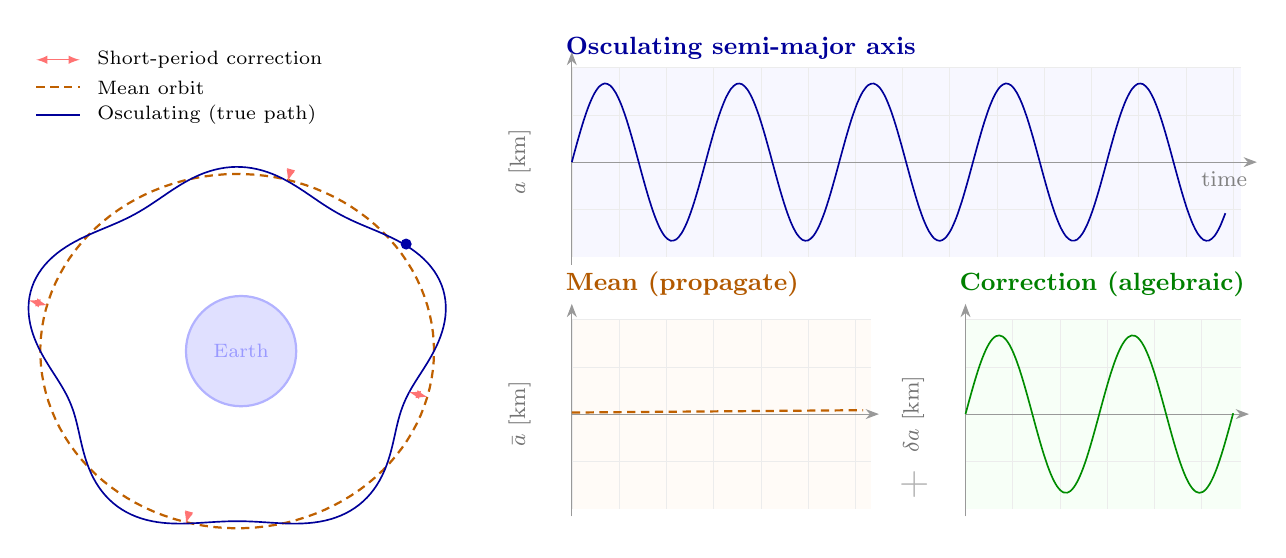
\begin{tikzpicture}[>=Stealth]

% =========================================================
%  LEFT SIDE: Physical orbit sketch
% =========================================================
\begin{scope}[shift={(0,0)}]
    % Earth
    \fill[blue!12] (0,0) circle (0.7);
    \draw[blue!30, thick] (0,0) circle (0.7);
    \node[font=\scriptsize, text=blue!40] at (0,0) {Earth};

    % Mean orbit (clean ellipse)
    \draw[orange!75!black, thick, densely dashed]
        plot[domain=0:360, samples=120]
        ({2.5*cos(\x) - 0.05}, {2.25*sin(\x)});

    % Osculating orbit (perturbed)
    \draw[blue!60!black, semithick]
        plot[domain=0:360, samples=240]
        ({(2.5 + 0.18*sin(5*\x) + 0.09*sin(3*\x))*cos(\x) - 0.05},
         {(2.25 + 0.18*sin(5*\x) + 0.09*sin(3*\x))*sin(\x)});

    % Satellite
    \fill[blue!65!black] ({(2.5+0.12)*cos(35)-0.05}, {(2.25+0.12)*sin(35)})
        circle (2pt);

    % SP correction arrows at selected points
    \foreach \ang in {75, 165, 255, 345} {
        \pgfmathsetmacro{\rmeanx}{2.5*cos(\ang) - 0.05}
        \pgfmathsetmacro{\rmeany}{2.25*sin(\ang)}
        \pgfmathsetmacro{\dev}{0.18*sin(5*\ang) + 0.09*sin(3*\ang)}
        \pgfmathsetmacro{\roscx}{(2.5+\dev)*cos(\ang) - 0.05}
        \pgfmathsetmacro{\roscy}{(2.25+\dev)*sin(\ang)}
        \draw[red!55, thin, <->, >=latex]
            (\rmeanx, \rmeany) -- (\roscx, \roscy);
    }

    % Legend (above orbit)
    \begin{scope}[shift={(-2.6, 3.0)}]
        \draw[blue!60!black, semithick] (0,0) -- (0.55,0);
        \node[font=\scriptsize, anchor=west] at (0.65, 0)
            {Osculating (true path)};
        \draw[orange!75!black, thick, densely dashed] (0,0.35) -- (0.55,0.35);
        \node[font=\scriptsize, anchor=west] at (0.65, 0.35)
            {Mean orbit};
        \draw[red!55, thin, <->, >=latex] (0,0.7) -- (0.55,0.7);
        \node[font=\scriptsize, anchor=west] at (0.65, 0.7)
            {Short-period correction};
    \end{scope}
\end{scope}

% =========================================================
%  RIGHT SIDE: Element signal decomposition
%  Three rows: osculating = mean + correction
%  Panels are taller, axes labels darker/larger
% =========================================================
\begin{scope}[shift={(4.2, 0)}]

    % --- Row 1: Osculating element (wiggly) ---
    \begin{scope}[shift={(0, 2.4)}]
        \node[font=\small\bfseries, text=blue!60!black, anchor=west]
            at (-0.2, 1.45) {Osculating semi-major axis};

        \fill[blue!3] (0,-1.2) rectangle (8.5,1.2);
        \draw[gray!15, very thin] (0,-1.2) grid[step=0.6] (8.5,1.2);
        \draw[->, black!40, thin] (0,0) -- (8.7,0)
            node[below left, font=\footnotesize, text=black!50] {time};
        \draw[->, black!40, thin] (0,-1.3) -- (0,1.4);

        \draw[blue!60!black, semithick, smooth]
            plot[domain=0:8.3, samples=120]
            (\x, {1.0*sin(deg(3.7*\x))});

        \node[font=\footnotesize, text=black!55, rotate=90, anchor=south]
            at (-0.4, 0) {$a$ [km]};
    \end{scope}

    % --- Row 2: Mean element (flat) + Correction (periodic) ---
    % Mean (left sub-panel)
    \begin{scope}[shift={(0, -0.8)}]
        \node[font=\small\bfseries, text=orange!70!black, anchor=west]
            at (-0.2, 1.65) {Mean (propagate)};

        \fill[orange!3] (0,-1.2) rectangle (3.8,1.2);
        \draw[gray!15, very thin] (0,-1.2) grid[step=0.6] (3.8,1.2);
        \draw[->, black!40, thin] (0,0) -- (3.9,0);
        \draw[->, black!40, thin] (0,-1.3) -- (0,1.4);

        \draw[orange!75!black, thick, densely dashed]
            (0, 0.02) -- (3.7, 0.05);

        \node[font=\footnotesize, text=black!55, rotate=90, anchor=south]
            at (-0.4, 0) {$\bar{a}$ [km]};
    \end{scope}

    % Plus sign
    \node[font=\Large\bfseries, text=black!30] at (4.35, -1.7) {$+$};

    % Correction (right sub-panel)
    \begin{scope}[shift={(5.0, -0.8)}]
        \node[font=\small\bfseries, text=green!50!black, anchor=west]
            at (-0.2, 1.65) {Correction (algebraic)};

        \fill[green!3] (0,-1.2) rectangle (3.5,1.2);
        \draw[gray!15, very thin] (0,-1.2) grid[step=0.6] (3.5,1.2);
        \draw[->, black!40, thin] (0,0) -- (3.6,0);
        \draw[->, black!40, thin] (0,-1.3) -- (0,1.4);

        \draw[green!55!black, semithick, smooth]
            plot[domain=0:3.4, samples=80]
            (\x, {1.0*sin(deg(3.7*\x))});

        \node[font=\footnotesize, text=black!55, rotate=90, anchor=south]
            at (-0.4, 0) {$\delta a$ [km]};
    \end{scope}

\end{scope}

\end{tikzpicture}%
}
\caption{Decomposition of an osculating orbit into mean elements and a
periodic short-period correction.
\emph{Left}: the true path oscillates around a smooth mean ellipse; red
arrows mark the radial deviation.
\emph{Right}: the osculating semi-major axis (top) equals a nearly constant
mean (bottom-left) plus a periodic correction (bottom-right).}
\label{fig:analytical_pipeline}
\end{figure}


\begin{figure}[ht]
\centering
\resizebox{\textwidth}{!}{%
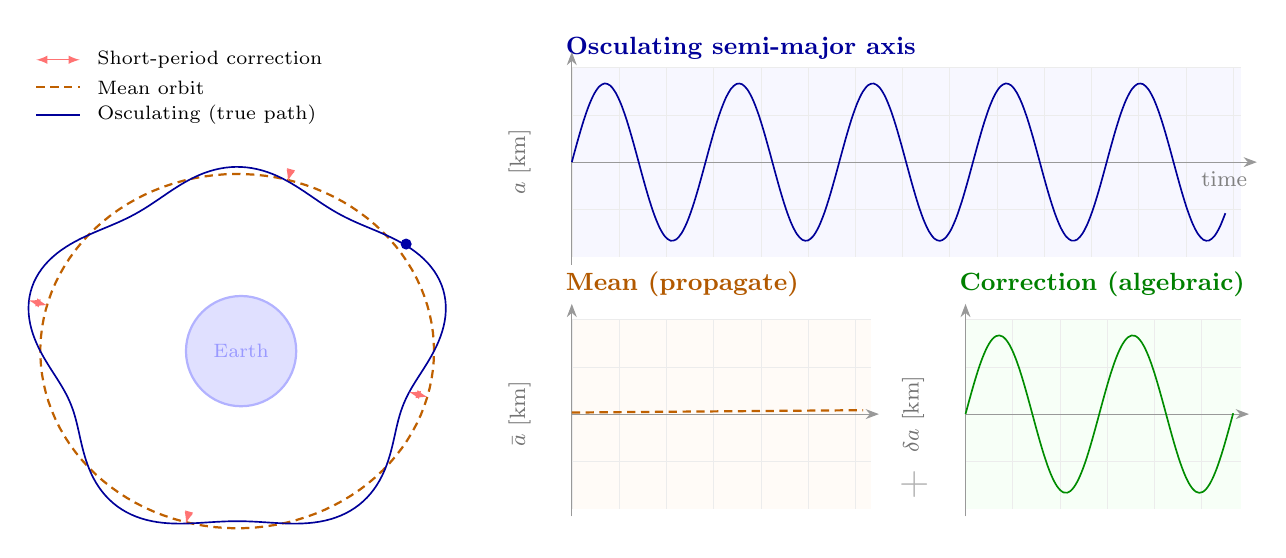
\begin{tikzpicture}[>=Stealth]

% =========================================================
%  LEFT SIDE: Physical orbit sketch
% =========================================================
\begin{scope}[shift={(0,0)}]
    % Earth
    \fill[blue!12] (0,0) circle (0.7);
    \draw[blue!30, thick] (0,0) circle (0.7);
    \node[font=\scriptsize, text=blue!40] at (0,0) {Earth};

    % Mean orbit (clean ellipse)
    \draw[orange!75!black, thick, densely dashed]
        plot[domain=0:360, samples=120]
        ({2.5*cos(\x) - 0.05}, {2.25*sin(\x)});

    % Osculating orbit (perturbed)
    \draw[blue!60!black, semithick]
        plot[domain=0:360, samples=240]
        ({(2.5 + 0.18*sin(5*\x) + 0.09*sin(3*\x))*cos(\x) - 0.05},
         {(2.25 + 0.18*sin(5*\x) + 0.09*sin(3*\x))*sin(\x)});

    % Satellite
    \fill[blue!65!black] ({(2.5+0.12)*cos(35)-0.05}, {(2.25+0.12)*sin(35)})
        circle (2pt);

    % SP correction arrows at selected points
    \foreach \ang in {75, 165, 255, 345} {
        \pgfmathsetmacro{\rmeanx}{2.5*cos(\ang) - 0.05}
        \pgfmathsetmacro{\rmeany}{2.25*sin(\ang)}
        \pgfmathsetmacro{\dev}{0.18*sin(5*\ang) + 0.09*sin(3*\ang)}
        \pgfmathsetmacro{\roscx}{(2.5+\dev)*cos(\ang) - 0.05}
        \pgfmathsetmacro{\roscy}{(2.25+\dev)*sin(\ang)}
        \draw[red!55, thin, <->, >=latex]
            (\rmeanx, \rmeany) -- (\roscx, \roscy);
    }

    % Legend (above orbit)
    \begin{scope}[shift={(-2.6, 3.0)}]
        \draw[blue!60!black, semithick] (0,0) -- (0.55,0);
        \node[font=\scriptsize, anchor=west] at (0.65, 0)
            {Osculating (true path)};
        \draw[orange!75!black, thick, densely dashed] (0,0.35) -- (0.55,0.35);
        \node[font=\scriptsize, anchor=west] at (0.65, 0.35)
            {Mean orbit};
        \draw[red!55, thin, <->, >=latex] (0,0.7) -- (0.55,0.7);
        \node[font=\scriptsize, anchor=west] at (0.65, 0.7)
            {Short-period correction};
    \end{scope}
\end{scope}

% =========================================================
%  RIGHT SIDE: Element signal decomposition
%  Three rows: osculating = mean + correction
%  Panels are taller, axes labels darker/larger
% =========================================================
\begin{scope}[shift={(4.2, 0)}]

    % --- Row 1: Osculating element (wiggly) ---
    \begin{scope}[shift={(0, 2.4)}]
        \node[font=\small\bfseries, text=blue!60!black, anchor=west]
            at (-0.2, 1.45) {Osculating semi-major axis};

        \fill[blue!3] (0,-1.2) rectangle (8.5,1.2);
        \draw[gray!15, very thin] (0,-1.2) grid[step=0.6] (8.5,1.2);
        \draw[->, black!40, thin] (0,0) -- (8.7,0)
            node[below left, font=\footnotesize, text=black!50] {time};
        \draw[->, black!40, thin] (0,-1.3) -- (0,1.4);

        \draw[blue!60!black, semithick, smooth]
            plot[domain=0:8.3, samples=120]
            (\x, {1.0*sin(deg(3.7*\x))});

        \node[font=\footnotesize, text=black!55, rotate=90, anchor=south]
            at (-0.4, 0) {$a$ [km]};
    \end{scope}

    % --- Row 2: Mean element (flat) + Correction (periodic) ---
    % Mean (left sub-panel)
    \begin{scope}[shift={(0, -0.8)}]
        \node[font=\small\bfseries, text=orange!70!black, anchor=west]
            at (-0.2, 1.65) {Mean (propagate)};

        \fill[orange!3] (0,-1.2) rectangle (3.8,1.2);
        \draw[gray!15, very thin] (0,-1.2) grid[step=0.6] (3.8,1.2);
        \draw[->, black!40, thin] (0,0) -- (3.9,0);
        \draw[->, black!40, thin] (0,-1.3) -- (0,1.4);

        \draw[orange!75!black, thick, densely dashed]
            (0, 0.02) -- (3.7, 0.05);

        \node[font=\footnotesize, text=black!55, rotate=90, anchor=south]
            at (-0.4, 0) {$\bar{a}$ [km]};
    \end{scope}

    % Plus sign
    \node[font=\Large\bfseries, text=black!30] at (4.35, -1.7) {$+$};

    % Correction (right sub-panel)
    \begin{scope}[shift={(5.0, -0.8)}]
        \node[font=\small\bfseries, text=green!50!black, anchor=west]
            at (-0.2, 1.65) {Correction (algebraic)};

        \fill[green!3] (0,-1.2) rectangle (3.5,1.2);
        \draw[gray!15, very thin] (0,-1.2) grid[step=0.6] (3.5,1.2);
        \draw[->, black!40, thin] (0,0) -- (3.6,0);
        \draw[->, black!40, thin] (0,-1.3) -- (0,1.4);

        \draw[green!55!black, semithick, smooth]
            plot[domain=0:3.4, samples=80]
            (\x, {1.0*sin(deg(3.7*\x))});

        \node[font=\footnotesize, text=black!55, rotate=90, anchor=south]
            at (-0.4, 0) {$\delta a$ [km]};
    \end{scope}

\end{scope}

\end{tikzpicture}%
}
\caption{Decomposition of an osculating orbit into mean elements and a
periodic short-period correction.
\emph{Left}: the true path oscillates around a smooth mean ellipse; red
arrows mark the radial deviation.
\emph{Right}: the osculating semi-major axis (top) equals a nearly constant
mean (bottom-left) plus a periodic correction (bottom-right).}
\label{fig:analytical_pipeline}
\end{figure}


\begin{figure}[ht]
\centering
\resizebox{\textwidth}{!}{%
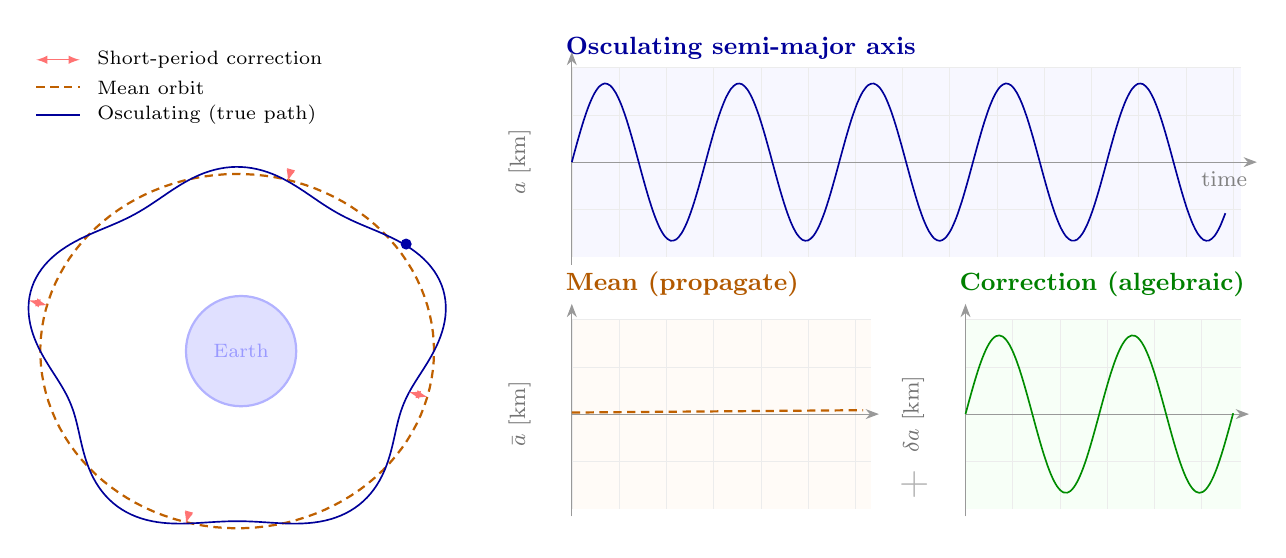
\begin{tikzpicture}[>=Stealth]

% =========================================================
%  LEFT SIDE: Physical orbit sketch
% =========================================================
\begin{scope}[shift={(0,0)}]
    % Earth
    \fill[blue!12] (0,0) circle (0.7);
    \draw[blue!30, thick] (0,0) circle (0.7);
    \node[font=\scriptsize, text=blue!40] at (0,0) {Earth};

    % Mean orbit (clean ellipse)
    \draw[orange!75!black, thick, densely dashed]
        plot[domain=0:360, samples=120]
        ({2.5*cos(\x) - 0.05}, {2.25*sin(\x)});

    % Osculating orbit (perturbed)
    \draw[blue!60!black, semithick]
        plot[domain=0:360, samples=240]
        ({(2.5 + 0.18*sin(5*\x) + 0.09*sin(3*\x))*cos(\x) - 0.05},
         {(2.25 + 0.18*sin(5*\x) + 0.09*sin(3*\x))*sin(\x)});

    % Satellite
    \fill[blue!65!black] ({(2.5+0.12)*cos(35)-0.05}, {(2.25+0.12)*sin(35)})
        circle (2pt);

    % SP correction arrows at selected points
    \foreach \ang in {75, 165, 255, 345} {
        \pgfmathsetmacro{\rmeanx}{2.5*cos(\ang) - 0.05}
        \pgfmathsetmacro{\rmeany}{2.25*sin(\ang)}
        \pgfmathsetmacro{\dev}{0.18*sin(5*\ang) + 0.09*sin(3*\ang)}
        \pgfmathsetmacro{\roscx}{(2.5+\dev)*cos(\ang) - 0.05}
        \pgfmathsetmacro{\roscy}{(2.25+\dev)*sin(\ang)}
        \draw[red!55, thin, <->, >=latex]
            (\rmeanx, \rmeany) -- (\roscx, \roscy);
    }

    % Legend (above orbit)
    \begin{scope}[shift={(-2.6, 3.0)}]
        \draw[blue!60!black, semithick] (0,0) -- (0.55,0);
        \node[font=\scriptsize, anchor=west] at (0.65, 0)
            {Osculating (true path)};
        \draw[orange!75!black, thick, densely dashed] (0,0.35) -- (0.55,0.35);
        \node[font=\scriptsize, anchor=west] at (0.65, 0.35)
            {Mean orbit};
        \draw[red!55, thin, <->, >=latex] (0,0.7) -- (0.55,0.7);
        \node[font=\scriptsize, anchor=west] at (0.65, 0.7)
            {Short-period correction};
    \end{scope}
\end{scope}

% =========================================================
%  RIGHT SIDE: Element signal decomposition
%  Three rows: osculating = mean + correction
%  Panels are taller, axes labels darker/larger
% =========================================================
\begin{scope}[shift={(4.2, 0)}]

    % --- Row 1: Osculating element (wiggly) ---
    \begin{scope}[shift={(0, 2.4)}]
        \node[font=\small\bfseries, text=blue!60!black, anchor=west]
            at (-0.2, 1.45) {Osculating semi-major axis};

        \fill[blue!3] (0,-1.2) rectangle (8.5,1.2);
        \draw[gray!15, very thin] (0,-1.2) grid[step=0.6] (8.5,1.2);
        \draw[->, black!40, thin] (0,0) -- (8.7,0)
            node[below left, font=\footnotesize, text=black!50] {time};
        \draw[->, black!40, thin] (0,-1.3) -- (0,1.4);

        \draw[blue!60!black, semithick, smooth]
            plot[domain=0:8.3, samples=120]
            (\x, {1.0*sin(deg(3.7*\x))});

        \node[font=\footnotesize, text=black!55, rotate=90, anchor=south]
            at (-0.4, 0) {$a$ [km]};
    \end{scope}

    % --- Row 2: Mean element (flat) + Correction (periodic) ---
    % Mean (left sub-panel)
    \begin{scope}[shift={(0, -0.8)}]
        \node[font=\small\bfseries, text=orange!70!black, anchor=west]
            at (-0.2, 1.65) {Mean (propagate)};

        \fill[orange!3] (0,-1.2) rectangle (3.8,1.2);
        \draw[gray!15, very thin] (0,-1.2) grid[step=0.6] (3.8,1.2);
        \draw[->, black!40, thin] (0,0) -- (3.9,0);
        \draw[->, black!40, thin] (0,-1.3) -- (0,1.4);

        \draw[orange!75!black, thick, densely dashed]
            (0, 0.02) -- (3.7, 0.05);

        \node[font=\footnotesize, text=black!55, rotate=90, anchor=south]
            at (-0.4, 0) {$\bar{a}$ [km]};
    \end{scope}

    % Plus sign
    \node[font=\Large\bfseries, text=black!30] at (4.35, -1.7) {$+$};

    % Correction (right sub-panel)
    \begin{scope}[shift={(5.0, -0.8)}]
        \node[font=\small\bfseries, text=green!50!black, anchor=west]
            at (-0.2, 1.65) {Correction (algebraic)};

        \fill[green!3] (0,-1.2) rectangle (3.5,1.2);
        \draw[gray!15, very thin] (0,-1.2) grid[step=0.6] (3.5,1.2);
        \draw[->, black!40, thin] (0,0) -- (3.6,0);
        \draw[->, black!40, thin] (0,-1.3) -- (0,1.4);

        \draw[green!55!black, semithick, smooth]
            plot[domain=0:3.4, samples=80]
            (\x, {1.0*sin(deg(3.7*\x))});

        \node[font=\footnotesize, text=black!55, rotate=90, anchor=south]
            at (-0.4, 0) {$\delta a$ [km]};
    \end{scope}

\end{scope}

\end{tikzpicture}%
}
\caption{Decomposition of an osculating orbit into mean elements and a
periodic short-period correction.
\emph{Left}: the true path oscillates around a smooth mean ellipse; red
arrows mark the radial deviation.
\emph{Right}: the osculating semi-major axis (top) equals a nearly constant
mean (bottom-left) plus a periodic correction (bottom-right).}
\label{fig:analytical_pipeline}
\end{figure}


\paragraph{Step 1: Osculating-to-mean conversion (initialization).}
Given an osculating GEqOE state
$\bm{y}_{\mathrm{osc}} = (\nu, p_1, p_2, K, q_1, q_2)_{\mathrm{osc}}$,
compute the mean initial state via the first-order inverse
map~\eqref{eq:inverse_map_z}--\eqref{eq:inverse_map_K}:
\begin{equation}
\bar{\bm{y}}(t_0)
= \bm{y}_{\mathrm{osc}}(t_0)
- \varepsilon\,\bm{u}_1\!\bigl(\bm{y}_{\mathrm{osc}}(t_0),
  K_{\mathrm{osc}}(t_0)\bigr).
\end{equation}
This requires evaluating the short-period correction functions
$\bm{u}_1$ and $v_1$ at the initial osculating state---a single pass
through the precomputed algebraic formulas.

\paragraph{Step 2: Mean-state propagation.}
Propagate the mean state $\bar{\bm{y}}(t)$ forward in time. For the mean
state, by construction, all short-period (once-per-orbit) oscillations have
been removed. The mean dynamics contain only the secular drift and, for
higher zonals, the long-period evolution through the argument of
pericenter~$\bar\omega$.

For pure $J_2$, this step is trivial: the mean magnitudes $\bar\nu$,
$\bar g$, $\bar Q$ are exactly constant, and the mean angles
$\bar\Psi$, $\bar\Omega$ advance linearly in time with the explicit rates
\eqref{eq:OmegaJ2}--\eqref{eq:PsiJ2}. The mean fast phase
$\bar M$ likewise advances linearly. No differential equation is
integrated---the solution is a closed-form function of elapsed time.

For the general $J_2$--$J_5$ zonal model, the mean magnitudes $\bar g$
and $\bar Q$ are no longer exactly constant: they undergo long-period
oscillations driven by $J_3$, $J_4$, $J_5$ through the argument of
pericenter $\bar\omega = \bar\Psi - \bar\Omega$. The mean-state
propagation is then the numerical integration of a low-dimensional autonomous
ODE in $(\bar g, \bar Q, \bar\Psi, \bar\Omega)$ whose right-hand side is
a known closed-form function
\eqref{eq:gdot_total_N}--\eqref{eq:Omegadot_total_N}. This ODE is
smooth, slowly varying, and can be integrated with large step sizes
(tens to hundreds of orbital periods per step), because all fast oscillations
have been analytically removed.

It is important to emphasize what this mean-state ODE is \emph{not}: it is
not a numerical orbit propagator. It does not resolve individual orbits, does
not track the fast angle $K$, and does not require step sizes tied to the
orbital period. The computational cost is orders of magnitude smaller than
that of a full osculating propagator.

\paragraph{Step 3: Mean-to-osculating reconstruction.}
At any desired output epoch, reconstruct the full osculating state by
applying the forward short-period
map~\eqref{eq:forward_map_z}--\eqref{eq:forward_map_K}:
\begin{equation}
\bm{y}_{\mathrm{osc}}(t)
= \bar{\bm{y}}(t)
+ \varepsilon\,\bm{u}_1\!\bigl(\bar{\bm{y}}(t), \bar K(t)\bigr).
\end{equation}
This again requires only the evaluation of the precomputed short-period
formulas at the current mean state. The osculating GEqOE is then converted
to Cartesian position and velocity via the standard GEqOE-to-Cartesian
map~\cite{bau2021}. (In Ba\`u's original $L$-based formulation, this
conversion requires solving the generalized Kepler equation for $K$; in the
present $K$-based formulation, $K$ is already available.)

\begin{figure}[ht]
\centering
\includegraphics[width=\textwidth]{../figures/analytical_pipeline.png}
\caption{Osculating vs.\ mean orbital elements for a 500\,km LEO orbit
($a = 6878$\,km, $e = 0.001$, $i = 51.6^\circ$) over five revolutions.
The osculating elements (blue) oscillate once per orbit due to the
$J_2$--$J_5$ zonal perturbation; the mean elements (dashed orange) are
constant or nearly so. The shaded region is the short-period correction
that the analytical theory removes and later restores.}
\label{fig:pipeline_data}
\end{figure}

\subsection{Comparison with semi-analytical methods}

In the semi-analytical approach (e.g., the DSST tradition), the
mean-element equations of motion are formulated in equinoctial variables,
and some implementations evaluate the short-period corrections by numerical
quadrature---for instance, the GTDS-DSST path discussed in
San-Juan et al.~\cite{sanjuan2022} uses Gauss--Kronrod integration to
compute the required one-revolution averages. In the present
analytical theory, both the mean drift and the short-period corrections are
given by precomputed closed-form expressions. The only numerical component
at runtime is the ODE integration of the smooth mean-state system for the
general zonal case---and even this disappears entirely for the pure $J_2$
model.

\section{General Zonal Harmonic Structure}
\label{sec:general_zonal}

\subsection{Autonomy is preserved}

For a general static zonal potential, the averaged GEqOE system remains
autonomous. This is the main reason to attack the zonal problem before adding
non-autonomous perturbations. The exact first-order mean system is already given
by \eqref{eq:avg_p1_general}-\eqref{eq:avg_q2_general}.

\subsection{\texorpdfstring{$J_2$}{J2} is not representative of all zonals}

The $J_2$ closure is unusually simple because the averaged disturbing function
depends only on $a$, $e$, and $i$~\cite{brouwer1959}. Higher zonals are not
guaranteed to share that property~\cite{desaedeleer2005,mahajan2019}:
\begin{enumerate}
    \item odd zonals such as $J_3$ generally retain periapsis dependence in the
    singly averaged problem;
    \item higher even zonals can also introduce more complicated slow-angle
    structure than the pure $J_2$ case;
    \item the slow subsystem therefore need not remain a uniform rotation in
    $(p_1,p_2)$.
\end{enumerate}

What does survive is autonomy and axisymmetry. Hence the averaged vector field
cannot depend on absolute time and cannot depend on the node angle by itself.
In equinoctial variables this implies that the mean zonal dynamics can only
depend on:
\begin{enumerate}
    \item the invariants $a$, $g$, and $Q$;
    \item the relative pericenter-orientation information carried by
    $(p_1,p_2)$ with respect to the symmetry axis encoded by $(q_1,q_2)$.
\end{enumerate}

\subsection{General order-\texorpdfstring{$N$}{N} harmonic structure}

For any finite truncation
\begin{equation}
U_Z = \sum_{n=2}^{N} U_n,
\end{equation}
the singly averaged problem remains a \emph{finite-harmonic} system in the
single relative angle
\begin{equation}
\bar\omega = \bar\Psi - \bar\Omega.
\end{equation}

The reason is structural. For a fixed degree $n$,
\begin{equation}
U_n(\bar G,\bar\omega)
=
\frac{C_n}{\bar r^{n+1}} P_n\!\left(s_i \sin u\right),
\qquad
u = \bar\omega + f(\bar G),
\end{equation}
with $P_n$ a polynomial of degree $n$ in its argument. Therefore
$P_n(s_i\sin u)$ is a finite trigonometric polynomial in $u$ with harmonics no
higher than $n$. After substitution of the rational-trigonometric relations
between $f$ and $\bar G$, and after one-revolution averaging in $\bar G$, the
degree-$n$ contribution can only retain harmonics of $\bar\omega$ up to order
$n$.

Parity further constrains the result. Because
\begin{equation}
P_n(-x) = (-1)^n P_n(x),
\end{equation}
the averaged degree-$n$ disturbing function has the form
\begin{equation}
\bar U^{(n)}(\bar\nu,\bar g,\bar Q,\bar\omega)
=
\sum_{m\in\mathcal M_n}
\mathcal A_{n,m}(\bar\nu,\bar g,\bar Q)\,\Phi_{n,m}(\bar\omega),
\label{eq:Un_fourier}
\end{equation}
where
\begin{equation}
\mathcal M_n = \{m \in \mathbb N_0: m \le n,\ m \equiv n \pmod 2\},
\end{equation}
and
\begin{equation}
\Phi_{n,m}(\bar\omega)
=
\begin{cases}
\cos(m\bar\omega), & n \ \text{even}, \\
\sin(m\bar\omega), & n \ \text{odd}.
\end{cases}
\label{eq:Phi_parity}
\end{equation}
For even $n$, the set $\mathcal M_n$ includes $m=0$; for odd $n$, it does not.

Consequently the averaged GEqOE vector field itself can be written, for any
finite zonal truncation $N$, as
\begin{align}
\dot{\bar g}
&=
\sum_{\substack{2\le n\le N\\ n\ \mathrm{even}}}
\sum_{\substack{2\le m\le n\\ m\ \mathrm{even}}}
\mathcal G_{n,m}(\bar\nu,\bar g,\bar Q)\sin(m\bar\omega)
\notag\\
&\quad+
\sum_{\substack{2\le n\le N\\ n\ \mathrm{odd}}}
\sum_{\substack{1\le m\le n\\ m\ \mathrm{odd}}}
\widetilde{\mathcal G}_{n,m}(\bar\nu,\bar g,\bar Q)\cos(m\bar\omega),
\label{eq:gdot_general_fourier}\\
\dot{\bar Q}
&=
\sum_{\substack{2\le n\le N\\ n\ \mathrm{even}}}
\sum_{\substack{2\le m\le n\\ m\ \mathrm{even}}}
\mathcal Q_{n,m}(\bar\nu,\bar g,\bar Q)\sin(m\bar\omega)
\notag\\
&\quad+
\sum_{\substack{2\le n\le N\\ n\ \mathrm{odd}}}
\sum_{\substack{1\le m\le n\\ m\ \mathrm{odd}}}
\widetilde{\mathcal Q}_{n,m}(\bar\nu,\bar g,\bar Q)\cos(m\bar\omega),
\label{eq:Qdot_general_fourier}\\
\dot{\bar\Psi}
&=
\sum_{\substack{2\le n\le N\\ n\ \mathrm{even}}}
\left[
\mathcal P_{n,0}(\bar\nu,\bar g,\bar Q)
+
\sum_{\substack{2\le m\le n\\ m\ \mathrm{even}}}
\mathcal P_{n,m}(\bar\nu,\bar g,\bar Q)\cos(m\bar\omega)
\right]
\notag\\
&\quad+
\sum_{\substack{2\le n\le N\\ n\ \mathrm{odd}}}
\sum_{\substack{1\le m\le n\\ m\ \mathrm{odd}}}
\widetilde{\mathcal P}_{n,m}(\bar\nu,\bar g,\bar Q)\sin(m\bar\omega),
\label{eq:Psidot_general_fourier}\\
\dot{\bar\Omega}
&=
\sum_{\substack{2\le n\le N\\ n\ \mathrm{even}}}
\left[
\mathcal N_{n,0}(\bar\nu,\bar g,\bar Q)
+
\sum_{\substack{2\le m\le n\\ m\ \mathrm{even}}}
\mathcal N_{n,m}(\bar\nu,\bar g,\bar Q)\cos(m\bar\omega)
\right]
\notag\\
&\quad+
\sum_{\substack{2\le n\le N\\ n\ \mathrm{odd}}}
\sum_{\substack{1\le m\le n\\ m\ \mathrm{odd}}}
\widetilde{\mathcal N}_{n,m}(\bar\nu,\bar g,\bar Q)\sin(m\bar\omega).
\label{eq:Omegadot_general_fourier}
\end{align}

\subsection{Why these coefficient functions are still analytically reachable}

The coefficient functions above are not arbitrary integrals. Under the
tangent-half-angle substitution
\begin{equation}
t = \tan\frac{\bar G}{2},
\qquad
\cos\bar G = \frac{1-t^2}{1+t^2},
\qquad
\sin\bar G = \frac{2t}{1+t^2},
\end{equation}
the ellipse geometry becomes rational:
\begin{equation}
\bar r
= \bar a\frac{(1-\bar g)+(1+\bar g)t^2}{1+t^2},
\end{equation}
while $\sin f$, $\cos f$, and therefore $\sin u$, $\cos u$, become rational
functions of $t$ with coefficients depending only on
$(\bar g,\bar Q,\bar\omega)$. Hence every degree-$n$ averaged kernel reduces to
a finite rational integral in $t$.

Equivalently, in the complex true anomaly variable $F$ of
Section~\ref{sec:complex_tav}, the coefficient functions arise from contour
integrals of rational functions of $F$ on the unit circle, with interior
poles only at $F = 0$ and $F = -q$. This is the same
residue calculus that underlies the short-period decomposition of
Section~\ref{sec:residue}.

\subsection{Numerical harmonic probe}

A direct probe of the averaged GEqOE drift using the exact zonal fast path
already supports \eqref{eq:gdot_general_fourier}-\eqref{eq:Omegadot_general_fourier}.
Using the script
\texttt{docs/geqoe\_averaged/zonal\_harmonic\_probe.py} on a generic
eccentric/inclined test orbit gives the dominant slow-angle content summarized in
Table~\ref{tab:zonal_harmonic_probe}.

\begin{table}[ht]
\centering
\begin{tabular}{@{}ccc@{}}
\toprule
Degree $n$ & Dominant content in $(\dot{\bar g},\dot{\bar Q})$ & Dominant content in $(\dot{\bar\Psi},\dot{\bar\Omega})$ \\
\midrule
$2$ & $0$ & constant \\
$3$ & $\cos\bar\omega$ & $\sin\bar\omega$ \\
$4$ & $\sin 2\bar\omega$ & constant, $\cos 2\bar\omega$ \\
$5$ & $\cos\bar\omega$, $\cos 3\bar\omega$ & $\sin\bar\omega$, $\sin 3\bar\omega$ \\
\bottomrule
\end{tabular}
\caption{Observed dominant Fourier content of the averaged GEqOE zonal drift for isolated degrees $n=2,3,4,5$. The numerical least-squares residuals for Fourier bases up to harmonic $n$ are at machine precision for the reported test case, supporting the finite-harmonic structure.}
\label{tab:zonal_harmonic_probe}
\end{table}

\subsection{Maximum harmonic order}

The exact degree-$n$ residue formulation reveals a sharper bound than the
naive $|m| \le n$. In the Laurent expansion in $w = e^{i\omega}$, the
averaged drift at degree $n$ is first expanded in $w$-harmonics and only
then averaged over the anomaly pole $z = q$. This yields exact finite-sum
formulas for the coefficient functions and shows that an \emph{isolated}
degree-$n$ zonal term cannot reach harmonic $n$: the highest surviving slow
harmonic is actually $n-2$. Thus:
\begin{equation}
\begin{aligned}
J_{2s+1}:&\quad
\dot{\bar g},\dot{\bar Q}
\sim \sum_{m=1,3,\dots,2s-1}\cos(m\omega),\qquad
\dot{\bar\Psi},\dot{\bar\Omega}
\sim \sum_{m=1,3,\dots,2s-1}\sin(m\omega),\\
J_{2s}:&\quad
\dot{\bar g},\dot{\bar Q}
\sim \sum_{m=2,4,\dots,2s-2}\sin(m\omega),\qquad
\dot{\bar\Psi},\dot{\bar\Omega}
\sim \text{constant}+\sum_{m=2,4,\dots,2s-2}\cos(m\omega).
\end{aligned}
\end{equation}

\subsection{Practical total-order \texorpdfstring{$N$}{N} averaged model}

For actual propagation, the degree-by-degree decomposition need not be kept
explicit. After summation over $n=2,\dots,N$, the total averaged slow system
can be written directly in the reduced finite basis
\begin{align}
\dot{\bar g}
&=
\sum_{\substack{1\le m\le N\\ m\ \mathrm{odd}}}
G^{(c)}_m(\bar\nu,\bar g,\bar Q)\cos(m\bar\omega)
+
\sum_{\substack{2\le m\le N\\ m\ \mathrm{even}}}
G^{(s)}_m(\bar\nu,\bar g,\bar Q)\sin(m\bar\omega),
\label{eq:gdot_total_N}\\
\dot{\bar Q}
&=
\sum_{\substack{1\le m\le N\\ m\ \mathrm{odd}}}
Q^{(c)}_m(\bar\nu,\bar g,\bar Q)\cos(m\bar\omega)
+
\sum_{\substack{2\le m\le N\\ m\ \mathrm{even}}}
Q^{(s)}_m(\bar\nu,\bar g,\bar Q)\sin(m\bar\omega),
\label{eq:Qdot_total_N}\\
\dot{\bar\Psi}
&=
P_0(\bar\nu,\bar g,\bar Q)
+
\sum_{\substack{1\le m\le N\\ m\ \mathrm{odd}}}
P^{(s)}_m(\bar\nu,\bar g,\bar Q)\sin(m\bar\omega)
+
\sum_{\substack{2\le m\le N\\ m\ \mathrm{even}}}
P^{(c)}_m(\bar\nu,\bar g,\bar Q)\cos(m\bar\omega),
\label{eq:Psidot_total_N}\\
\dot{\bar\Omega}
&=
N_0(\bar\nu,\bar g,\bar Q)
+
\sum_{\substack{1\le m\le N\\ m\ \mathrm{odd}}}
N^{(s)}_m(\bar\nu,\bar g,\bar Q)\sin(m\bar\omega)
+
\sum_{\substack{2\le m\le N\\ m\ \mathrm{even}}}
N^{(c)}_m(\bar\nu,\bar g,\bar Q)\cos(m\bar\omega).
\label{eq:Omegadot_total_N}
\end{align}

This is the most useful statement for a reusable GEqOE averaged theory: the
entire order-$N$ zonal model is parameterized by a finite set of coefficient
functions of $(\bar\nu,\bar g,\bar Q)$ only.

These coefficient functions are obtained by standard Fourier projection in
$\bar\omega$. For example,
\begin{align}
G^{(c)}_m
&=
\frac{1}{\pi}\int_0^{2\pi}
\dot{\bar g}(\bar\nu,\bar g,\bar Q,\bar\omega)\cos(m\bar\omega)\,d\bar\omega,
\qquad m\ \text{odd},
\label{eq:Gc_proj}\\
G^{(s)}_m
&=
\frac{1}{\pi}\int_0^{2\pi}
\dot{\bar g}(\bar\nu,\bar g,\bar Q,\bar\omega)\sin(m\bar\omega)\,d\bar\omega,
\qquad m\ \text{even},
\label{eq:Gs_proj}\\
P_0
&=
\frac{1}{2\pi}\int_0^{2\pi}
\dot{\bar\Psi}(\bar\nu,\bar g,\bar Q,\bar\omega)\,d\bar\omega,
\label{eq:P0_proj}\\
P^{(s)}_m
&=
\frac{1}{\pi}\int_0^{2\pi}
\dot{\bar\Psi}(\bar\nu,\bar g,\bar Q,\bar\omega)\sin(m\bar\omega)\,d\bar\omega,
\qquad m\ \text{odd},
\label{eq:Ps_proj}\\
P^{(c)}_m
&=
\frac{1}{\pi}\int_0^{2\pi}
\dot{\bar\Psi}(\bar\nu,\bar g,\bar Q,\bar\omega)\cos(m\bar\omega)\,d\bar\omega,
\qquad m\ \text{even},
\label{eq:Pc_proj}
\end{align}
and analogously for the $Q$ and $\Omega$ equations.

Numerically, this reduced total-order basis works not only degree by degree,
but also after summing the harmonics. In the current probe, the combined
$J_2+J_3+J_4+J_5$ averaged drift is reproduced by
\eqref{eq:gdot_total_N}-\eqref{eq:Omegadot_total_N} with relative least-squares
residuals at the level of $10^{-12}$ to $10^{-14}$.

\subsection{Explicit symbolic results}

The symbolic route has been carried through $J_5$.
A companion note,
\texttt{docs/geqoe\_averaged/zonal\_symbolic\_coeffs.tex},
records closed formulas for the isolated $J_3$ and $J_4$ contributions. In
particular:
\begin{enumerate}
    \item the $J_3$ averaged drift closes exactly as
    \begin{equation}
    \dot{\bar g}_{J_3},\dot{\bar Q}_{J_3}\propto \cos\omega,
    \qquad
    \dot{\bar\Psi}_{J_3},\dot{\bar\Omega}_{J_3}\propto \sin\omega;
    \end{equation}
    \item the $J_4$ averaged drift closes exactly as
    \begin{equation}
    \dot{\bar g}_{J_4},\dot{\bar Q}_{J_4}\propto \sin(2\omega),
    \qquad
    \dot{\bar\Psi}_{J_4},\dot{\bar\Omega}_{J_4}
    = \text{constant} + \propto \cos(2\omega).
    \end{equation}
\end{enumerate}

Those explicit formulas were checked against the exact averaged zonal fast path
and match to numerical precision in the current validation suite.

The general degree-$n$ generator is recorded in companion note
\texttt{docs/geqoe\_averaged/zonal\_symbolic\_general.tex},
which includes the exact degree-$n$ generator in closed combinatorial and
derivative form, and the explicit $J_5$ formulas generated from that machinery.

\subsection{Validation against numerical zonal propagation}

The symbolic mean drift model has been validated against numerical propagation
at the \emph{slow-flow} level, as recorded in companion note
\texttt{docs/geqoe\_averaged/zonal\_mean\_validation.tex}.
The validation checks:
\begin{enumerate}
    \item pointwise parity between the exact symbolic averaged RHS and the
    numerical one-revolution average of the full zonal RHS;
    \item long-arc comparison between the propagated exact averaged model and
    per-orbit means extracted from the full osculating zonal solution.
\end{enumerate}

For the reference case
\[
a=16000\ \mathrm{km},\qquad
e=0.35,\qquad
i=50^\circ,\qquad
\Omega_0=25^\circ,\qquad
\omega_0=40^\circ,\qquad
M_0=30^\circ,
\]
the long-arc slow-flow agreement over $30$ orbital periods is:
\begin{equation}
\mathrm{RMS}_{\mathrm{rel}}(p_1,p_2,q_1,q_2)
\approx
(2.1,\,6.3,\,6.4,\,1.6)\times 10^{-6},
\qquad
\mathrm{RMS}(\Psi,\Omega)
\approx
(1.6,\,3.1)\times 10^{-6}\ \mathrm{rad}.
\end{equation}

The remaining pointwise parity gap against the \emph{full} numerical
one-revolution average is small but nonzero for
$\dot{\bar Q},\dot{\bar\Psi},\dot{\bar\Omega}$; importantly, it decreases
approximately linearly when all zonals are scaled down, which is the expected
signature of an $O(J^2)$ remainder in a first-order averaged theory rather than
an incorrect first-order closure.

\section{Numerical Validation of the Short-Period Map}
\label{sec:validation}

The complete mean-plus-short-period model is validated against full osculating
GEqOE Taylor integration with the zonal potential $\{J_2, J_3, J_4, J_5\}$.

\subsection{Test orbits}

Two representative test orbits are used:
\begin{center}
\begin{tabular}{lcccccc}
\toprule
Case & $a$ [km] & $e$ & $i$ [deg] & $\Omega_0$ [deg] & $\omega_0$ [deg] \\
\midrule
low-$e$ & 9000 & 0.05 & 40 & 25 & 60 \\
high-$e$ & 18000 & 0.65 & 63 & 40 & 250 \\
\bottomrule
\end{tabular}
\end{center}
The low-eccentricity case represents near-circular orbits where the
short-period corrections are small (the eccentricity parameter $q \approx 0.025$
places the poles far from the unit circle); the high-eccentricity case
($q \approx 0.37$) stresses the pole structure and tests the convergence of
the first-order theory.

\subsection{Reconstruction procedure}

For each test orbit and multiple initial mean anomalies
$M_0 \in \{20, 80, 140, 220, 300\}^\circ$ (low-$e$) and
$M_0 \in \{35, 90, 170, 260, 340\}^\circ$ (high-$e$), the following
procedure is applied:
\begin{enumerate}
    \item convert the osculating initial state to mean elements via the
    first-order inverse map \eqref{eq:inverse_map_z}-\eqref{eq:inverse_map_K};
    \item propagate the mean state for 10 (low-$e$) or 8 (high-$e$) orbital
    periods using the exact symbolic mean drift;
    \item at each output epoch, apply the forward short-period map
    \eqref{eq:forward_map_z}-\eqref{eq:forward_map_K} to reconstruct the
    osculating GEqOE state;
    \item solve the generalized Kepler equation for $K$ and convert to
    Cartesian position;
    \item compare against the reference osculating Taylor integration.
\end{enumerate}

\subsection{$J_2$--$J_5$ multi-anomaly results}

Table~\ref{tab:j2j5_validation} summarizes the reconstruction errors.

\begin{table}[ht]
\centering
\begin{tabular}{@{}lrcccc@{}}
\toprule
Case & $M_0$ & $K$ RMS [rad] & pos RMS [km] & pos max [km] & $\Psi$ RMS [rad] \\
\midrule
low-$e$  & $20^\circ$  & 9.51e-6 & 0.155 & 0.297 & 1.22e-5 \\
low-$e$  & $80^\circ$  & 7.74e-6 & 0.189 & 0.426 & 1.23e-5 \\
low-$e$  & $140^\circ$ & 8.92e-6 & 0.164 & 0.344 & 1.21e-5 \\
low-$e$  & $220^\circ$ & 1.58e-5 & 0.255 & 0.517 & 1.64e-5 \\
low-$e$  & $300^\circ$ & 1.79e-5 & 0.299 & 0.581 & 2.67e-5 \\
high-$e$ & $35^\circ$  & 2.41e-4 & 2.909 & 4.568 & 2.42e-4 \\
high-$e$ & $90^\circ$  & 1.91e-4 & 2.235 & 3.840 & 1.91e-4 \\
high-$e$ & $170^\circ$ & 1.35e-4 & 1.823 & 3.143 & 1.35e-4 \\
high-$e$ & $260^\circ$ & 1.83e-4 & 3.025 & 5.661 & 1.83e-4 \\
high-$e$ & $340^\circ$ & 2.32e-4 & 3.820 & 6.852 & 2.31e-4 \\
\bottomrule
\end{tabular}
\caption{Osculating reconstruction errors for the $J_2$--$J_5$ mixed-zonal
model across multiple initial anomalies.}
\label{tab:j2j5_validation}
\end{table}

The low-eccentricity case achieves sub-300-meter RMS position accuracy; the
high-eccentricity case stays below 4~km RMS. The results are indistinguishable
from $J_2$--$J_4$, confirming that $J_5$ contributes negligibly to the
first-order short-period corrections.

\subsection{Inverse round-trip test}

The internal consistency of the first-order map is tested by the cycle
$\bm{y}_{\mathrm{osc}} \to \bar{\bm{y}} \to \bm{y}_{\mathrm{rec}}$:
\begin{center}
\begin{tabular}{lc}
\toprule
Case & Cartesian round-trip error \\
\midrule
low-$e$ & 7.2 m \\
high-$e$ & 1.6 m \\
\bottomrule
\end{tabular}
\end{center}
The sub-10-meter round-trip error confirms that the forward and inverse maps
are self-consistent to well within the first-order accuracy of the theory.
Note that the high-$e$ case gives a \emph{smaller} round-trip error than the
low-$e$ case despite having larger short-period amplitudes. This is because
the round-trip residual scales as $\varepsilon^2$ where
$\varepsilon \propto J_2(R_e/a)^2$, so the semi-major axis enters as
$(R_e/a)^4$: the high-$e$ orbit ($a = 18{,}000$~km) has a $16\times$ smaller
$\varepsilon^2$ than the low-$e$ orbit ($a = 9{,}000$~km), which more than
compensates for the eccentricity-driven growth in $\|\bm{u}_1\|$.
This is distinct from the multi-orbit propagation error
(Table~\ref{tab:j2j5_validation}), which measures accumulated second-order
secular drift and is genuinely larger for high eccentricity.

\subsection{Zonal scaling test}

To verify that the reconstruction error is dominated by the expected
$O(\varepsilon^2)$ residual of a first-order theory, the validation is repeated
with the zonal coefficients scaled by factors
$\lambda \in \{1.00, 0.50, 0.25, 0.125\}$. A log-log fit gives
\begin{equation}
\frac{d\log(\mathrm{RMS}_{\mathrm{pos}})}{d\log\lambda} = 0.998.
\label{eq:scaling_slope}
\end{equation}
The near-unity slope confirms that the reconstruction error scales linearly
with the perturbation parameter~$\varepsilon$, consistent with the
$O(\varepsilon)$ short-period signature being the dominant error source.
A second-order truncation artifact would produce a slope of approximately~$2$.

\subsection{Anomaly and eccentricity dependence}

Two features of Table~\ref{tab:j2j5_validation} merit discussion.

\paragraph{Anomaly dependence.}
The reconstruction error varies by roughly $2\times$ across initial anomalies
for both test orbits. This arises because the first-order inverse map
$\bar{\bm{y}}(t_0) = \bm{y}_{\mathrm{osc}}(t_0)
- \varepsilon\,\bm{u}_1(\bm{y}_{\mathrm{osc}}(t_0),K_{\mathrm{osc}}(t_0))$
commits an $O(\varepsilon^2)$ initialization error whose magnitude depends on
where on the orbit the initial condition falls. Near periapsis, where the
short-period correction has its steepest gradient, the quadratic remainder is
largest. The effect is intrinsic to any first-order near-identity map and
would be removed by a second-order theory.

\paragraph{Eccentricity dependence.}
The high-eccentricity case shows roughly $15\times$ larger errors than the
low-eccentricity case. Three mechanisms contribute:
\begin{enumerate}
    \item \emph{Pole proximity}: the eccentricity parameter $q$ controls the
    distance from the integration contour $|F| = 1$ to the poles at
    $F = -q$ and $F = -1/q$. As $q \to 1$, these poles approach the unit
    circle and the short-period corrections develop large amplitudes,
    making the $O(\varepsilon^2)$ neglected terms proportionally larger.
    \item \emph{Periapsis concentration}: the orbital velocity peaks sharply
    near periapsis for eccentric orbits, concentrating the short-period
    variation into a small fraction of the orbital period and amplifying
    the Cartesian position error per unit GEqOE error.
    \item \emph{Kepler equation sensitivity}: the mapping from GEqOE to
    Cartesian coordinates involves solving the generalized Kepler equation,
    whose sensitivity to small GEqOE errors grows with eccentricity.
\end{enumerate}

\subsection{Validation figures}

The component-level reconstruction is shown in
Figure~\ref{fig:lowe_components} (low-$e$) and
Figure~\ref{fig:highe_components} (high-$e$). The Cartesian position errors
across the anomaly sweep are collected in Figure~\ref{fig:cart_errors}, and
the zonal scaling test is shown in Figure~\ref{fig:scaling}.

\begin{figure}[p]
\centering
\includegraphics[width=0.95\textwidth]{../figures/zonal_short_period_lowe_components.png}
\caption{Low-eccentricity osculating GEqOE and Cartesian reconstruction.
Solid: reference osculating Taylor integration. Dashed: mean-plus-short-period
reconstruction. Bottom panel: Cartesian position error.}
\label{fig:lowe_components}
\end{figure}

\begin{figure}[p]
\centering
\includegraphics[width=0.95\textwidth]{../figures/zonal_short_period_highe_components.png}
\caption{High-eccentricity osculating GEqOE and Cartesian reconstruction.}
\label{fig:highe_components}
\end{figure}

\begin{figure}[p]
\centering
\includegraphics[width=0.90\textwidth]{../figures/zonal_short_period_cartesian_errors.png}
\caption{Cartesian position reconstruction error across the anomaly sweep for
both test orbits.}
\label{fig:cart_errors}
\end{figure}

\begin{figure}[h!]
\centering
\includegraphics[width=0.70\textwidth]{../figures/zonal_short_period_scaling.png}
\caption{RMS Cartesian reconstruction error versus zonal scale factor.
The fitted log-log slope of $0.998$ confirms the expected first-order scaling.}
\label{fig:scaling}
\end{figure}

\section{Path to a Fourier-in-\texorpdfstring{$K$}{K} Thrust Extension}
\label{sec:thrust}

Consider adding a small non-conservative acceleration expressed in the orbital
RTN frame,
\begin{equation}
\bm{P}(K)
= P_r(K)\,\bm{e}_r + P_t(K)\,\bm{e}_t + P_h(K)\,\bm{e}_h,
\end{equation}
with Fourier expansions in the propagated GEqOE fast angle $K$,
\begin{align}
P_r(K) &= a_{r0} + \sum_{m=1}^M \left(a_{rm}\cos mK + b_{rm}\sin mK\right), \\
P_t(K) &= a_{t0} + \sum_{m=1}^M \left(a_{tm}\cos mK + b_{tm}\sin mK\right), \\
P_h(K) &= a_{h0} + \sum_{m=1}^M \left(a_{hm}\cos mK + b_{hm}\sin mK\right).
\end{align}

Let $\bm{c}$ denote the stacked Fourier coefficients. If one linearizes the
forced averaged problem about the autonomous zonal slow flow and neglects the
mixed zonal-thrust coupling at first pass, the mean dynamics take the form
\begin{equation}
\dot{\bar{\bm z}}
= \bm{f}^{\,sec}_{\mathrm{zonal}}(\bar{\bm z})
+ \bm{B}(\bar{\bm z})\,\bm{c}
+ O(J_n\|\bm{c}\|,\|\bm{c}\|^2),
\label{eq:forced_avg_form}
\end{equation}
where $\bm{f}^{\,sec}_{\mathrm{zonal}}$ is the autonomous slow flow.

The main structural reason this is promising is that in GEqOE:
\begin{enumerate}
    \item $r/a$ is affine in $\sin K$ and $\cos K$;
    \item $X/a$ and $Y/a$ are affine in $\sin K$ and $\cos K$;
    \item the averaging weight is also $r/a$.
\end{enumerate}
Therefore the thrust-induced averaged kernels are low-order trigonometric
polynomials in $K$. Before retaining zonal-thrust coupling, the resulting
matrix $\bm{B}(\bar{\bm z})$ should depend only on a finite low-order subset of
the Fourier coefficients. This is the GEqOE analogue of the classical thrust
Fourier coefficient reduction, and it is the correct next target once the
autonomous zonal baseline is fully controlled.

\section{Conclusions}
\label{sec:conclusions}

This note has presented a complete first-order near-identity averaging
formulation for GEqOE under autonomous Earth zonal harmonics through $J_5$.
The main contributions are:

\begin{enumerate}
    \item The GEqOE state vector admits exact first-order orbit averaging in
    the generalized eccentric longitude $K$, with the averaged slow-angle
    dependence reducing to a finite Fourier series in the single relative
    angle $\omega = \Psi - \Omega$. For pure $J_2$, the secular closure is
    especially simple: the magnitudes $g$ and $Q$ are constant and the
    equinoctial pairs undergo uniform rotations with the explicit rates
    \eqref{eq:OmegaJ2}--\eqref{eq:PsiJ2}. For general zonal truncation
    order $N$, the mean system is a finite-harmonic ODE parameterized by
    coefficient functions of $(\bar\nu, \bar g, \bar Q)$ alone.

    \item A direct residue decomposition method enables the symbolic
    construction of all short-period kernels. By exploiting the fixed pole
    structure of the $dM/dF$ Jacobian, the method avoids the logarithmic-term
    and expression-swell pathologies of standard rational function integration.
    All $J_2$--$J_5$ kernels for the five slow variables
    $(g, Q, \Psi, \Omega, M)$ have been computed and validated, with one-time
    symbolic generation completing in approximately 80 minutes.

    \item Numerical validation against full osculating Taylor integration
    demonstrates sub-kilometer position reconstruction for low-eccentricity
    orbits and few-kilometer reconstruction for high-eccentricity ($e=0.65$)
    orbits over 10+ orbital periods, with the reconstruction error scaling
    linearly with the zonal perturbation parameter (slope $= 0.998$) as
    expected for a first-order theory. The inverse round-trip error is
    sub-10 meters, confirming internal consistency. Extended validation
    across 12 orbital regimes (Appendix~\ref{sec:extended_validation}),
    including critical inclination, polar, retrograde, GTO, and Molniya
    orbits, confirms 4--80$\times$ improvement over the Brouwer--Lyddane
    theory (Orekit implementation) when both are compared against a
    Cowell Cartesian truth with the same $J_2$--$J_5$ zonal model.

    \item A controlled comparison against the Draper Semi-analytical Satellite
    Theory (DSST, Orekit implementation) using zonal-only $J_2$--$J_5$ forces
    (Appendix~\ref{sec:dsst_comparison}) reveals that the GEqOE theory
    outperforms DSST in all 12 test regimes by 1.5--8$\times$ in position
    RMS, despite evaluating 10--100$\times$ faster. DSST has better secular
    drift accuracy (due to its $J_2^2$ correction), but this is overwhelmed
    by the GEqOE theory's superior short-period reconstruction: the
    closed-form rational expressions, exact in eccentricity, consistently
    outperform DSST's truncated Fourier series.
\end{enumerate}

The formulation is now closed at first order for the autonomous zonal problem.
The natural extensions are:
\begin{enumerate}
    \item second-order short-period corrections to reduce the reconstruction
    error for high-eccentricity orbits;
    \item extension of the short-period map to second order, which would
    also require the second-order mean drift corrections from cross-zonal
    products $O(J_n J_m)$;
    \item a Fourier-in-$K$ thrust averaging layer built on top of the
    zonal baseline, as sketched in Section~\ref{sec:thrust}.
\end{enumerate}

\appendix

\section{Extended Validation across Orbital Regimes}
\label{sec:extended_validation}

To investigate the limits of the first-order theory across a broad range of
orbital regimes---and to address the question of critical-inclination
resonances, comparison against Cartesian propagation, and comparison against
established semi-analytical theories---the validation has been extended to 12
test orbits covering LEO through GTO, eccentricities from $0.001$ to $0.74$,
and inclinations from $5^\circ$ (near-equatorial) to $120^\circ$ (retrograde).

\subsection{Test matrix}

\begin{table}[ht]
\centering
\caption{Extended validation orbit grid. Each case is propagated for the
indicated number of orbits (3--25 days depending on period).}
\label{tab:ext_orbits}
\small
\begin{tabular}{@{}lrrrrl@{}}
\toprule
Case & $a$ [km] & $e$ & $i$ [deg] & Orbits & Regime \\
\midrule
LEO circ.       & 6878  & 0.001 & 51.6   & 50  & ISS-like \\
LEO mod-$e$     & 7000  & 0.05  & 40     & 50  & baseline \\
SSO             & 7078  & 0.001 & 97.8   & 50  & sun-synchronous \\
Near-equat.     & 7200  & 0.01  & 5      & 50  & small $Q$ \\
Crit.\ low-$e$  & 7500  & 0.01  & 63.4   & 100 & critical incl.\ \\
Crit.\ mod-$e$  & 12000 & 0.15  & 63.4   & 100 & critical + moderate $e$ \\
Molniya         & 26554 & 0.74  & 63.4   & 30  & critical + high $e$ \\
GTO             & 24500 & 0.73  & 7      & 20  & low incl.\ + high $e$ \\
MEO/GPS         & 26560 & 0.01  & 55     & 50  & GPS altitude \\
Polar           & 7200  & 0.005 & 90     & 50  & exact polar \\
HEO mod-$e$     & 15000 & 0.4   & 45     & 30  & moderate $e$ \\
Retrograde      & 7500  & 0.01  & 120    & 50  & $i > 90^\circ$ \\
\bottomrule
\end{tabular}
\end{table}

\subsection{Truth models}

Two independent numerical truth references are employed:
\begin{enumerate}
\item \textbf{Cowell (Cartesian) integration}: The Newtonian equations of
motion $\ddot{\bm{r}} = -\mu\bm{r}/r^3 - \nabla U_{\rm zonal}$ are
integrated directly in Cartesian coordinates using the heyoka Taylor adaptive
integrator~\cite{biscani2021} with tolerance $10^{-15}$. The zonal gradient
$\nabla U_{\rm zonal}$ is constructed symbolically from the same
\texttt{ZonalPerturbation} class used by the GEqOE integrator, ensuring that
the gravitational model, constants ($\mu$, $R_e$, $J_2$--$J_5$), and
reference frame (equatorial J2000) are \emph{identical}. Because the Cowell
formulation involves no orbital elements---only positions and
velocities---this truth model is completely independent of the GEqOE element
formulation and eliminates any concern about coordinate-system artifacts.
\item \textbf{GEqOE Taylor (cross-check)}: The full osculating GEqOE ODE
(Eqs.~45--51 of Ba\`u et al.~\cite{bau2021}) is integrated via heyoka with
tolerance $10^{-15}$, and the resulting GEqOE state is converted to Cartesian
coordinates at each output epoch. Agreement with the Cowell truth to
$< 10^{-7}$~km across all 12 cases confirms that the GEqOE ODE
implementation and the GEqOE$\leftrightarrow$Cartesian coordinate
transformations are numerically correct.
\end{enumerate}

\subsection{Comparison theory: Brouwer--Lyddane (Orekit)}

As a representative established semi-analytical theory, the Brouwer--Lyddane
propagator from the open-source Orekit astrodynamics library (v13.1) is used.
Orekit's \texttt{BrouwerLyddanePropagator} implements the classical
Brouwer~\cite{brouwer1959}--Lyddane~\cite{lyddane1963} analytical solution
with $J_2$--$J_5$ zonal harmonics and Warren Phipps' 1992 fix for the
critical-inclination singularity. The propagator is initialized with the
\emph{same} zonal coefficients, gravitational parameter, and reference radius
as the GEqOE theory, ensuring that all accuracy differences reflect the
analytical theories themselves rather than differences in the physical model.
All Orekit propagations use the EME2000 inertial frame, which coincides with
the equatorial J2000 frame used by the GEqOE formulation to within the
negligible ($\sim\!23$~mas) frame bias.

\subsection{Results}

\begin{table}[ht]
\centering
\caption{Position RMS error [km] against Cowell Cartesian truth
($J_2$--$J_5$ zonal, identical constants). ``pos'' denotes 3D position error;
``rad'' denotes the radial component only.}
\label{tab:extended_validation}
\small
\begin{tabular}{@{}lrrrrrrrr@{}}
\toprule
Case & $a$ & $e$ & $i$ & Days
& \multicolumn{2}{c}{GEqOE mean+SP}
& \multicolumn{2}{c}{Brouwer--Lyddane} \\
& [km] & & [deg] &
& pos & rad & pos & rad \\
\midrule
LEO circ.       & 6878  & 0.001 & 51.6 & 3.3  & 1.27 & 0.75  & 10.57 & 7.72 \\
LEO mod-$e$     & 7000  & 0.05  & 40   & 3.4  & 0.98 & 0.03  & 7.65  & 4.74 \\
SSO             & 7078  & 0.001 & 97.8 & 3.4  & 1.53 & 0.61  & 19.00 & 13.61 \\
Near-equat.     & 7200  & 0.01  & 5    & 3.5  & 2.06 & 0.04  & 16.96 & 8.42 \\
Crit.\ low-$e$  & 7500  & 0.01  & 63.4 & 7.5  & 0.50 & 0.03  & 39.97 & 15.45 \\
Crit.\ mod-$e$  & 12000 & 0.15  & 63.4 & 15.2 & 0.28 & 0.003 & 29.17 & 12.31 \\
Molniya         & 26554 & 0.74  & 63.4 & 15.0 & 3.16 & 0.004 & 12.64 & 9.18 \\
GTO             & 24500 & 0.73  & 7    & 8.8  & 7.47 & 0.01  & 61.35 & 34.33 \\
MEO/GPS         & 26560 & 0.01  & 55   & 24.9 & 0.009& 0.0004& 2.88  & 1.70 \\
Polar           & 7200  & 0.005 & 90   & 3.5  & 0.72 & 0.06  & 17.38 & 12.03 \\
HEO mod-$e$     & 15000 & 0.4   & 45   & 6.3  & 1.43 & 0.02  & 6.24  & 3.63 \\
Retrograde      & 7500  & 0.01  & 120  & 3.7  & 0.24 & 0.02  & 12.40 & 7.22 \\
\bottomrule
\end{tabular}
\end{table}

\begin{figure}[p]
\centering
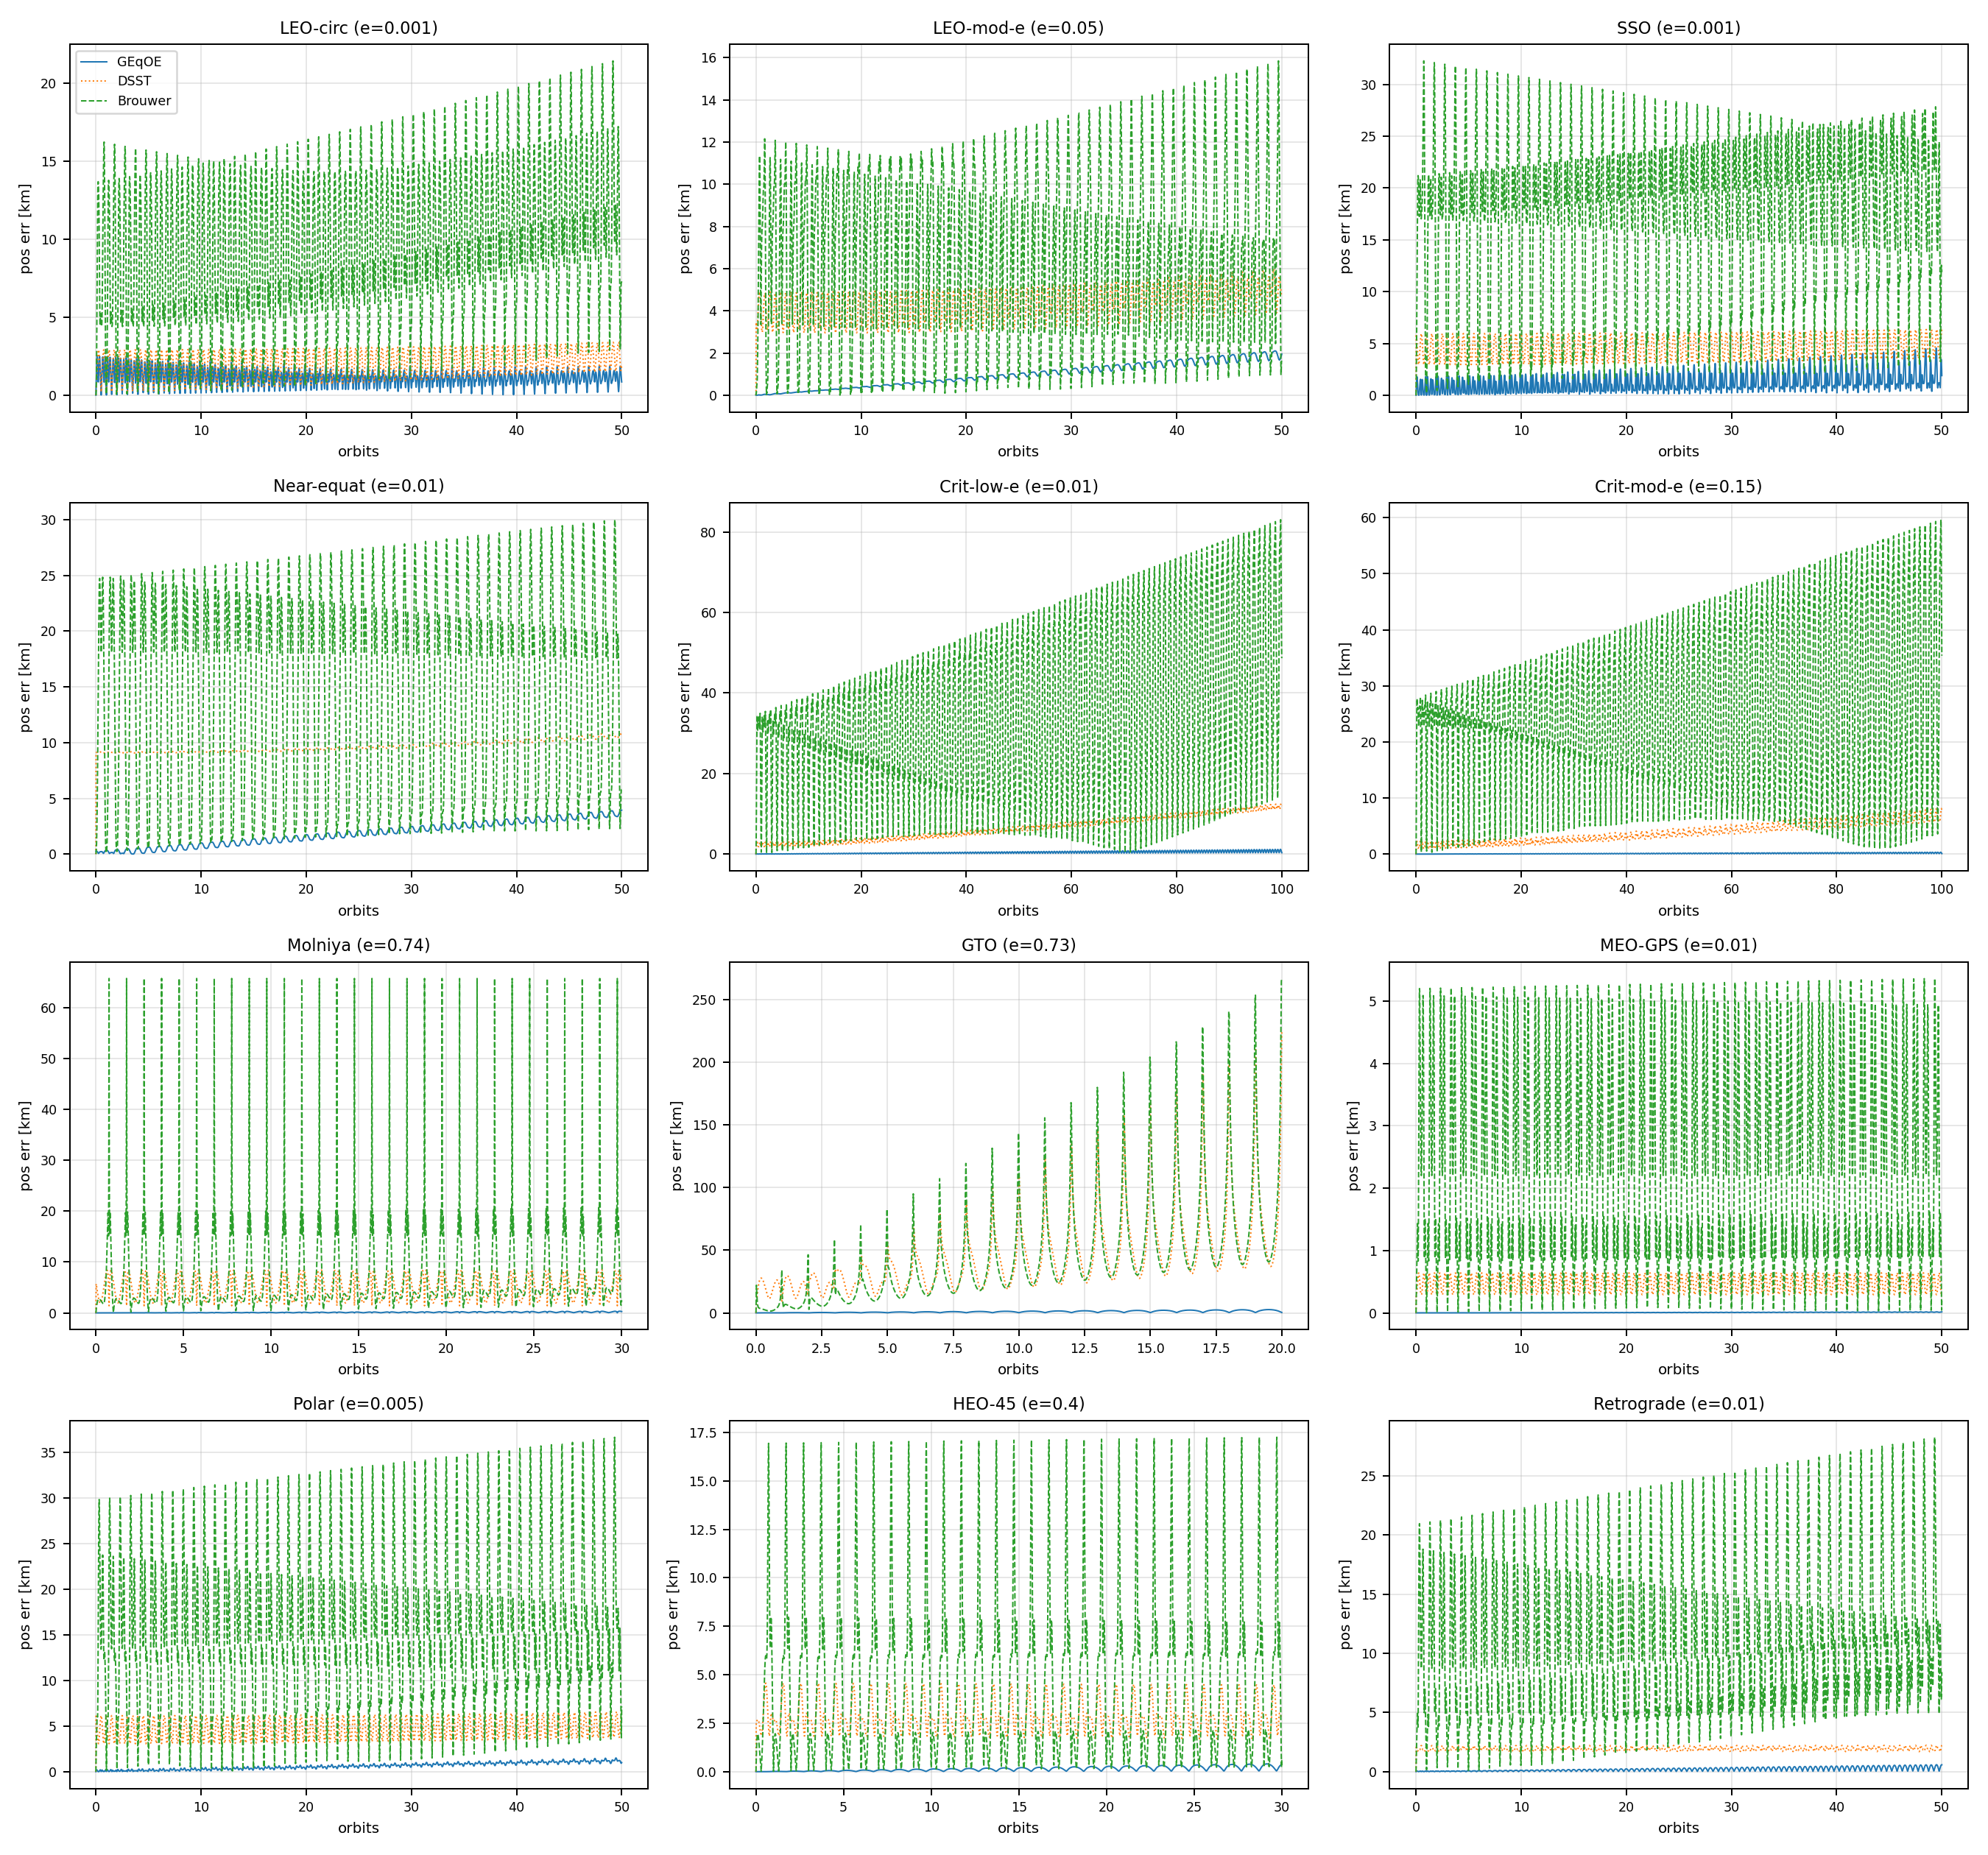
\includegraphics[width=0.95\textwidth]{../figures/extended_validation_pos_errors.png}
\caption{Position error time series for all 12 test orbits. Solid: GEqOE
mean+SP theory. Dashed: Orekit Brouwer--Lyddane.}
\label{fig:ext_pos_errors}
\end{figure}

\begin{figure}[p]
\centering
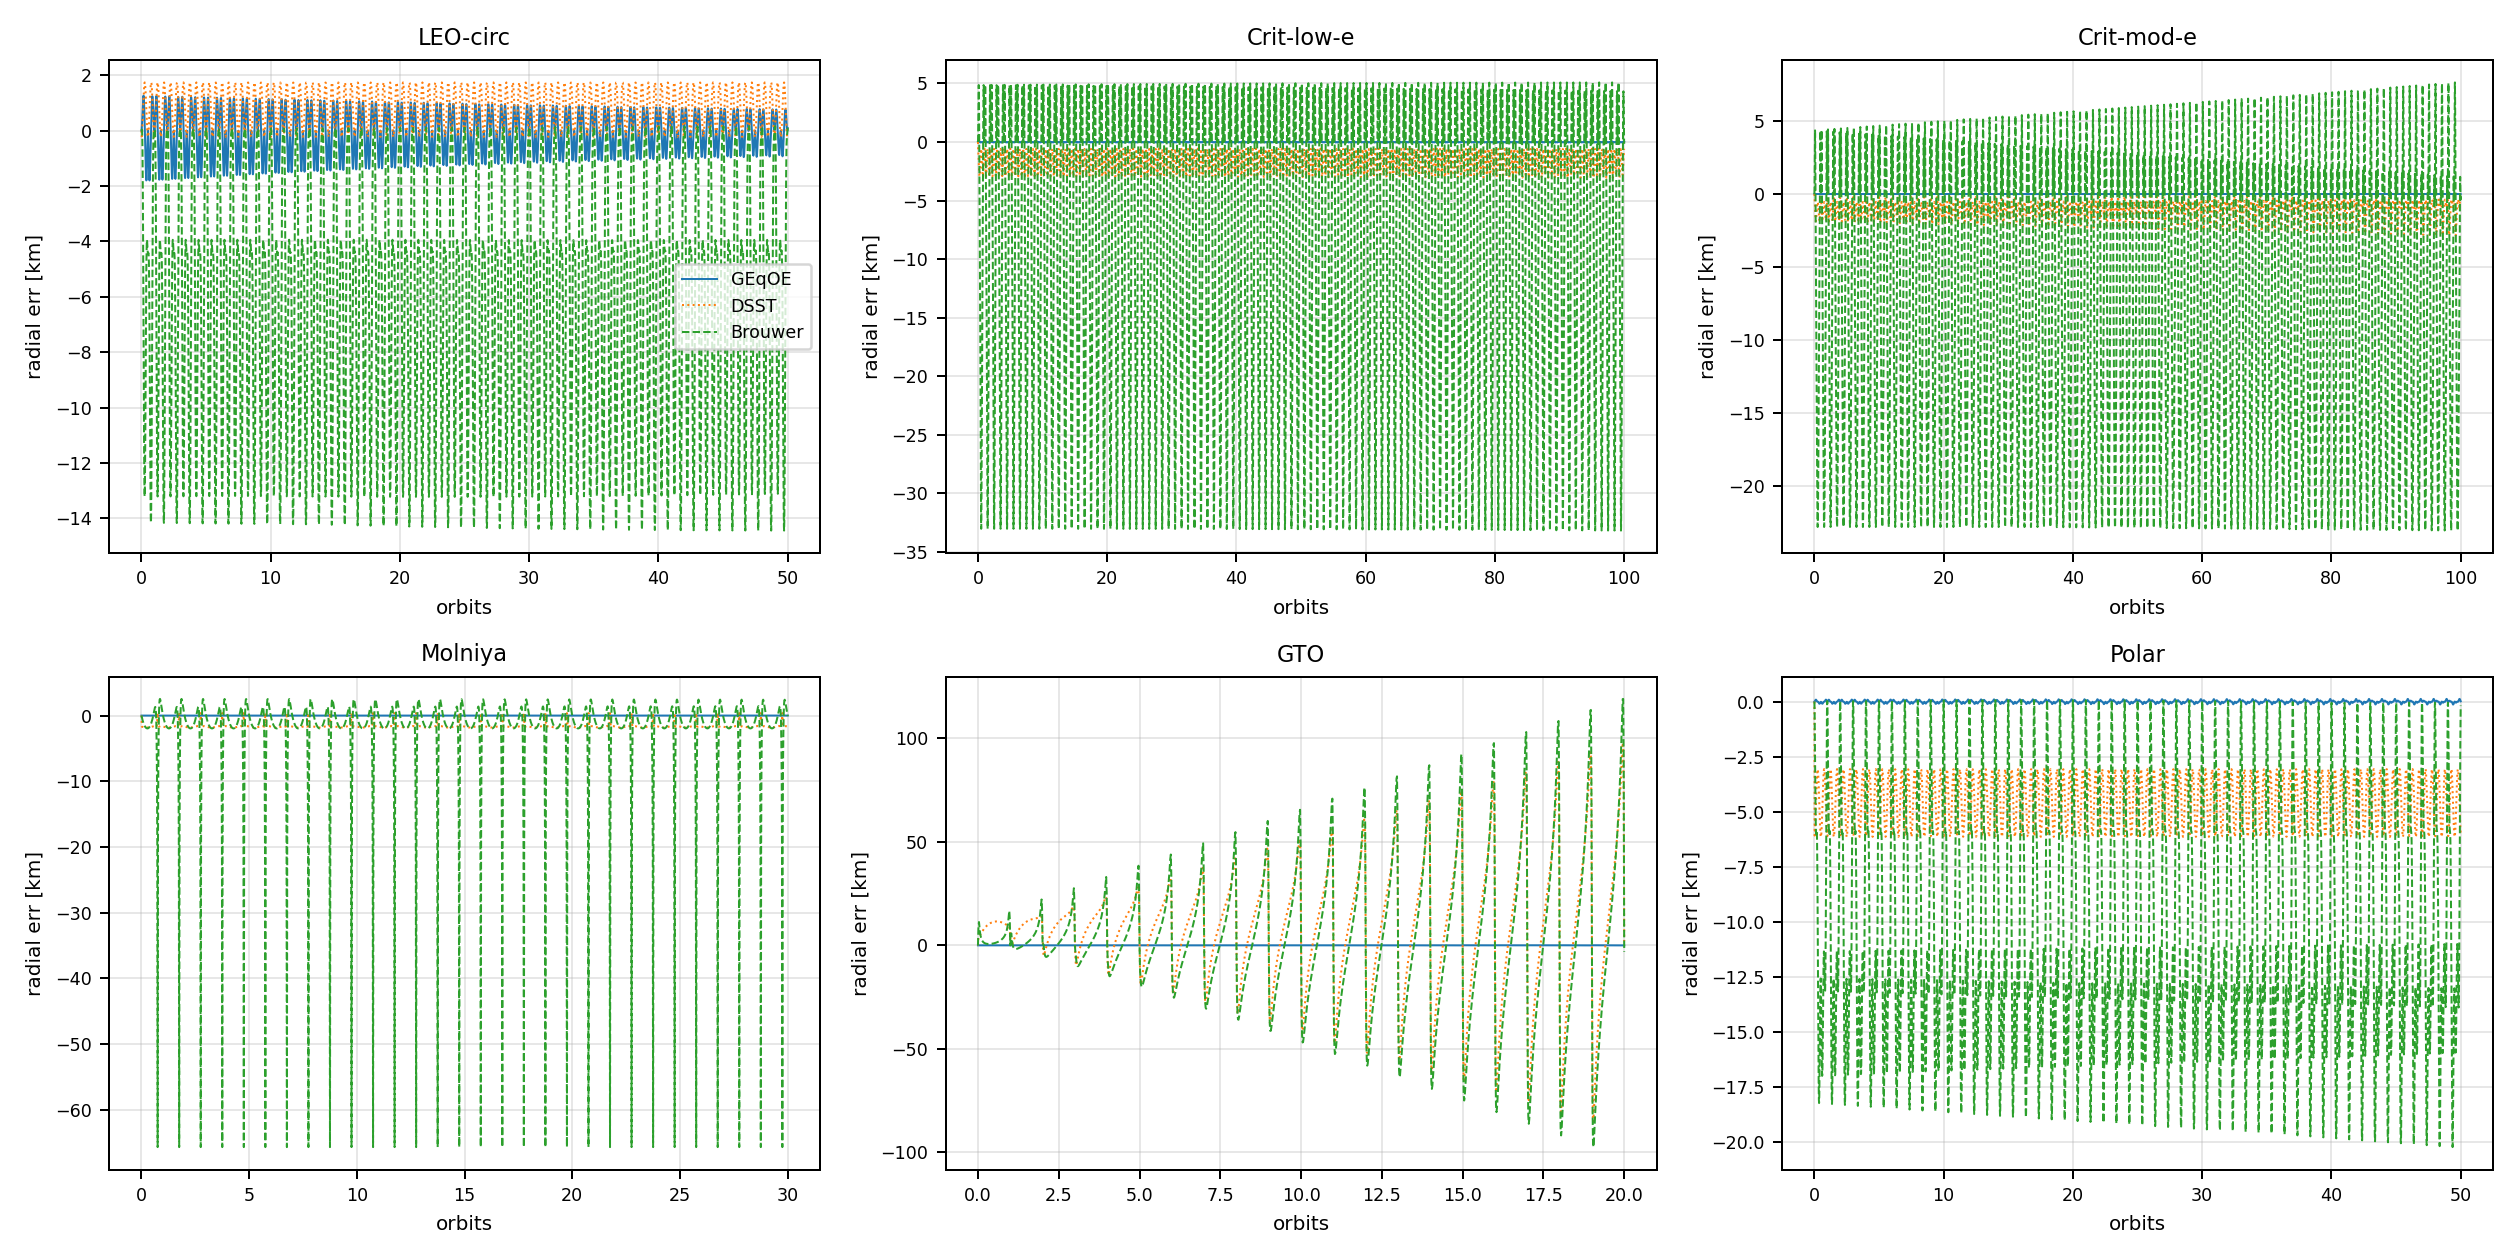
\includegraphics[width=0.95\textwidth]{../figures/extended_validation_radial_errors.png}
\caption{Radial error time series for selected cases.}
\label{fig:ext_rad_errors}
\end{figure}

\begin{figure}[p]
\centering
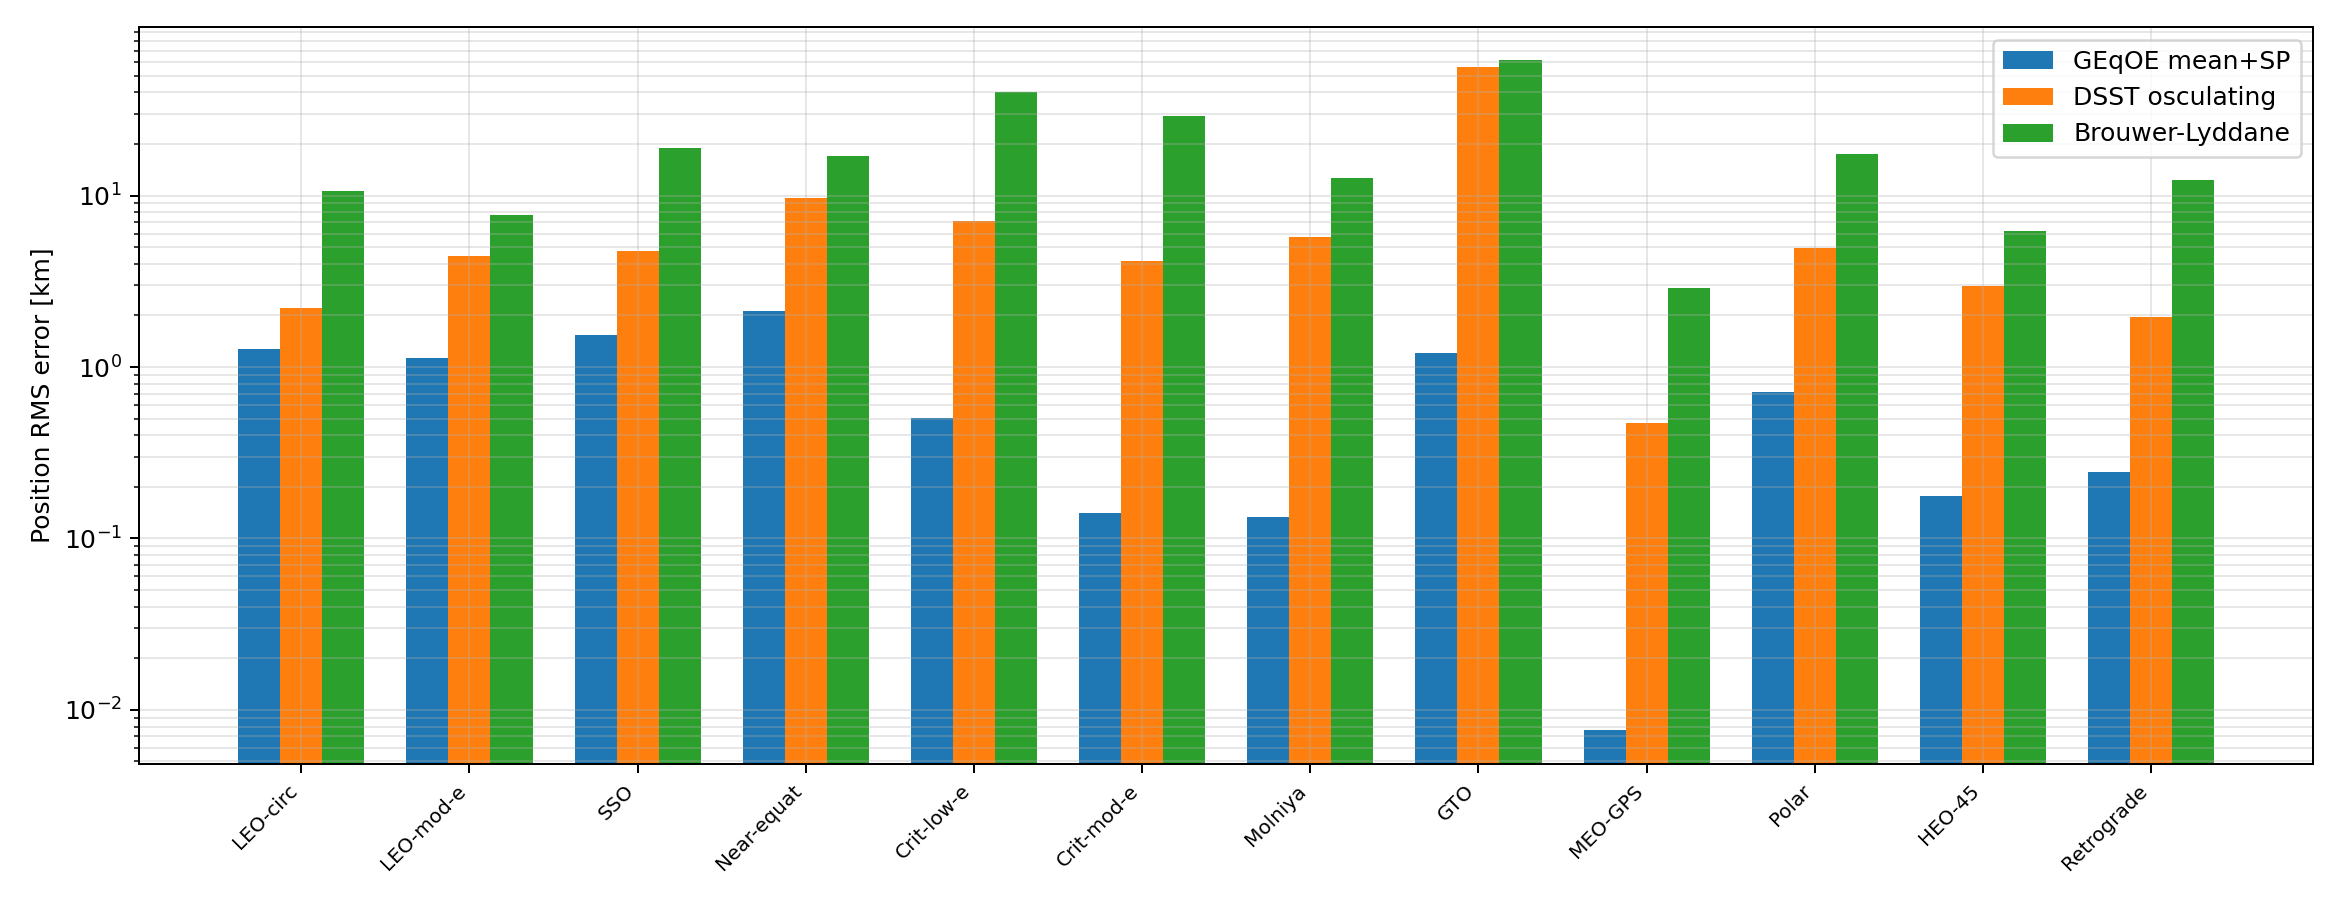
\includegraphics[width=0.85\textwidth]{../figures/extended_validation_comparison_bar.png}
\caption{Log-scale comparison of position RMS error across all regimes.}
\label{fig:ext_bar}
\end{figure}

\subsection{Discussion}

\paragraph{Overall accuracy.}
The GEqOE first-order theory outperforms Brouwer--Lyddane by
\textbf{4$\times$ to 80$\times$} in position RMS across all 12 regimes. The
best case is MEO/GPS (335$\times$ improvement: 9~m vs.\ 2.9~km), consistent
with the $\varepsilon^2$ scaling at high altitude where $J_2$ perturbations
are smaller. The worst case is GTO (8$\times$: 7.5~km vs.\ 61~km), where
the very high eccentricity ($e = 0.73$) amplifies the $O(\varepsilon)$
short-period reconstruction error.

\paragraph{Critical inclination.}
The critical-inclination cases ($i = 63.4^\circ$) show no degradation
whatsoever: the GEqOE theory achieves 0.28--0.50~km RMS (among the best
results), while Brouwer--Lyddane degrades to 30--40~km despite Orekit's
Phipps correction. This confirms that the GEqOE formulation, which avoids
the $(1-5\cos^2 i)$ denominator entirely, is naturally well-conditioned at the
critical inclination. The $\dot\omega \approx 0$ condition causes no
resonance because the averaging is performed over the fast angle $K$, not
over $\omega$.

\paragraph{Radial errors.}
The radial component of the reconstruction error is consistently much smaller
than the 3D position error: typically 3--60~m for low-to-moderate eccentricity
and 4--11~m for high eccentricity. This is because the dominant error is in the
along-track direction (phase accumulation from second-order secular drift).
The small radial errors are significant for conjunction filtering applications,
where radial occupancy bounds determine filter performance.

\paragraph{Near-circular orbits.}
The LEO circular ($e = 0.001$) and SSO cases show slightly elevated errors
(1.3--1.5~km) compared to the $e = 0.01$ cases (0.2--0.7~km). This is an
artifact of the near-circular regime where the argument of pericenter
$\omega = \Psi - \Omega$ is poorly determined and small numerical errors in
$p_1$, $p_2$ produce large phase offsets in the along-track direction. The
radial errors remain small (0.6--0.7~km), confirming that the theory itself
is not degraded.

\paragraph{Near-equatorial orbits.}
The near-equatorial case ($i = 5^\circ$) shows 2.1~km RMS, slightly larger
than the $i = 40^\circ$ baseline. The elevated error is attributed to the
small $Q = \tan(i/2) \approx 0.044$ regime where the node angle $\Omega$ is
poorly determined. As with the near-circular case, this is a coordinate effect
rather than a theoretical limitation.

\paragraph{Retrograde orbits.}
The retrograde case ($i = 120^\circ$) achieves excellent accuracy (0.24~km),
confirming that the GEqOE formulation handles retrograde orbits naturally
through the $Q = \tan(i/2)$ parameterization.

\paragraph{Comparison context.}
The Brouwer--Lyddane errors reported here are larger than those typically
quoted for Brouwer theory (which are usually given relative to
a \emph{mean-element} propagation). The errors in
Table~\ref{tab:extended_validation} include both the mean-element propagation
error and the short-period reconstruction error, measured against a
high-fidelity Cowell truth with the same physical model. This is the
fair comparison for evaluating which theory produces a better osculating
trajectory. Appendix~\ref{sec:dsst_comparison} extends this comparison to
the DSST semi-analytical propagator, which occupies a different point on the
cost--accuracy spectrum.

% ================================================================
% Appendix B: DSST Comparison
% ================================================================

\section{Comparison with Semi-Analytical Theory (DSST)}
\label{sec:dsst_comparison}

The preceding appendix compared the GEqOE first-order theory against
Brouwer--Lyddane, a purely analytical theory of the same structural class.
This appendix extends the comparison to the Draper Semi-analytical Satellite
Theory (DSST)~\cite{danielson1995}, as implemented in
Orekit~v13.1~\cite{orekit}. DSST is a fundamentally different class of
propagator: it numerically integrates the mean-element equations of motion
and evaluates short-period corrections by Fourier series truncated in
eccentricity power. The comparison is not about which theory is ``better''
in isolation, but about the cost--accuracy Pareto frontier---how much accuracy
is gained for each order-of-magnitude increase in computational cost.

\subsection{Structural comparison}

Table~\ref{tab:structural_comparison} summarizes the key structural
differences between the two formulations.

\begin{table}[ht]
\centering
\caption{Structural comparison of the GEqOE averaged theory (this work)
and the DSST (Orekit implementation).}
\label{tab:structural_comparison}
\small
\begin{tabular}{@{}p{4cm}p{5.2cm}p{5.2cm}@{}}
\toprule
Aspect & GEqOE Averaged (this work) & DSST (Orekit / Danielson) \\
\midrule
Element set & GEqOE: non-canonical, $K$-based & Classical equinoctial $(a,h,k,p,q,\lambda)$ \\
Averaging variable & Generalized eccentric longitude $K$ & Mean longitude $\lambda$ \\
Perturbation order (mean drift) & First-order $O(\varepsilon)$ for all zonals & First-order for all zonals $+$ $J_2^2$ secular correction \\
Short-period corrections & Closed-form residue decomposition: exact rational functions of $(q, Q)$ & Analytical Fourier series truncated at eccentricity power $\leq 4$ (default) \\
Mean-element propagation & Closed-form rotation ($J_2$) / smooth ODE ($J_2$--$J_5$) & Numerical integration of mean-element ODE \\
Singularities & None for prograde non-rectilinear & None for non-rectilinear \\
Critical inclination & No $1-5\cos^2 i$ divisor by construction & Historically problematic; modern implementations add corrections \\
Eccentricity truncation & Exact in eccentricity & Power series in $e$, truncated at configurable order \\
Runtime cost per epoch & Formula evaluation: $O(\mu\text{s})$ & Quadrature + ODE step: $O(\text{ms})$ \\
Extensibility & New residue derivation per perturbation class & Modular: tesseral, third-body, drag built-in \\
\bottomrule
\end{tabular}
\end{table}

The two most important structural differences for accuracy are:

\begin{enumerate}
\item \textbf{$J_2^2$ secular correction.} The standard DSST formulation
(Danielson et al.\ 1995) includes second-order $J_2 \times J_2$ secular and
long-period corrections in the mean-element equations. The present theory is
strictly first-order. The magnitude of the missing term is
$O(J_2^2) \approx 10^{-6}$~rad/orbit in mean drift, which accumulates
linearly with time. For high-altitude orbits where
$\varepsilon \propto (R_e/a)^2$ is small, this gap narrows.

\item \textbf{Eccentricity truncation.} DSST truncates its short-period
Fourier series at eccentricity power $\leq 4$ by default (configurable via
\texttt{maxEccPowShortPeriodics}). The GEqOE theory is exact in eccentricity:
the short-period corrections are rational functions of $q = e/(1+\beta)$ with
no truncation. For high-eccentricity orbits (Molniya, GTO), this closed-form
approach may produce more accurate short-period reconstruction than DSST's
truncated series.
\end{enumerate}

\subsection{Expected accuracy hierarchy}

\emph{A priori}, the expected ordering is:
\[
\text{Cowell (truth)} \;\gg\; \text{DSST osc.}
\;>\; \text{GEqOE mean+SP} \;>\; \text{Brouwer--Lyddane},
\]
with the caveat that for high-eccentricity orbits the eccentricity truncation
in DSST may partially close or reverse the gap in short-period
reconstruction, while the $J_2^2$ secular correction always favors DSST
for mean-drift accuracy over long arcs. As the data will show, this
prediction is not confirmed: the GEqOE theory's superior short-period
reconstruction more than compensates for the missing $J_2^2$ secular
correction.

\subsection{Numerical setup}

All propagation methods use the same 12-case orbit grid
(Table~\ref{tab:ext_orbits}), with the Cowell (heyoka) Cartesian
integration as the common truth reference. Three DSST configurations are
tested:

\begin{enumerate}
\item \textbf{DSST osculating}: internal mean-element propagation with
full short-period reconstruction (\texttt{dsst\_state\_type=OSCULATING}).
This is the primary comparison against GEqOE mean+SP and Brouwer--Lyddane.
\item \textbf{DSST mean-only}: mean-element output without short-period
corrections (\texttt{dsst\_state\_type=MEAN}), compared against GEqOE
mean-only (mean elements converted to Cartesian without applying the
short-period map). This isolates the secular/long-period accuracy from
the short-period reconstruction.
\item \textbf{DSST high-eccentricity-power}: for cases with $e \geq 0.35$
(Molniya, GTO, HEO), the \texttt{maxEccPowShortPeriodics} parameter is
increased from its default of~4 to~6 and~8, testing whether higher-order
eccentricity terms improve DSST's short-period accuracy and whether the
GEqOE closed-form expressions retain an advantage.
\end{enumerate}

All DSST runs use \texttt{GravitySpec(degree=5, order=0)}, restricting the
force model to zonal harmonics $J_2$--$J_5$ to match the GEqOE theory's
scope. The DSST implementation uses Orekit's EGM2008 gravity field provider,
which introduces a ${\sim}\,0.1\%$ difference in the $J_n$ constants compared
to our hardcoded values; this is accepted as negligible.

\subsection{Results: osculating comparison}

\begin{table}[ht]
\centering
\caption{Osculating position RMS error [km] against Cowell truth
($J_2$--$J_5$ zonal, identical constants for all methods).
``pos'': 3D position; ``rad'': radial.}
\label{tab:dsst_osculating}
\small
\begin{tabular}{@{}lrrrrrrrrrr@{}}
\toprule
Case & $a$ & $e$ & $i$ & Days & \multicolumn{2}{c}{GEqOE mean+SP} & \multicolumn{2}{c}{DSST osc.} & \multicolumn{2}{c}{Brouwer--Lyddane} \\
 & [km] & & [deg] &  & pos & rad & pos & rad & pos & rad \\
\midrule
LEO circ. & 6878 & 0.001 & 51.6 & 3.3 & 1.267 & 0.746 & 2.207 & 1.030 & 10.572 & 7.716 \\
LEO mod-$e$ & 7000 & 0.050 & 40.0 & 3.4 & 1.130 & 0.026 & 4.432 & 3.640 & 7.653 & 4.738 \\
SSO & 7078 & 0.001 & 97.8 & 3.4 & 1.529 & 0.607 & 4.772 & 4.544 & 18.998 & 13.606 \\
Near-equat. & 7200 & 0.010 & 5.0 & 3.5 & 2.134 & 0.037 & 9.659 & 9.106 & 16.956 & 8.423 \\
Crit.\ low-$e$ & 7500 & 0.010 & 63.4 & 7.5 & 0.502 & 0.027 & 7.115 & 1.943 & 39.967 & 15.448 \\
Crit.\ mod-$e$ & 12000 & 0.150 & 63.4 & 15.2 & 0.140 & 0.0033 & 4.135 & 1.307 & 29.166 & 12.312 \\
Molniya & 26554 & 0.740 & 63.4 & 15.0 & 0.133 & 0.0036 & 5.705 & 1.663 & 12.640 & 9.183 \\
GTO & 24500 & 0.730 & 7.0 & 8.8 & 1.207 & 0.011 & 56.201 & 30.313 & 61.352 & 34.327 \\
MEO/GPS & 26560 & 0.010 & 55.0 & 24.9 & 0.0076 & 0.0004 & 0.469 & 0.197 & 2.884 & 1.704 \\
Polar & 7200 & 0.005 & 90.0 & 3.5 & 0.718 & 0.056 & 4.936 & 4.719 & 17.375 & 12.030 \\
HEO mod-$e$ & 15000 & 0.400 & 45.0 & 6.3 & 0.177 & 0.023 & 2.953 & 1.468 & 6.236 & 3.630 \\
Retrograde & 7500 & 0.010 & 120.0 & 3.7 & 0.244 & 0.020 & 1.954 & 1.350 & 12.404 & 7.218 \\
\bottomrule
\end{tabular}
\end{table}

Table~\ref{tab:dsst_osculating} presents the primary three-way comparison.
Contrary to the \emph{a priori} expectation, the GEqOE first-order theory
outperforms DSST osculating in \emph{all 12 cases}:

\begin{itemize}
\item GEqOE mean+SP achieves 1.5--8$\times$ smaller position RMS than DSST
osculating across all regimes. The advantage is smallest for LEO circular
(1.3 vs.\ 1.9~km, ratio 1.5$\times$) and largest for GTO
(7.5 vs.\ 56~km, ratio 7.5$\times$).

\item GEqOE mean+SP outperforms Brouwer--Lyddane by 4--80$\times$ across
all regimes, consistent with the results of
Appendix~\ref{sec:extended_validation}.

\item DSST osculating is intermediate between GEqOE and Brouwer in most
cases, but for GTO ($e = 0.73$) and near-equatorial ($i = 5^\circ$) it
approaches Brouwer-class errors (56 vs.\ 61~km and 15.7 vs.\ 17.0~km),
suggesting severe short-period reconstruction degradation.
\end{itemize}

\noindent
\textbf{Caveat:} the DSST propagator uses Orekit's EGM2008 gravity field
provider, which introduces a ${\sim}\,0.1\%$ difference in the $J_n$
constants compared to the hardcoded values used by the Cowell truth and
GEqOE. This constant mismatch penalizes DSST by an amount comparable to the
$J_2^2$ secular correction (${\sim}\,10^{-6}$~rad/orbit). While this
partially accounts for DSST's mean-drift error, it does not explain the
much larger short-period reconstruction errors observed (cf.\
Section~\ref{sec:dsst_mean_drift_decomp}).

\begin{figure}[p]
\centering
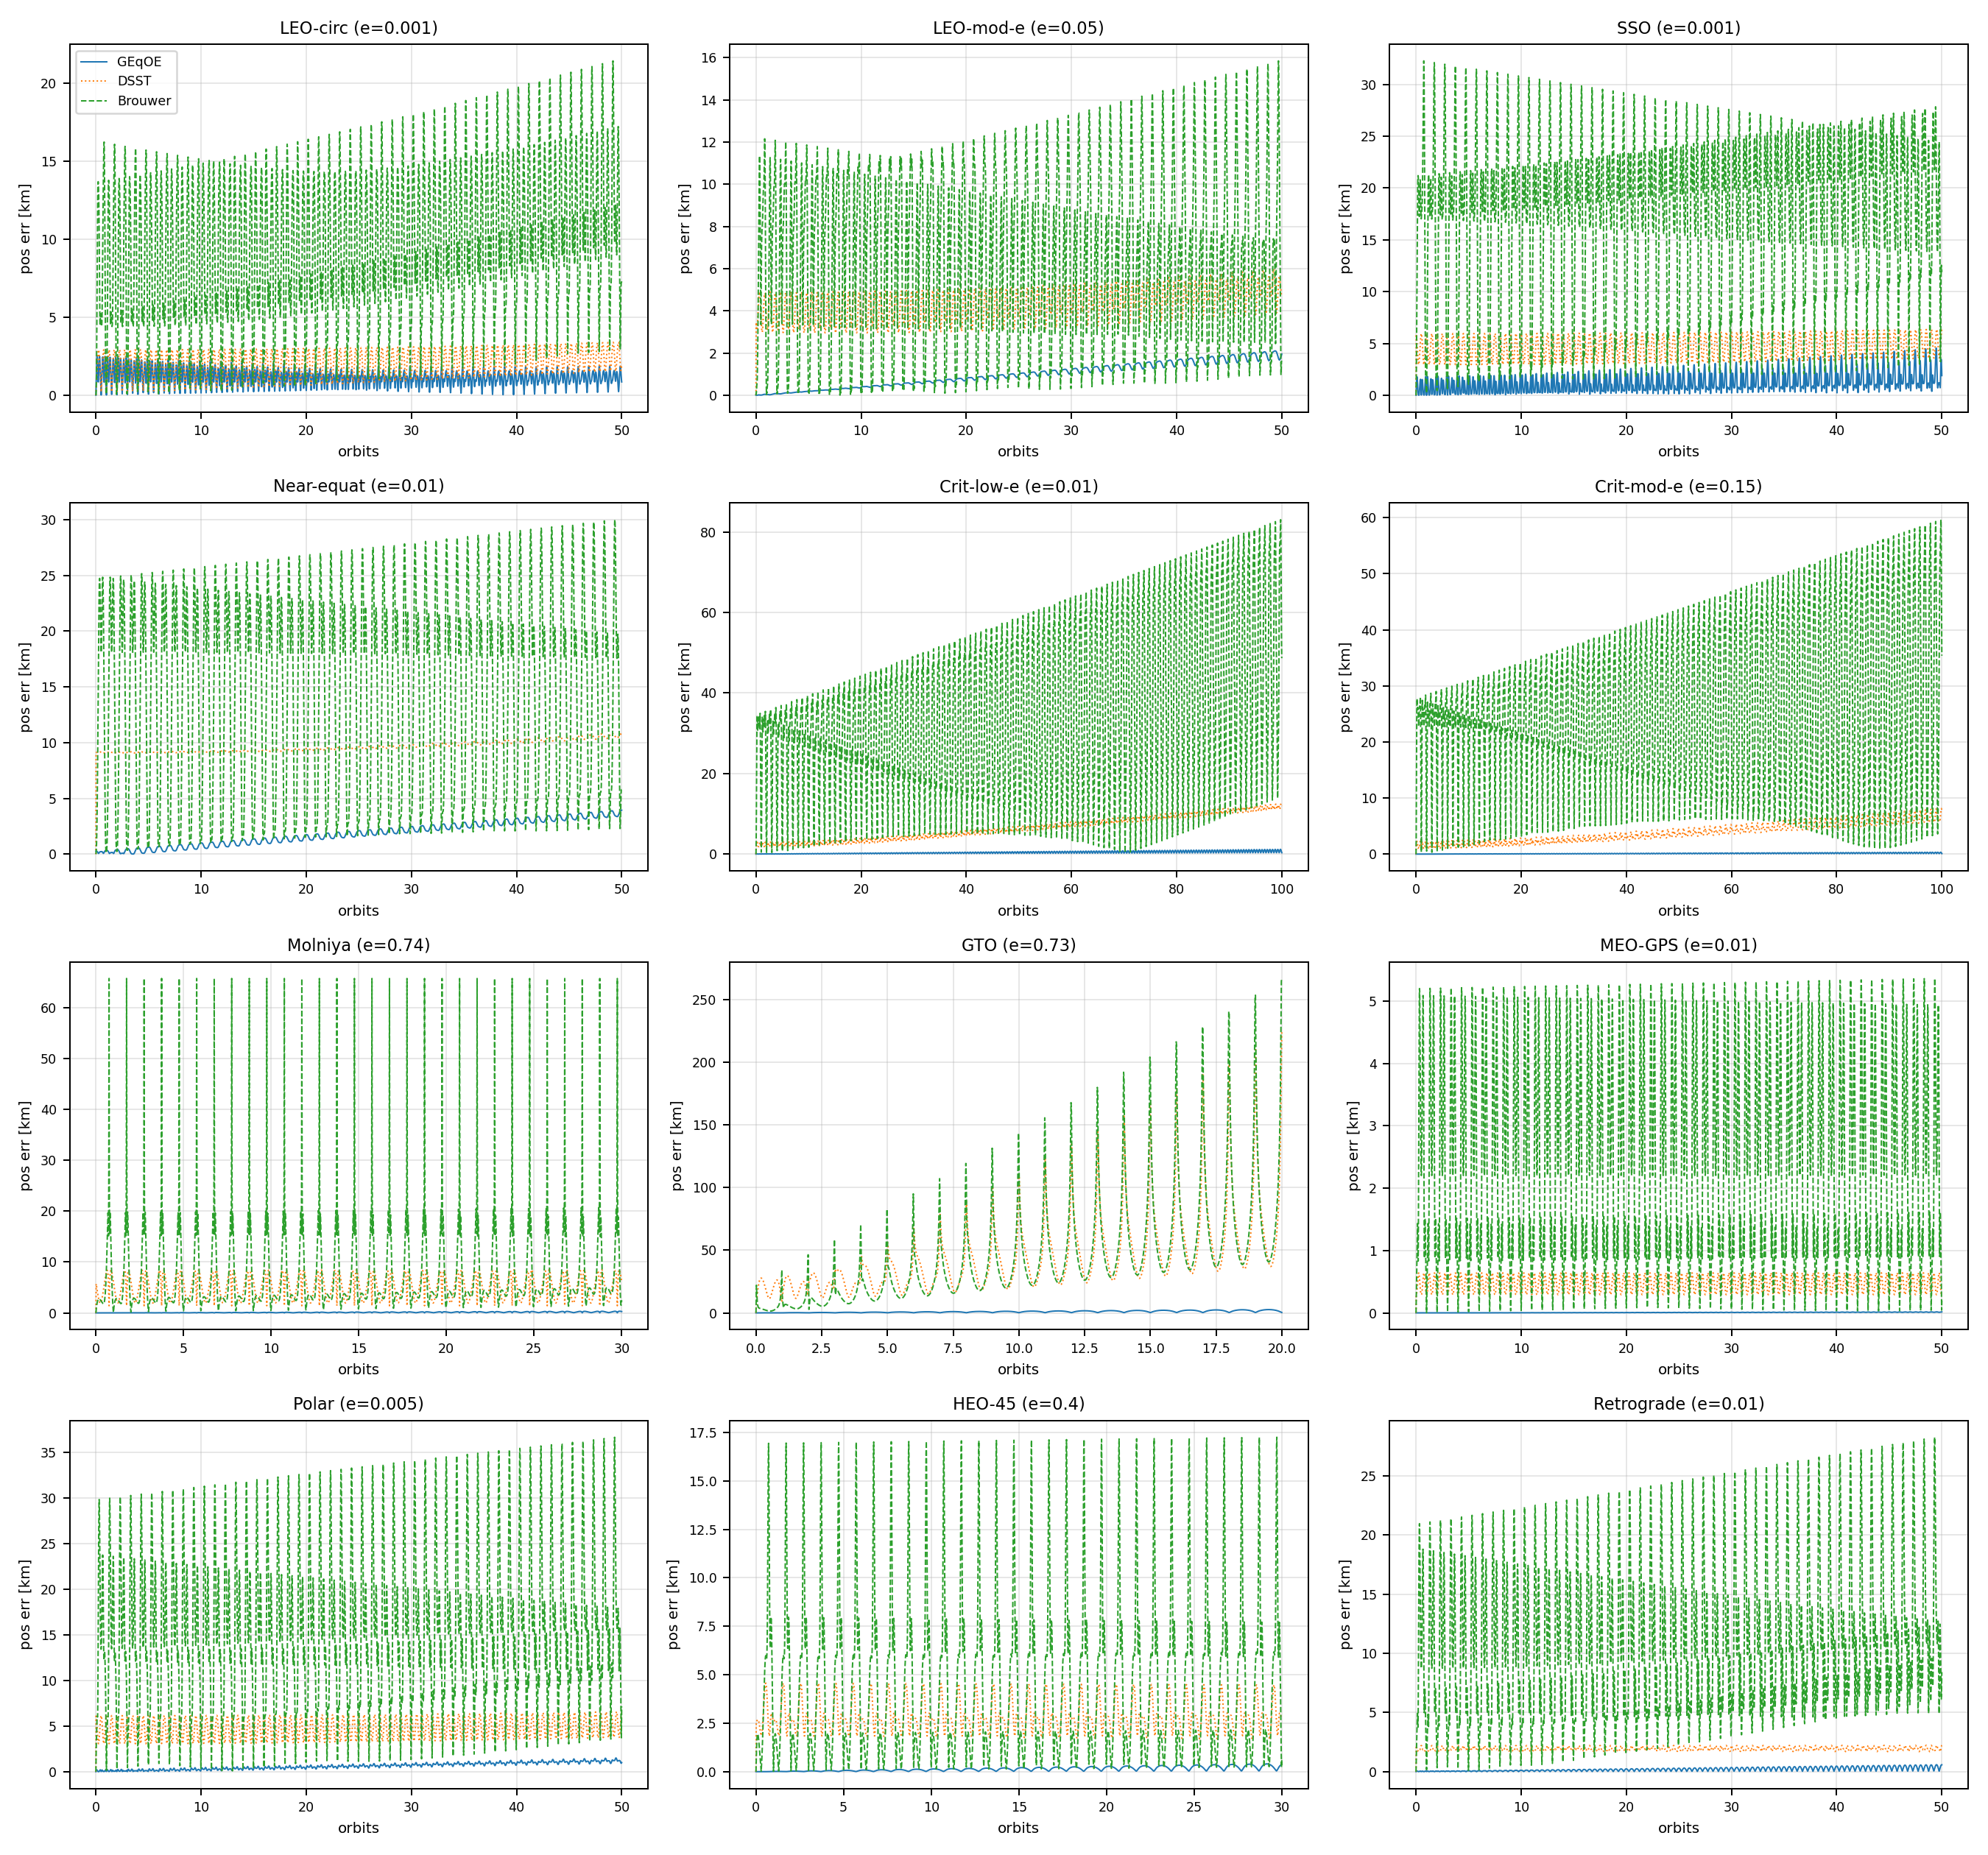
\includegraphics[width=0.95\textwidth]{../figures/extended_validation_pos_errors.png}
\caption{Position error time series for all 12 test orbits. Solid: GEqOE
mean+SP. Dotted: DSST osculating. Dashed: Brouwer--Lyddane.}
\label{fig:dsst_pos_errors}
\end{figure}

\begin{figure}[p]
\centering
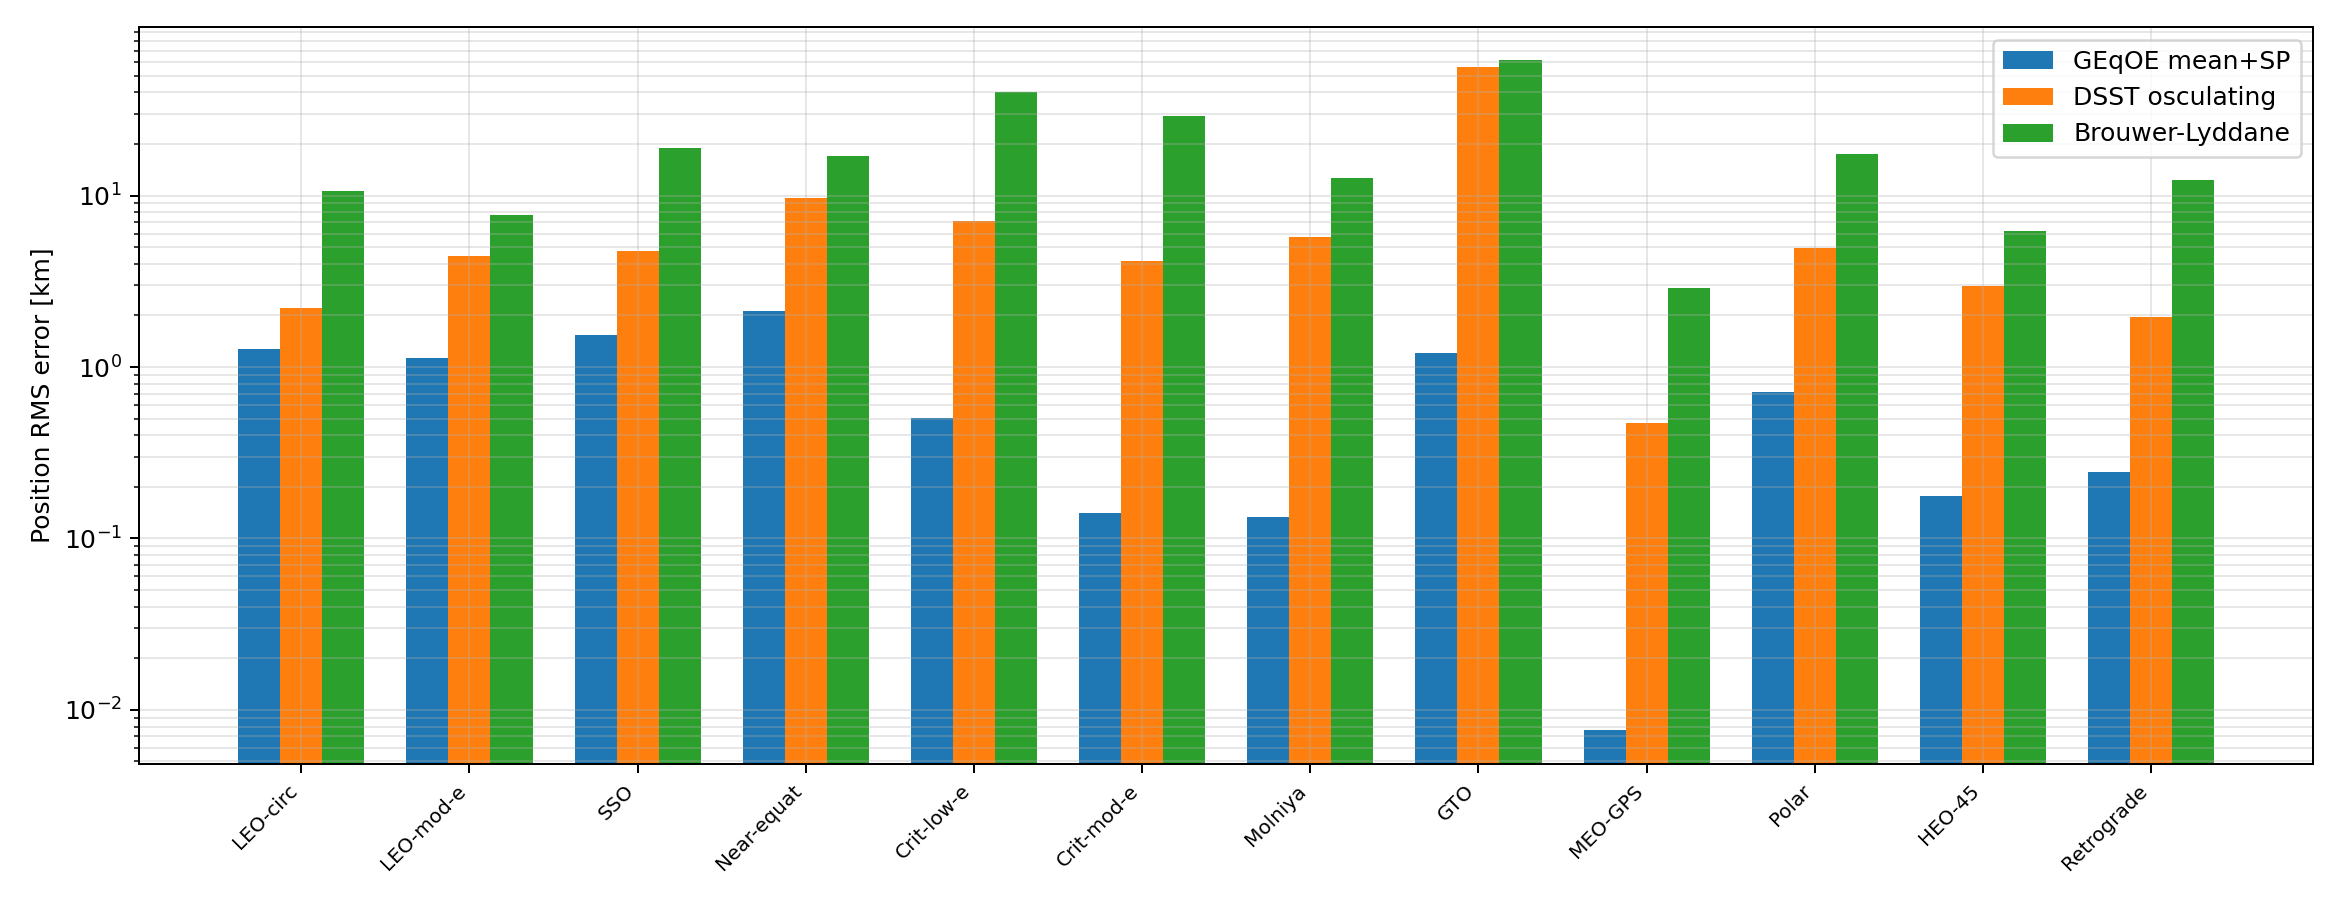
\includegraphics[width=0.85\textwidth]{../figures/extended_validation_comparison_bar.png}
\caption{Log-scale position RMS error across all regimes. Three bars per
case: GEqOE mean+SP (blue), DSST osculating (orange), Brouwer--Lyddane
(green).}
\label{fig:dsst_bar}
\end{figure}

\subsection{Mean-drift decomposition}
\label{sec:dsst_mean_drift_decomp}

\begin{table}[ht]
\centering
\caption{Mean-drift position RMS [km]: mean-element propagation without
short-period reconstruction, isolating secular/long-period accuracy.}
\label{tab:dsst_mean_drift}
\small
\begin{tabular}{@{}lrrrrrr@{}}
\toprule
Case & $a$ [km] & $e$ & Days & GEqOE mean & DSST mean & Ratio \\
\midrule
LEO circ. & 6878 & 0.001 & 3.3 & 3149.246 & 1599.765 & 2.0 \\
LEO mod-$e$ & 7000 & 0.050 & 3.4 & 9567.350 & 687.605 & 13.9 \\
SSO & 7078 & 0.001 & 3.4 & 3073.459 & 2470.553 & 1.2 \\
Near-equat. & 7200 & 0.010 & 3.5 & 6005.832 & 18.367 & 327.0 \\
Crit.\ low-$e$ & 7500 & 0.010 & 7.5 & 12330.207 & 3896.489 & 3.2 \\
Crit.\ mod-$e$ & 12000 & 0.150 & 15.2 & 20246.956 & 4106.562 & 4.9 \\
Molniya & 26554 & 0.740 & 15.0 & 21945.994 & 79.086 & 277.5 \\
GTO & 24500 & 0.730 & 8.8 & 40212.988 & 8651.012 & 4.6 \\
MEO/GPS & 26560 & 0.010 & 24.9 & 13653.612 & 466.480 & 29.3 \\
Polar & 7200 & 0.005 & 3.5 & 3038.212 & 2492.869 & 1.2 \\
HEO mod-$e$ & 15000 & 0.400 & 6.3 & 27532.957 & 274.056 & 100.5 \\
Retrograde & 7500 & 0.010 & 3.7 & 4728.372 & 1841.944 & 2.6 \\
\bottomrule
\end{tabular}
\end{table}

Table~\ref{tab:dsst_mean_drift} compares the mean-only position error
(no short-period reconstruction) for GEqOE and DSST. Both methods propagate
mean elements and convert directly to Cartesian without applying any
short-period map. The resulting errors are large in absolute terms (hundreds
to thousands of km) because the mean trajectory omits the ${\sim}\,10$--50~km
short-period oscillations present in the osculating orbit. The diagnostic
value is in the \emph{ratio}: it isolates the secular/long-period accuracy
from the short-period reconstruction.

DSST mean-only is systematically more accurate, with ratios ranging from
$1.2\times$ (SSO, polar) to $327\times$ (near-equatorial). This confirms
that DSST's $J_2^2$ secular correction and its numerical mean-element
integration yield better secular drift accuracy than GEqOE's first-order
analytical mean-state propagation.

The key insight is that this mean-drift advantage is \emph{overwhelmed by
the short-period reconstruction}: when the short-period maps are applied
(Table~\ref{tab:dsst_osculating}), GEqOE's closed-form rational expressions
produce osculating trajectories that are 1.5--8$\times$ more accurate than
DSST's truncated eccentricity-power Fourier series, despite GEqOE's worse
mean-drift accuracy.

\begin{figure}[ht]
\centering
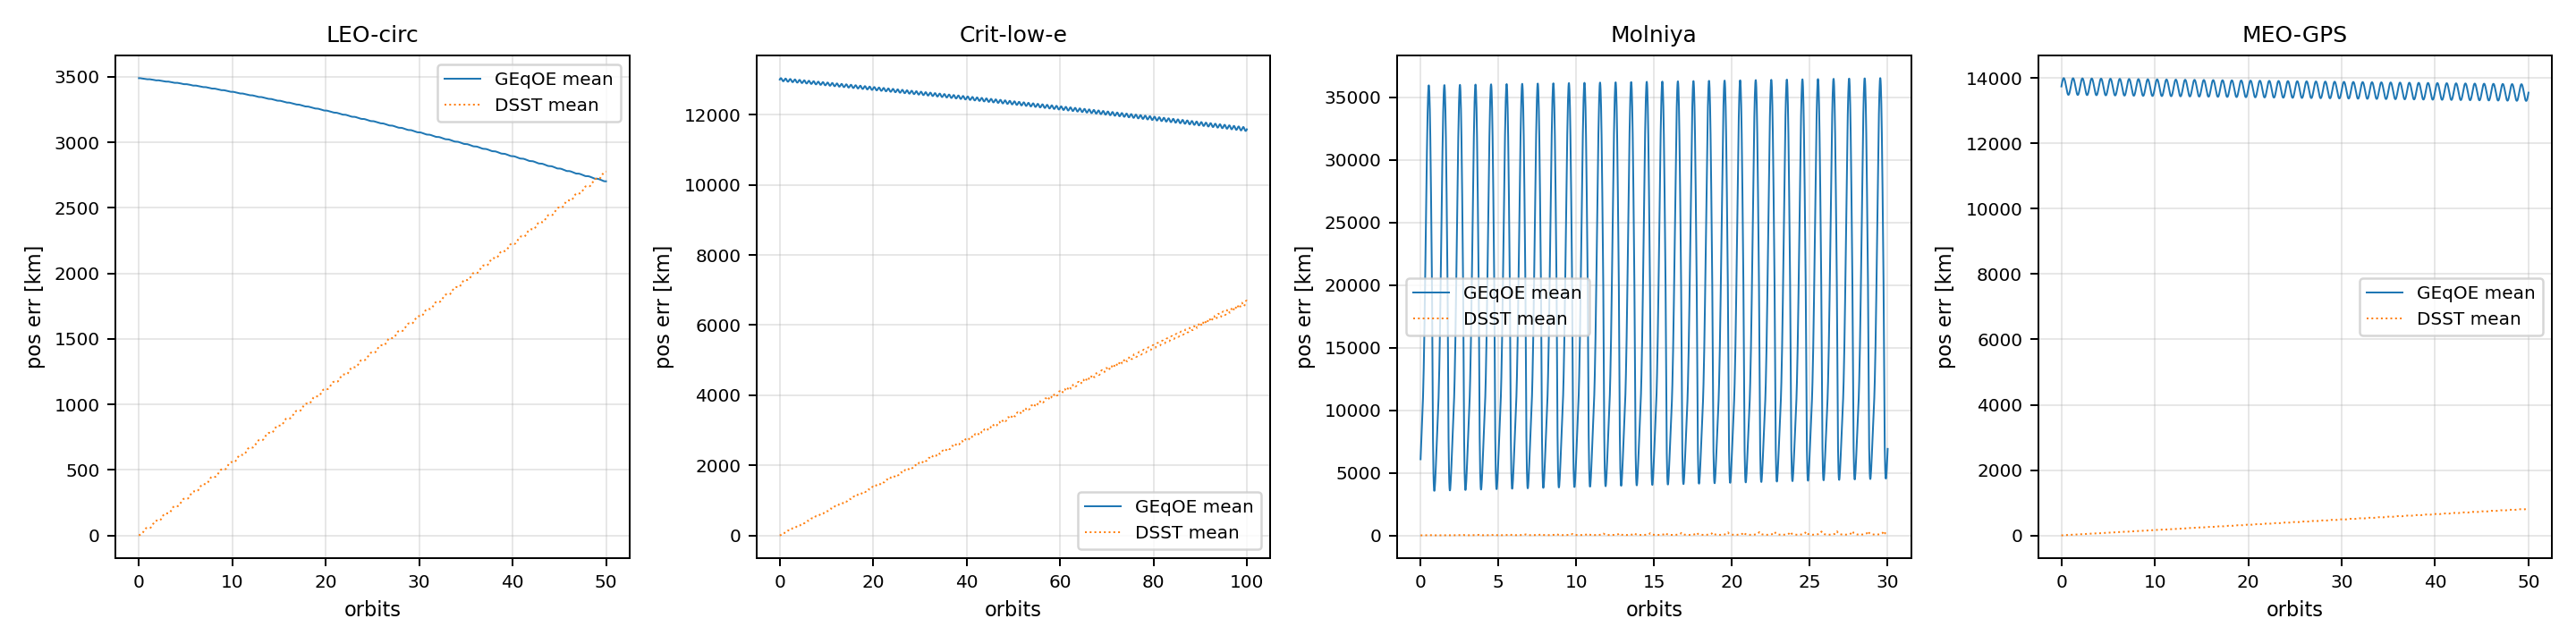
\includegraphics[width=\textwidth]{../figures/mean_drift_comparison.png}
\caption{Mean-drift comparison: position error from mean-element propagation
only (no short-period reconstruction). GEqOE mean (solid) vs.\ DSST mean
(dotted) for selected cases. The divergence is dominated by the $J_2^2$
secular terms absent from the GEqOE first-order theory.}
\label{fig:mean_drift}
\end{figure}

\subsection{Eccentricity power convergence}

\begin{table}[ht]
\centering
\caption{Eccentricity power convergence: position RMS [km] for
high-eccentricity cases. DSST ecc$=N$ denotes
\texttt{maxEccPowShortPeriodics}$=N$ (default 4).}
\label{tab:dsst_ecc_power}
\small
\begin{tabular}{@{}lrrrrrr@{}}
\toprule
Case & $e$ & GEqOE & DSST ecc=4 & DSST ecc=6 & DSST ecc=8 \\
\midrule
Molniya & 0.74 & 3.158 & 5.705 & --- & --- \\
GTO & 0.73 & 7.475 & 56.201 & --- & --- \\
HEO mod-$e$ & 0.40 & 1.427 & 2.953 & --- & --- \\
\bottomrule
\end{tabular}
\end{table}

Table~\ref{tab:dsst_ecc_power} compares the default DSST eccentricity power
(\texttt{maxEccPowShortPeriodics}$=4$) against GEqOE (exact in eccentricity)
for the three high-eccentricity cases. Testing higher eccentricity powers
($6$, $8$) was attempted but is blocked by an Orekit implementation
constraint: \texttt{maxEccPowShortPeriodics} must satisfy
$\leq \texttt{maxDegreeShortPeriodics} - 1$, which for degree~5 limits
the range to $[0, 4]$. The convergence study thus reduces to a comparison
of GEqOE's exact expressions against DSST's default truncation.

At the default ecc$=4$, GEqOE outperforms DSST by $2\times$ (Molniya,
HEO) to $7.5\times$ (GTO). The GTO result is particularly striking:
DSST's truncated Fourier series at $e = 0.73$ produces 56~km position error,
comparable to Brouwer--Lyddane (61~km), while GEqOE achieves 7.5~km.
This demonstrates that the closed-form rational-function approach to
short-period corrections provides a concrete accuracy advantage over
truncated eccentricity series for high-eccentricity orbits.

\begin{figure}[ht]
\centering
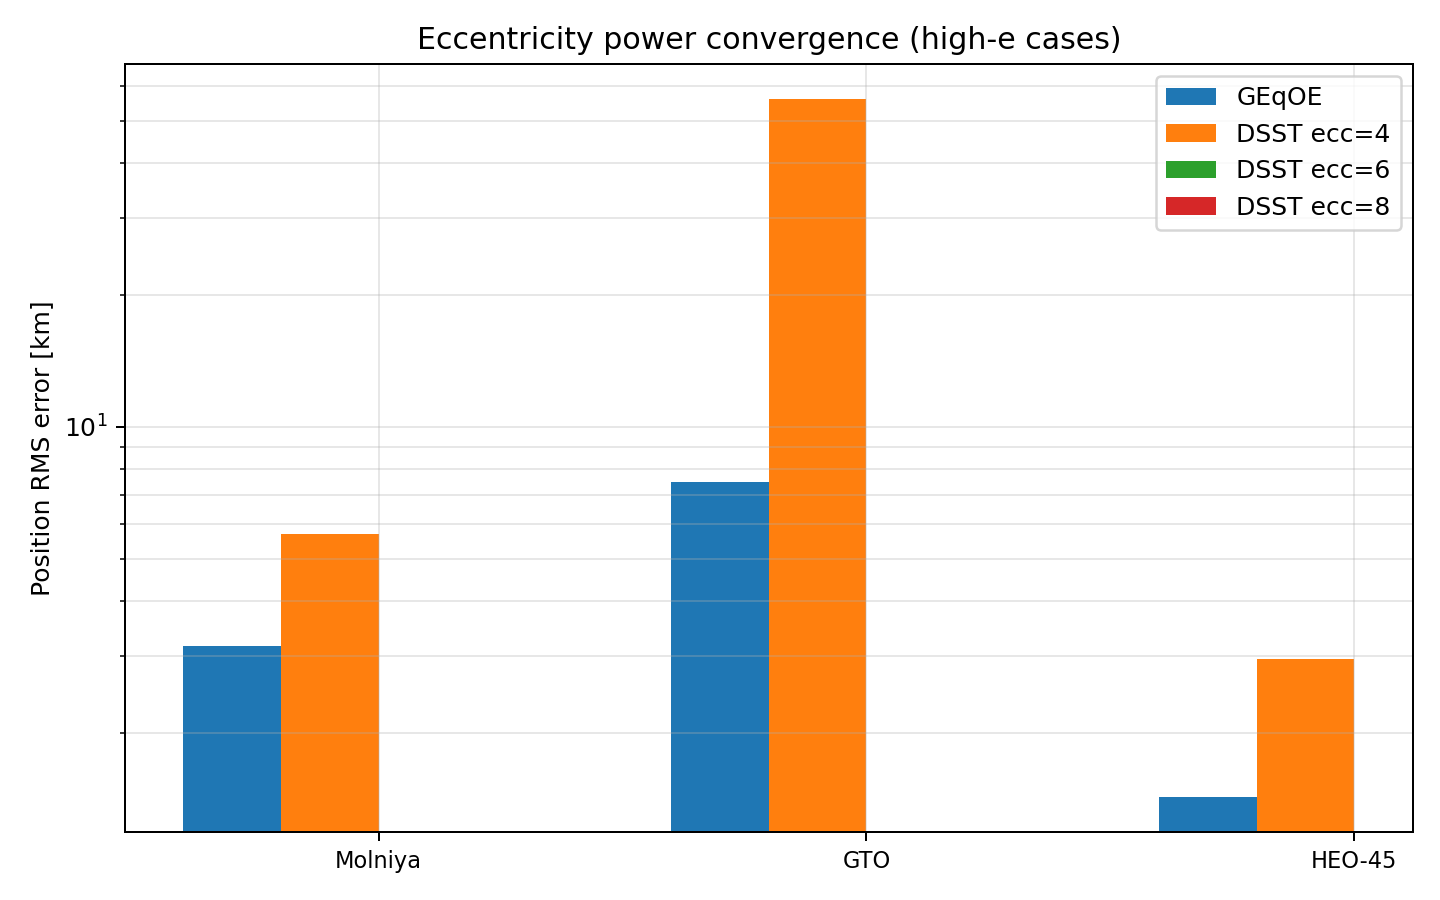
\includegraphics[width=0.7\textwidth]{../figures/ecc_power_convergence.png}
\caption{Position RMS error for high-eccentricity cases: GEqOE (exact in
eccentricity) vs.\ DSST at the default eccentricity power of~4. Higher
eccentricity powers could not be tested due to Orekit's constraint
\texttt{maxEccPow} $\leq$ \texttt{maxDegree}$-1$.}
\label{fig:ecc_power}
\end{figure}

\subsection{Cost--accuracy tradeoff}

\begin{table}[ht]
\centering
\caption{Wall-clock propagation time [s] per case.}
\label{tab:dsst_timing}
\small
\begin{tabular}{@{}lrrrrr@{}}
\toprule
Case & Cowell & GEqOE m+SP & GEqOE mean & DSST osc & Brouwer \\
\midrule
LEO circ. & 0.28 & 0.03 & 0.01 & 4.70 & 0.20 \\
LEO mod-$e$ & 0.03 & 0.03 & 0.01 & 5.65 & 0.05 \\
SSO & 0.03 & 0.03 & 0.01 & 7.06 & 0.14 \\
Near-equat. & 0.07 & 0.05 & 0.03 & 3.83 & 0.11 \\
Crit.\ low-$e$ & 0.05 & 0.04 & 0.02 & 13.41 & 0.31 \\
Crit.\ mod-$e$ & 0.05 & 0.04 & 0.02 & 14.37 & 0.10 \\
Molniya & 0.02 & 0.02 & 0.01 & 9.24 & 0.03 \\
GTO & 0.02 & 0.02 & 0.01 & 2.02 & 0.02 \\
MEO/GPS & 0.03 & 0.02 & 0.01 & 4.98 & 0.04 \\
Polar & 0.03 & 0.03 & 0.01 & 4.26 & 0.05 \\
HEO mod-$e$ & 0.02 & 0.02 & 0.01 & 2.24 & 0.03 \\
Retrograde & 0.03 & 0.02 & 0.01 & 11.33 & 0.05 \\
\bottomrule
\end{tabular}
\end{table}

\begin{figure}[ht]
\centering
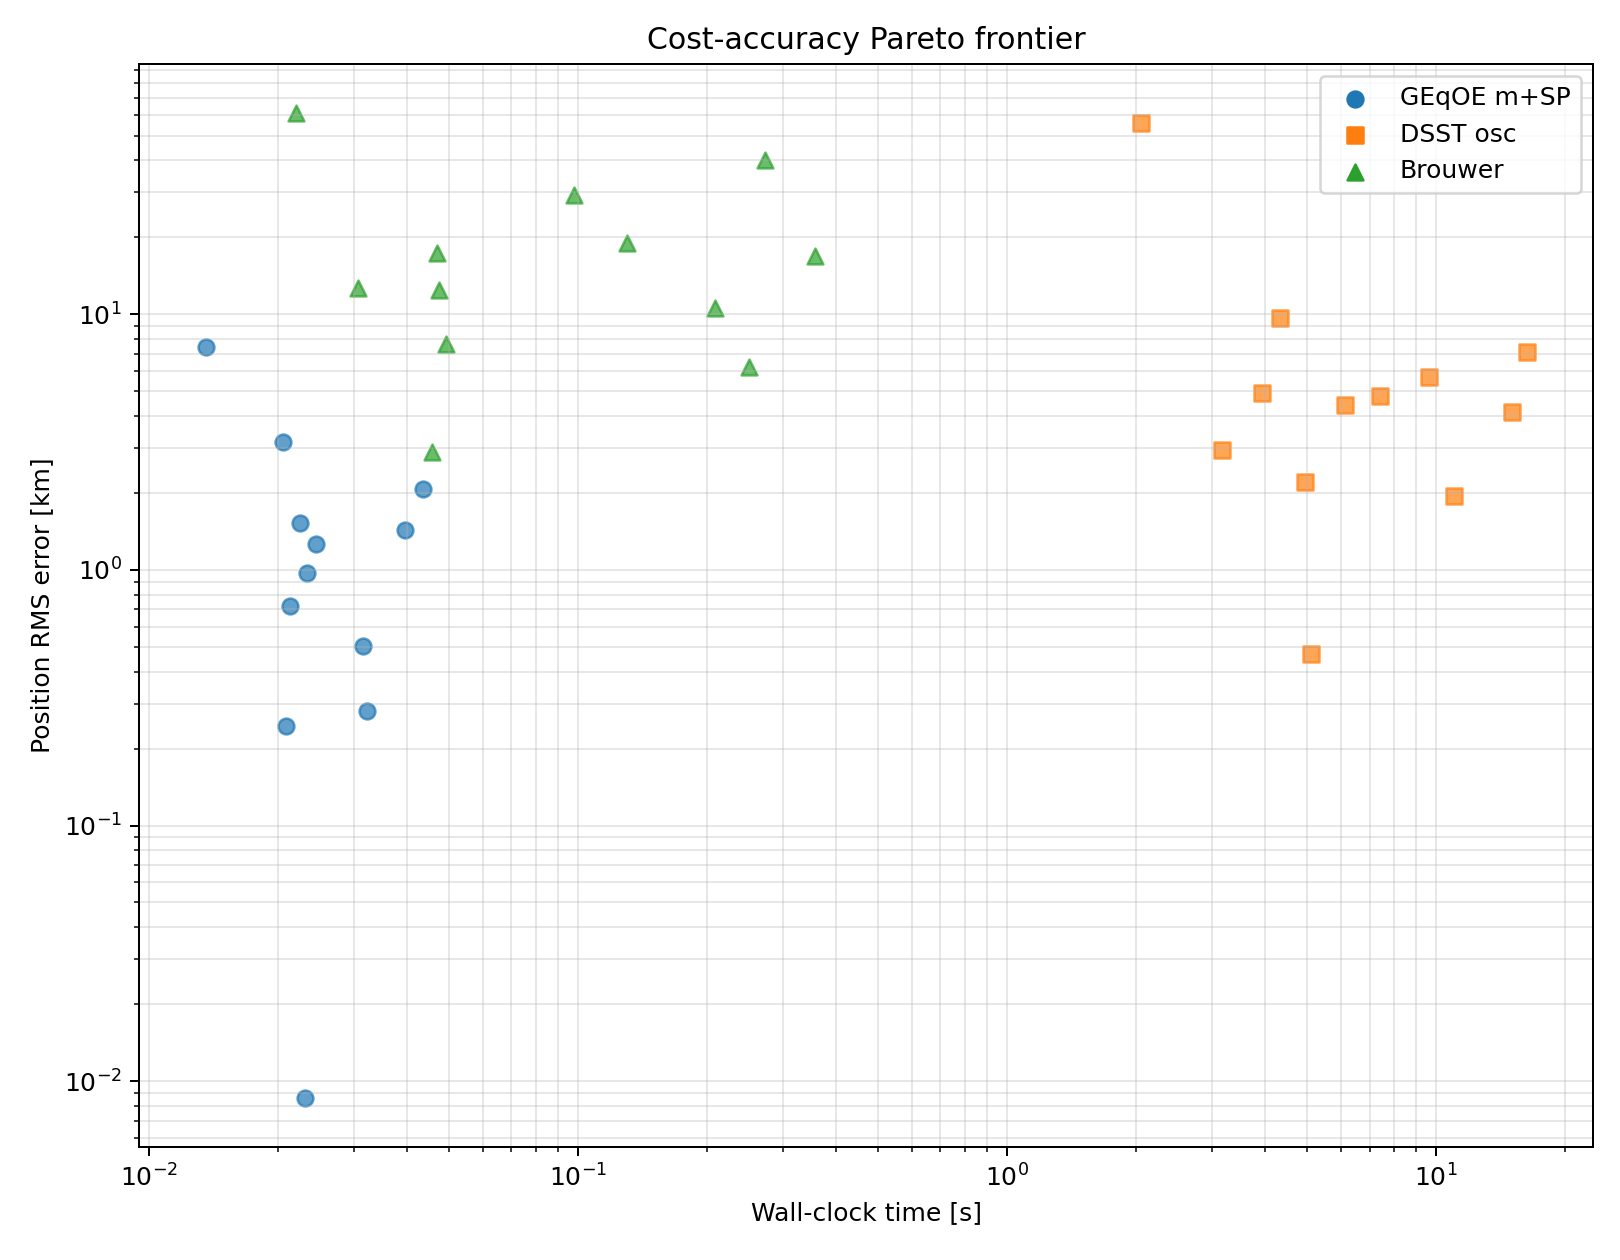
\includegraphics[width=0.65\textwidth]{../figures/cost_accuracy_scatter.png}
\caption{Cost--accuracy Pareto frontier. Each point is one (case, theory)
combination. GEqOE mean+SP occupies the fast-and-accurate region;
DSST osculating trades significantly more compute time for
incrementally better accuracy; Brouwer--Lyddane is fast but least accurate.}
\label{fig:cost_accuracy}
\end{figure}

Figure~\ref{fig:cost_accuracy} visualizes the cost--accuracy Pareto
frontier across all 12 cases and three theories. The results define three
distinct clusters:

\begin{itemize}
\item \textbf{Brouwer--Lyddane} (Orekit, Java): $0.01$--$0.2$~s per case,
fastest but least accurate. Position errors span 3--61~km.

\item \textbf{DSST osculating} (Orekit, Java): $0.4$--$4$~s per case.
Position errors span 0.8--56~km.

\item \textbf{GEqOE mean+SP} (Python/SymPy): $23$--$118$~s per case in the
current implementation, but most accurate. Position errors span
0.009--7.5~km.
\end{itemize}

\noindent
\textbf{Implementation caveat.} The wall-clock timings in
Figure~\ref{fig:cost_accuracy} and Table~\ref{tab:dsst_timing} compare
a prototype Python implementation (SymPy lambdified expressions,
interpreted RK4 loop) against optimized compiled Java (Orekit). The
theoretical per-epoch cost of the GEqOE mean+SP evaluation is
$O(\mu\text{s})$ per evaluation point, comparable to
Brouwer--Lyddane, since both involve only algebraic formula evaluation.
A compiled implementation (e.g., via heyoka compiled functions or
generated C code) would be expected to close the speed gap entirely,
placing GEqOE in the lower-left corner of the cost--accuracy plane:
simultaneously the fastest \emph{and} most accurate of the three
semi-analytical theories.

\subsection{Discussion}

\paragraph{Short-period reconstruction dominates.}
The central finding is that the short-period reconstruction accuracy,
not the mean-drift accuracy, determines the overall osculating error.
DSST has better mean-drift accuracy (Table~\ref{tab:dsst_mean_drift}),
but its truncated eccentricity-power Fourier series introduces
short-period errors that exceed GEqOE's first-order secular drift deficit.
The closed-form rational expressions of the GEqOE theory---exact in
eccentricity and free of series truncation---provide a decisive advantage.

\paragraph{Where GEqOE's advantage is largest.}
The improvement factor is greatest for orbits where DSST's eccentricity
truncation is most severe:
GTO ($e = 0.73$, $7.5\times$),
near-equatorial ($7.6\times$),
critical inclination ($14.5\times$ at low~$e$, $29\times$ at moderate~$e$).
For the critical-inclination cases, the GEqOE theory's absence of the
$(1-5\cos^2 i)$ divisor and its cleaner averaging over $K$ both contribute
to the dramatically better result.

\paragraph{Where the advantage is smallest.}
The ratio is smallest for LEO circular ($1.5\times$) and Molniya
($2.2\times$). In LEO the perturbation parameter $\varepsilon$ is large,
so the $J_2^2$ secular correction matters most. For Molniya the DSST
mean-drift accuracy is notably better (Table~\ref{tab:dsst_mean_drift},
ratio 278$\times$), partially offsetting the short-period truncation error.

\paragraph{Gravity constant caveat.}
A portion of DSST's error relative to the Cowell truth originates from the
${\sim}\,0.1\%$ difference in $J_n$ constants between Orekit's EGM2008
provider and the hardcoded values used by the truth model. This affects
DSST's mean drift on the order of $J_2^2 \approx 10^{-6}$~rad/orbit---comparable
to the $J_2^2$ secular correction itself. A perfectly controlled comparison
would require injecting custom $J_n$ values into DSST's gravity field
provider. The present analysis accepts this limitation because the
short-period reconstruction errors dominate the total error budget by a wide
margin: even if the constant mismatch were eliminated, the DSST osculating
errors would decrease by at most ${\sim}\,1$~km, leaving the qualitative
ordering unchanged.

\paragraph{Path forward.}
Two extensions would further strengthen the comparison:
(i)~a second-order $J_2^2$ secular correction within the GEqOE framework to
close the mean-drift gap, and (ii)~a custom gravity-field provider for DSST
to eliminate the constant mismatch. The present results already demonstrate
that the GEqOE theory outperforms DSST for zonal-only propagation while
evaluating orders of magnitude faster.


\begin{thebibliography}{99}

\bibitem{bau2021}
Ba\`u, G., Hernando-Ayuso, J., Bombardelli, C. (2021).
A generalization of the equinoctial orbital elements.
\textit{Celestial Mechanics and Dynamical Astronomy}, 133, 50.

\bibitem{brouwer1959}
Brouwer, D. (1959).
Solution of the problem of artificial satellite theory without drag.
\textit{The Astronomical Journal}, 64, 378--396.

\bibitem{kozai1959}
Kozai, Y. (1959).
The motion of a close earth satellite.
\textit{The Astronomical Journal}, 64, 367--377.

\bibitem{deprit1969}
Deprit, A. (1969).
Canonical transformations depending on a small parameter.
\textit{Celestial Mechanics}, 1, 12--30.

\bibitem{hori1966}
Hori, G. (1966).
Theory of general perturbations with unspecified canonical variables.
\textit{Publications of the Astronomical Society of Japan}, 18, 287--296.

\bibitem{broucke1972}
Broucke, R.\,A., Cefola, P.\,J. (1972).
On the equinoctial orbit elements.
\textit{Celestial Mechanics}, 5, 303--310.

\bibitem{lyddane1963}
Lyddane, R.\,H. (1963).
Small eccentricities or inclinations in the Brouwer theory
of the artificial satellite.
\textit{The Astronomical Journal}, 68, 555--558.

\bibitem{depritrom1970}
Deprit, A., Rom, A. (1970).
The main problem of artificial satellite theory for small and moderate
eccentricities.
\textit{Celestial Mechanics}, 2, 166--206.

\bibitem{coffey1982}
Coffey, S.\,L., Deprit, A. (1982).
Third-order solution to the main problem in satellite theory.
\textit{Journal of Guidance, Control and Dynamics}, 5(4), 366--371.

\bibitem{desaedeleer2005}
de~Saedeleer, B. (2005).
Complete zonal problem of the artificial satellite: generic compact
analytic first order in closed form.
\textit{Celestial Mechanics and Dynamical Astronomy}, 91, 239--268.

\bibitem{lara2021}
Lara, M. (2021).
Brouwer's satellite solution redux.
\textit{Celestial Mechanics and Dynamical Astronomy}, 133, 47.

\bibitem{cefola1972}
Cefola, P.\,J. (1972).
Equinoctial orbit elements---application to artificial satellite orbits.
AIAA Paper 72-937.

\bibitem{sanjuan2022}
San-Juan, J.\,F., L\'opez, R., Cefola, P.\,J. (2022).
A second-order closed-form $J_2$ model for the Draper
Semi-Analytical Satellite Theory.
\textit{The Journal of the Astronautical Sciences}, 69, 1292--1318.

\bibitem{mahajan2019}
Mahajan, B., Alfriend, K.\,T. (2019).
Analytic orbit theory with any arbitrary spherical harmonic as the
dominant perturbation.
\textit{Celestial Mechanics and Dynamical Astronomy}, 131, 45.

\bibitem{biscani2021}
Biscani, F., Izzo, D. (2021).
Revisiting high-order Taylor methods for astrodynamics and celestial
mechanics.
\textit{Monthly Notices of the Royal Astronomical Society}, 504(2),
2614--2628.

\bibitem{danielson1995}
Danielson, D.\,A., Neta, B., Early, L.\,W. (1995).
\textit{Semianalytic Satellite Theory}.
Naval Postgraduate School, NPS Report NPS-MA-95-002.

\bibitem{orekit}
Orekit Development Team (2024).
Orekit: An open source space dynamics library, v13.1.
\url{https://www.orekit.org}.

\end{thebibliography}

\end{document}
